\documentclass[a4paper]{article}

%% Language and font encodings
\usepackage[english]{babel}
\usepackage[utf8x]{inputenc}
\usepackage[T1]{fontenc}


%% Sets page size and margins
\usepackage[a4paper,top=3cm,bottom=2cm,left=3cm,right=3cm,marginparwidth=1.75cm]{geometry}

%% Useful packages
\usepackage{amsmath}
\usepackage{graphicx}
\usepackage{tikz,pgfplots}
\usepackage[colorinlistoftodos]{todonotes}
\usepackage[colorlinks=true, allcolors=blue]{hyperref}
\usepackage{amsfonts}
\usepackage{bbm}
\usepackage{dsfont}
\usepackage{cancel}
\usepackage{tikz,tkz-base,tkz-fct}
\usepackage{pgfplots}
\newcommand{\prob}{\mathbb{P}}
\newtheorem{definicion}{Definición}
\newtheorem{teorema}{Teorema}
\newtheorem{ejemplo}{Ejemplo}
\DeclareMathOperator*{\argmax}{Arg\,max}
\newtheorem{lem}{Lema}
\newtheorem{prop}{Proposici\'on}
\newtheorem{cor}{Corolario}
\newtheorem{dem}{Demostración}
\numberwithin{equation}{subsection}
\newtheorem{obs}{Observación}


%% Aquí se pueden definir nuevas abreviaturas para algunos comandos

\def\sen{{\rm sen\mspace{1.5mu}}}
\def\C{\mathbb C}
\def\R{\mathbb R}
\def\N{\mathbb N}
\def\Q{\mathbb Q}
\def\Z{\mathbb Z}
\def\V{\mathbb V}
\def\E{\mathbb E}
\def\to{\rightarrow}
\newcommand{\pb}{\mathbb{P}}



\newcommand{\ds}{\displaystyle}


%Para hacer normas en tex

\providecommand{\norm}[1]{\lVert#1\rVert}
\providecommand{\normm}[1]{\bigg\lVert#1\bigg\rVert}


%integrales bacanes
\usepackage{ esint }

%Para poner en negrita en modo matemático
\newcommand{\negri}{\boldsymbol}




\title{Simulación Estocástica}
\author{Apuntes de clase.}
\date{2019}

\begin{document}
\maketitle
\tableofcontents
\newpage
\section{Notación}
\begin{itemize}
    \item $i.i.d.$: 'Independientes e idénticamente distribuídas'.
    \item $(E,d)$: Espacio métrico $E$, con métrica $d$.
    \item $\mathcal{B}(E)$: Conjunto de borelianos de $E$.
    \item $C_b (E) := \{f:E \rightarrow R \,| \text{ f es contínua y acotada}\}$
    \item $\mathcal{P}(E)$: Espacio de las medidas de probabilidades sobre $E$.
    \item $c.s.$: "Casi seguramente"
    \item \textbf{T.C.D.}: "Teorema de convergencia  dominada".
    \item $\mathcal{N}(\mu,\sigma)$: "Distribución normal de media $\mu$ y desviación estándar de $\sigma$", se hará un abuso de notación ya que también simbolizará la variable aleatoria que distribuya de esta forma.
    \item $M.M.C.$: "Método de Monte Carlo".
    \item $C.M.H.$: "Cadena de Markov homogénea".
    \item $M.C.M.C.$: "Markov chain Monte Carlo".
\end{itemize}

\section{Convergencia en Ley}
Partiremos este capítulo enunciando uno de los teoremas más importante de la teoría de probabilidades, el teorema del límite central.

\begin{teorema}[Teorema Central del Límite.] Dadas $(X_n)_{n\in\N}$ variables aleatorias $i.i.d.$, con \newline$\mu = \E(X_1)$ y $\sigma^2 = Var(X_1)$, finitas. Para el promedio $n-esimo$:
\begin{equation}
    \Bar{X}_n = \frac{1}{n}\sum_{i=1}^{n}X_i
\end{equation}
Se define la variable aleatoria $Z_n$ como:
\begin{equation}
    Z_n = \frac{\Bar{X}_n - \mu}{\sigma / \sqrt{n}}
\end{equation}
Entonces $Z_n$ converge "EN LEY" a una variable normal estándar $\mathcal{N}(0,1)$ a medida que $n$ tiende a infinito.
\end{teorema}

Los resultados y usos que se desprenden de este teorema son bastante variados; desde el cálculo de probabilidades para una muestra aleatoria simple, estimación de parámetros, hasta nos premite el uso de test de hipótesis para distribuciones normales en ocaciones en que desconocemos por completo la distribución de los datos.\footnote{Todos estos usos están restringidos bajo aproximaciones.}\\ \newline
Y no es que sea raro encontrar este tipo de usos, puesto que el teorema no nos pide absolutamente nada con respecto al tipo de  distribución de las variables aleatorias, dando la posibilidad de que éstas sean contínuas, discretas o cualesquiera que se nos pudiesen ocurrir en diversos espacios de trabajo. Sin embargo el resultado es el mimso, convergencia a una distribución absolutamente contínua.\\ \newline
Si $Z_n$ puede tomar varias formas dada la colección de variables $(X_n)_{n\in\N}$, ¿por qué converge a una distribución contínua? Para responder esta pregunta introduciremos las nociones de \textit{convergencia débil de medida de probabilidad}.\newpage

\subsection{Convergencia débil sobre espacios métricos}

Para el conjunto de medidas de probabilidad sobre el espacio métrico $E$, es decir; $\mathcal{P}(E)$, definiremos la siguiente operación.\\ Para toda $\mu \in \mathcal{P}(E)$ y para toda $f: E\rightarrow \R$ función medible:
\begin{equation}
    \langle \mu , f\rangle = \int_{E} f d\mu
\end{equation}
\begin{definicion} Decimos que una sucesión $(\mu_n)_{n\in\N}$ de elementos de $\mathcal{P}(E)$ converge DEBILMENTE a $\mu\in \mathcal{P}(E)$ si:
\[\langle \mu_n ,f\rangle\, \xrightarrow{n\rightarrow\infty}\, \langle \mu,f\rangle \hspace{0.5cm}\forall\,f\in C_b(E)\]
En tal caso anotamos: $\mu_n \Rightarrow \mu$.
\end{definicion}

\begin{ejemplo}
    Tomemos el espacio métrico $E=\R$ con su métrica usual $d(x,y) = |x-y|$, y sea la sucesión de medidas de probabilidad $\mu_n = \delta_{\frac{1}{n}}$, donde $\delta_a$ representa la "Delta de Dirac" en el punto $a$:
    \[\delta_a(x) = \begin{cases} 
            +\infty & \text{si }x=a   \\ 
            0 & \text{si }x\neq a \end{cases}\]
    
    Veremos que esta distribución converge débilmente a la distribución $\delta_0$.\\ \newline
    En efecto, sea $f \in C_b(\R)$, tenemos que:
    \[\langle \mu_n ,f\rangle = \int_\R f(x) \mu_n (dx) = \int_\R f(x) \delta_{\frac{1}{n}}(x) dx = f(1/n)\]
    Puesto que la función $f$ es contínua en todo $\R$, entonces:
    \[f(1/n) \xrightarrow{n\rightarrow\infty}\,f(0) = \langle \mu,f\rangle \]
    Por lo tanto, $\mu_n \Rightarrow \mu$.
\end{ejemplo}
Dado que el argumento utilizado en el ejemplo se sostuvo fuertemente de la continuidad de la función $f$, en general se tendrá que para cada sucesión de reales $(x_n)_n$ que converja a un punto $\Bar{x}$, se tendrá la convergencia de las medidas de Dirac: $\delta_{x_n}\Rightarrow \delta_{\Bar{x}}$. Se puede demostrar que esto es una doble implicancia, es decir; la convergencia debil de las medidas de Dicar implican la convergencia en $\R$ de la sucesión de los puntos.\\ \newline
Para traducir el \textit{teorema Central del Límite} en conceptos de convergencia de medidas de probabilidad debemos asociar el concepto de \textit{variable aleatoria} en función de la medida de probabilidad asociada.\\
Recordemos que una variable aleatoria a valores en $E$ es una función $X:\Omega \rightarrow E$ medible, donde $(\Omega, \mathcal{F},\pb)$ es un espacio de probabilidad (este espacio se encuentra usualmente implícito en la mayoría de las definiciones y cálculos de probabilidades).\\ Su LEY o DISTRIBUCIÓN, denotada como $\mathcal{L}(X) \in \mathcal{P}(E)$, se definie como:
\begin{equation}
   \mathcal{L}(X)(A) := \pb(X^{-1}(A))\hspace{0.5cm}\forall\,A\in\mathcal{B}(E) 
\end{equation}

\begin{definicion} Una sucesión $(X_n)_{n\in\N}$ de variables aleatorias en $E$ se dice que converge EN LEY o EN DISTRIBUCIÓN a una variable aleatoria $X$ si $(\mathcal{L}(X_n))_{n\in\N}$ converge débilmente a $\mathcal{L}(X)$, es decir:
\[\E[f(X_n)] \xrightarrow{n\rightarrow\infty}\,\E[f(X)]\hspace{0.5cm}\forall\,f\in\,C_b\]
En este caso anotamos: $X_n\,\xrightarrow{\mathcal{L}}\,X$ o $X_n\,\xrightarrow{d}\,X$.
\end{definicion}
Notamos que esta definición es idéntica a la anterior pero expresada en términos de la esperanza de la función $f$ en vez de la integral de la función bajo la medida de probabilidad.
\newpage
\begin{ejemplo} Sea el espacio métrico $E=\R$ y una sucesión de variables aleatorias $i.i.d.$ $(X_n)_{n\in\N}$, tal que para cada natural $n$, la variable tiene una distribución uniforme en el intervalor $(-1/n, 1/n)$, es decir; $X_n \sim unif(-\frac{1}{n},\frac{1}{n})$ $\forall\,n\in\N$.
\begin{figure}
\centering
    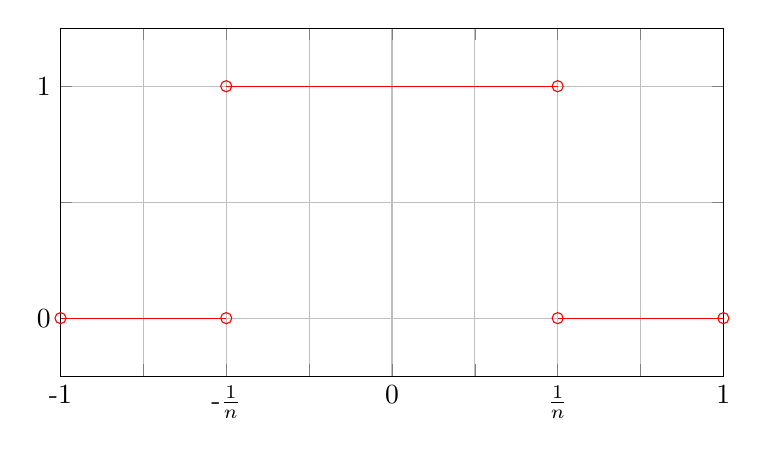
\begin{tikzpicture}
         \begin{axis}
        [width=10cm, height=6cm, xmin=-1, xmax=1, ymin=-0.25, ymax=1.25, xmajorgrids=true, ymajorgrids=true, xtick={-1,-0.75,-0.5,-0.25,0,0.25,0.5,0.75,1},  xticklabels={-1,,-$\frac{1}{n}$,,0,,$\frac{1}{n}$,,1}, ytick={0,0.5,1}, yticklabels={0,,1}]
        \addplot[color=red, mark=o] coordinates {(-1,0) (-0.5,0)};
        \addplot[color=red, mark=o] coordinates {(-0.5,1) (0.5,1)};
        \addplot[color=red, mark=o] coordinates {(0.5,0) (1,0)};
        \end{axis}
    \end{tikzpicture}
    \caption{Densidad uniforme $(-1/n$, $1/n)$.}
\end{figure}

Sea $f \in C_b(\R)$ una función contínua y acotada, entonces la esperanza $\E(f(X_n))$ está dada por:
\[\E(f(X_n)) = \int_{\R}f(x)\mu_n(dx)\]
Donde $\mu_n(dx)$ está dado por la densidad de la distribución de $X_n$, es decir la uniforme:\\ $\mu_n(dx) = \frac{n}{2} \mathbbm{1}_{(-\frac{1}{n},\frac{1}{n})}(x)dx$. Luego:
\[\E(f(X_n)) = \int_{\R}f(x)\,\frac{n}{2}\mathbbm{1}_{(-\frac{1}{n},\frac{1}{n})}(x)dx = \frac{n}{2}\int_{-\frac{1}{n}}^{\frac{1}{n}}f(x)dx\]
Haciendo uso del \textbf{teorema del valor medio} en integrales y de la continuidad de $f$, sabemos de la existencia de un valor $\xi_n \in (-\frac{1}{n},\frac{1}{n})$ tal que la integral anterior es de la forma:
\[\int_{-\frac{1}{n}}^{\frac{1}{n}}f(x)dx = \frac{2}{n}f(\xi_n)\]
Así,
\[\E(f(X_n)) = \frac{n}{2}\int_{-\frac{1}{n}}^{\frac{1}{n}}f(x)dx = f(\xi_n)\]
Por lo tanto la convergencia de $\E(f(X_n))$ estará dad por la convergencia de la nueva sucesión de puntos $(\xi_n)_{n\in\N}$. Para ver la convergencia de $\xi_n$ notemos que:
\begin{itemize}
    \item $\forall\,m\leq n$: $\left(-\frac{1}{n},\frac{1}{n}\right)\subset \left(-\frac{1}{m},\frac{1}{m}\right)$, por lo tanto:
    \[\xi_n \in \bigcap_{m=1}^{n}\left(-\frac{1}{m},\frac{1}{m}\right)\]
    Así la sucesión $\xi_n$ es acotada.
    \item Luego, la sucesión tiene al menos un punto de acumulación. Supongamos que $\Bar{\xi}$ es punto de acumulación de $(\xi_n)_n$, por lo dicho anteriormente debería suceder que:
    \[\Bar{\xi} \in \bigcap_{n\geq 1}\left(-\frac{1}{n},\frac{1}{n}\right) = \{0\}\]
    Finalmente se deduce que $\Bar{\xi}=0$.
\end{itemize}
Nuevamente, aplicando la continuidad de $f$:
\[\E(f(X_n)) = f(\xi_n) \rightarrow\,f(0) = \langle \delta_{0},f\rangle = \E(f(0))\]
\newpage
Así concluímos que:
\begin{itemize}
    \item $\mu_n \Rightarrow\,\delta_{0}$, donde $\mu_n$ estaba dada por las distribuciones uniformes.
    \item $X_n \xrightarrow{\mathcal{L}}\,X$, donde $X\equiv 0$.
\end{itemize}
\end{ejemplo}

\begin{ejemplo}
    Nuevamente tomamos como ejemplo $E=\R$, y definimos la siguiente medida:
    \[\mu_n = \frac{1}{n+1}\sum_{k=0}^{n}\delta_{k/n}\]
    De forma alternativa, definiendo $\mu_n = \mathcal{L}(X_n)$, donde $X_n$ corresponde al experimento de escoger un valor al azar del conjunto $\{0,\frac{1}{n},\frac{2}{n},\cdots,\frac{n}{n}\}$ y sea $\mu = \mathcal{L}(X)$, con $X\sim unif(0,1)$. Entonces $\forall$ $f\in C_b(\R)$:
    \[\langle \mu_n ,f\rangle = \frac{1}{n+1}\sum_{k=0}^{n} \langle \delta_{k/n},f\rangle = \frac{1}{n+1}\sum_{k=0}^{n}f(k/n)\]
    Notando que, para cada $n\in\N$ el conjunto $\{\frac{k}{n}\,|\,k=0,\cdots,n\}$ representa un refinamiento del intervalo $[0,1]$ y $f$ es una función acotada y contínua en ese intervalo (por lo tanto es \textit{Riemann-integrable}), entonces la suma anterior converge por ser suma de riemann, y:
    \[\langle \mu_n ,f\rangle = \frac{1}{n+1}\sum_{k=0}^{n}f(k/n) \xrightarrow{n\rightarrow\infty}\, \int_{0}^{1}f(x)dx = \langle \mu,f\rangle\]
    Luego $\mu_n \Rightarrow\,\mu$, i.e. $X_n \xrightarrow{\mathcal{L}}\,X$.
\end{ejemplo}
\subsubsection{El Teorema Portmanteau}
El siguiente teorema nos proporciona útiles equivalencias a la convergencia débil; cada una de ellas sirve como una definición. Un conjunto $A \in \mathcal{B}(E)$ cuya frontera $\partial A$ satisfaga que $\mu(\partial A) = 0$ se dirá conjunto \textit{$\mu$-contínuo} (Note que $\partial A$ es cerrado, por lo tanto pertenece a $\mathcal{B}(E)$).
\begin{teorema}[Portmanteau] Sean $\mu_n,\mu \in \mathcal{P}(E)$. Las siguientes propociciones son equivalentes:
\begin{itemize}
    \item[i)] $\mu_n \Rightarrow \mu$
    \item[ii)] $\langle \mu_n,f\rangle \rightarrow\, \langle \mu, f\rangle$ para toda función $f$ acotada y uniformemente contínua.
    \item[iii)] $\langle \mu_n , f \rangle \rightarrow\, \langle \mu, f\rangle$ para toda función $f$, Lipschitz.
    \item[iv)] $\limsup_n \mu_n(F) \leq \mu(F)$   $\forall F \subset E$ cerrado.
    \item[v)] $\liminf_n \mu_n(G) \geq \mu(G)$     $\forall G\subset E$ abierto.
    \item[vi)] $\lim\, \mu_n(A) = \mu(A)$ para todo $A$, conjunto \textit{$\mu$-contínuo}. 
\end{itemize}
\end{teorema}
Notemos que, en el caso del \textbf{Ejemplo 1}, la desigualdad del punto $iii)$ se satisface estrictamente si $F=\{0\}$, de la misma forma en el punto $iv)$ si $G=\{0\}^{c}$. Si tomamos $A=\{0\}$, la convergencia no se alcanza en el punto $vi)$, pero esto no contradice el teorema, ya que la medida límite de $\partial \{0\} = \{0\}$ es 1, no 0. 
\\ \newline
\textbf{Demostración (Portmanteau):} Dado que las funciones uniformemente contínuas, en particular son contínuas, la implicancia $i)\rightarrow ii)$ se desprende trivialmente de la definicion de convergencia débil en $i)$. Así mismo la implicancia $ii) \rightarrow iii)$ considerando las funciones Lipschitz.\\
Veamos la implicancia $iii) \rightarrow iv)$: \\ \newline
Sea $F$ un conjunto cerrado. $\forall \epsilon > 0$, sea:
\begin{equation}
   f(x) = \max\left(1-\frac{d(x,F)}{\epsilon}, 0\right)
   \label{eq:dem1}
\end{equation}

Donde $d(x,F)$ está dado por la métrica del espacio $E$. Se puede probar que la función $f$ definida de esta forma es $\frac{1}{\epsilon}$-Lipschitz y vale 1 en todo $F$. Además:
\begin{equation}
    \mathbbm{1}_F \leq f \leq \mathbbm{1}_{F^{\epsilon}}\hspace{1cm}\text{donde }F^{\epsilon}:=\{x\in E\,|\,d(x,F)<\epsilon\}\
    \label{eq:demostracionprtmanteau}
\end{equation}
Luego, integrando (bajo $\mu_n$) en las dos primeras partes de la desigualdad y aplicando límite superior:
\[\limsup\,\mu_n(F)\leq \limsup\,\langle \mu_n,f\rangle\]
Pero, como habíamos dicho, al ser $f$ una función Lipschitz, por la proposición $iii)$; $\langle \mu_n,f\rangle$ converge, por lo tanto el límite superior en realidad es el límite, más aún, converge en términos de $\mu$:
\begin{equation}
    \limsup \langle \mu_n,f\rangle = \lim \langle\mu_n,f\rangle = \langle \mu,f\rangle
\end{equation}
Ahora, nuevamente por la expresión en \ref{eq:demostracionprtmanteau}, integrando la segunda desigualdad (ahora bajo $\mu$):
\[\langle\mu,f\rangle \leq \mu(F^{\epsilon})\]
En resumen, tenemos que:
\[\limsup\,\mu_n(F) \leq \langle\mu,f\rangle \leq\mu(F^{\epsilon})\]
Al ser $F$ cerrado y $F^{\epsilon} \searrow F$, por continuidad de la medida se tiene que $\mu(F^{\epsilon})\searrow \mu(F)$ al momento que $\epsilon \rightarrow 0$ concluyendo el resultado.

\begin{figure}
\centering
    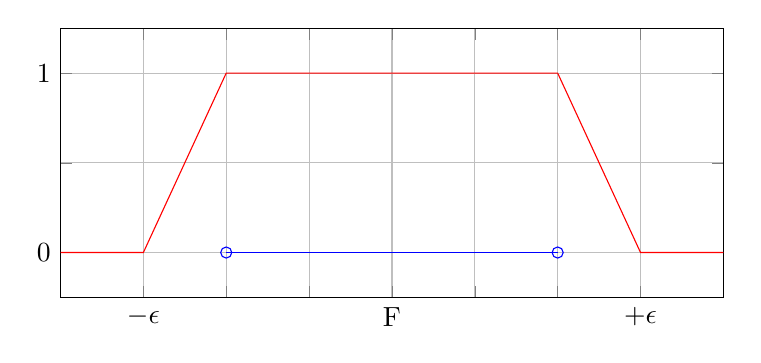
\begin{tikzpicture}
         \begin{axis}
        [width=10cm, height=5cm, xmin=-1, xmax=1, ymin=-0.25, ymax=1.25, xmajorgrids=true, ymajorgrids=true, xtick={-1,-0.75,-0.5,-0.25,0,0.25,0.5,0.75,1},  xticklabels={,$-\epsilon$,,,F,,,$+\epsilon$,}, ytick={0,0.5,1}, yticklabels={0,,1}]
        \addplot[color=red] coordinates {(-1,0) (-0.75,0) (-0.75,0) (-0.5,1) (-0.5,1) (0.5,1) (0.5,1) (0.75,0) (0.75,0) (1,0)};
        \addplot[color=blue, mark = o] coordinates {(-0.5,0) (0.5,0)};
        \end{axis}
    \end{tikzpicture}
    \caption{Esquema función f en \ref{eq:dem1}}
\end{figure}
\newline
Es directo ver que la proposición $iv)$ y $v)$ son equivalentes, así que la implicancia $iv) \rightarrow v)$ es directa de tomar complemento y utilizar que $\mu_n$ y $\mu$ son medidas de probabilidad.\\ \newline
Veamos que $iv)\land v)$ implican a $vi)$: Sea $A$ un conjunto $\mu$-contínuo. Dado que $\Bar{A}$ es cerrado, $A^{\circ}$ es abierto, ocupando la proposición $iv)$ y $A^{\circ} \subset A\subset \Bar{A}$:
\[\mu(\Bar{A}) \geq \limsup\,\mu_n(\Bar{A}) \geq \limsup\,\mu_n(A)\geq \liminf\,\mu_n(A) \geq \liminf\,\mu_n(A^{\circ})\geq \mu(A^{\circ})\]
Además, como $A$ es $\mu$-contínuo: $\mu(\partial A) = 0$, entonces $\mu(\Bar{A}) = \mu(A^{\circ}) = \mu(A)$, por lo tanto todas las desigualdades anteriores son, en realidad, igualdades. Concluímos así que:
\begin{itemize}
    \item $\liminf\,\mu_n(A) = \limsup\,\mu_n(A)$ por lo tanto el límite existe.
    \item $\mu(A)\geq \lim\,\mu_n(A)\geq \mu(A)$, por lo tanto $\lim\,\mu_n(A) = \mu(A)$.
\end{itemize}
Por último, para finalizar, veremos la implicancia $vi)\rightarrow i)$:\\ \newline
Sea $f\in C_b(E)$, sin pérdida de generalidad podemos suponer que $0\leq f\leq 1$. En caso contrario, como $f$ es una función acotada, su supremo e ínfimo son finitos, por lo tanto podríamos definir una normalización para $f$:
\[\Tilde{f} = \frac{f - \inf_x f}{\sup_x f - \inf_x f}\]
Para la siguiente demostración haremos uso del siguiente resultado:
\begin{lem} Sea $g$ una función positiva, entonces:
    \begin{equation}
        \E_{\mu}(g(X)) = \langle\mu,g\rangle = \int_0^{\infty}\mu(g>t)dt
    \end{equation}
\end{lem}
\textbf{Demostración (Lema 1):} La primera igualdad es la definición de esperanza:
\[\E_{\mu}(g(X)) = \int_{0}^{\infty}g(x)\mu(dx)\]
Al mismo tiempo, podemos reescribir la función $g$ de la forma:
\[\E_{\mu}(g(X)) = \int_{0}^{\infty}\left(\int_{0}^{g(x)}dt\right)\,\mu(dx)\]
Ahora podemos extender la integral en $dt$ a todo el intervalo positivo mediante una indicatriz que anule los valores superiores a $g(x)$, esto es:
\[\E_{\mu}(g(X)) = \int_{0}^{\infty}\left(\int_{0}^{\infty}\mathbbm{1}_{\{g>t\}}dt\right)\mu(dx) = \int_{0}^{\infty}\int_{0}^{\infty}\mathbbm{1}_{\{g>t\}}dt\mu(dx)\]
Ocupando el teorema de Fubini podemos intercambiar el orden de las integrales, entonces:
\[\E_{\mu}(g(X)) = \int_{0}^{\infty}\int_{0}^{\infty}\mathbbm{1}_{\{g>t\}}dt\mu(dx) = \int_{0}^{\infty}\int_{0}^{\infty}\mathbbm{1}_{\{g>t\}}\mu(dx)dt \]
\[ = \int_{0}^{\infty}\mu(g>t)dt\]
\rule{0.7em}{0.7em}

Entonces, volviendo a la demostración del teorema, tenemos que:
\[\langle \mu,f\rangle = \int_{0}^{1}\mu(f>t)dt\]
\[\langle \mu_n , f \rangle = \int_{0}^{1}\mu_n(f>t)dt\]
Donde el intervalo de integración lo podemos acotar, puesto que definimos el rango de la función $f$ en $[0,1]$. Además, como $f$ es contínua, es fácil ver que:
\[\partial \{f>t\} \subset\,\{f=t\}\]
Notemos que $\mu(f=t)=0$ salvo para, a lo más numerables, valores de t's. De lo contrario, la medida $\mu$ no sería finita. Luego, $dt-c.s.$ tenemos:
\[\mu(\partial\{f>t\}) \leq \mu(\{f=t\}) = 0\]
Es decir: de manera $dt-c.s.$ $\{f>t\}$ es $\mu$-contínuo. Por la proposición $vi)$:
\[\mu_n(f>t) \xrightarrow{\,\,n\,\,}\,\mu(f>t)\hspace{1cm}dt-c.s.\]
Finalmente, ocupando el \textbf{T.C.D.}:
\[\langle\mu_n,f\rangle = \int_{0}^{\infty}\mu_n(f>t)dt \xrightarrow{\,\,\,\textbf{T.C.D.}\,\,\,}\int_{0}^{\infty}\mu(f>t)dt = \langle \mu,f\rangle\]
\rule{0.7em}{0.7em}

Habiendo establecido anteriormente, la equivalencia entre la convergencia débil de medidas de probabilidad y la convergencia en LEY de variables aleatorias, podemos enunciar el Teorema Portmanteau para variables aleatorias.

\begin{teorema}[Portmanteau para variables aleatorias.] Sean $(X_n)_{n\in\N}$, $X$ variables aleatorias en $(E,d)$ espacio métrico. Las siguientes proposiciones son equivalentes:
\begin{enumerate}
    \item[i)] $X_n\,\xrightarrow{\mathcal{L}}\,X$
    \item[ii)] $\E(f(X_n)) \xrightarrow{\,\,n\,\,}\E(f(X))$ para toda función $f$ acotada y uniformemente contínua.
    \item[iii)] $\E(f(X_n)) \xrightarrow{\,\,n\,\,}\E(f(X))$ para toda función $f$ Lipschitz.
    \item[iv)] $\limsup\,\pb(X_n \in F) \leq \pb(X\in F)$ $\forall F\subset E$ cerrado.
    \item[v)] $\liminf\,\pb(X_n \in G) \geq \pb(X \in G)$ $\forall G\subset E$ abierto.
    \item[vi)] $\lim \pb(\X_n \in A) = \pb(X\in A)$ para todo $A\in \mathcal{B}(E)$ conjunto $\mu$-contínuo ( $\pb(X \in \partial A) = 0$ ).
\end{enumerate}
\end{teorema}

\begin{obs} Tomando $E=\R$, la condición $vi)$ del teorema suele ser interesante, como en el siguiente ejemplo:\\ Sabemos de ejemplos anteriores que:
\[\delta_{1/n}\Rightarrow \,\delta_{0}\]
Sin embargo, para el conjunto $A=(0,\infty)$, $\forall\,n\in\N$:
\[\delta_{1/n}(A) = 1\]
\[\delta_{0}(A) = 0\]
Es decir que $\delta_{1/n}(A)$ no converge a $\delta_{0}(A)$, sin embargo esto no contradice la condición $vi)$, pues el conjunto $A$ no es $\delta_0$-contínuo.
\[\delta_{0}(\partial A) = \delta_{0}(\{0\}) = 1\]
\end{obs}

\subsubsection{El Teorema del Mapeo.}
Supongamos que $h$ es una función de $(E,d)$ a otro espacio métrico, $(\hat{E},\hat{d})$. \\Si $h$ es $\mathcal{B}(E)/\mathcal{B}(\hat{E})$-medible, entonces cada medida de probabilidad $\mu \in \mathcal{P}(E)$ induce a otra medida de probabilidad $\mu h^{-1} \in \mathcal{P}(\hat{E})$, definida de la manera usual, como $\mu h^{-1}(A) = \mu(h^{-1}(A))$. \\ \newline
Necesitamos, entonces, condiciones bajo las cuales el hecho de tener una convergencia débil, $\mu_n \Rightarrow \mu$, en $\mathcal{P}(E)$, me implique una convergencia débil, $\mu_nh^{-1} \Rightarrow \mu h^{-1}$ para medidas en $\mathcal{P}(\hat{E})$. \\ \newline
Una de las condiciones pensadas para $h$ podrías ser la continuidad, pero veremos que esta condición puede ser reemplazada por una más débil. Asumimos que $h$ será una función $\mathcal{B}(E)/\mathcal{B}(\hat{E})$-medible, y sea $D_h$ el conjunto de los puntos de discontinuidad de la función $h$ ($D_h \in \mathcal{B}(E)$). Tenemos el siguiente resultado;  si $\mu_n \Rightarrow\,\mu$ y $\mu(D_h) = 0$, entonces $\mu_n h^{-1} \Rightarrow\, \mu h^{-1}$. \\ \newline
En otras palabras:

\begin{teorema}[Del Mapeo.] Sea $(\hat{E},\hat{d})$ otro espacio métrico y sea $h:\,E\rightarrow\,\hat{E}$, una función medible. $(X_n)_{n\in\N}$, $X$ son variables aleatorias en $E$.\\ \newline
Si $X_n\,\xrightarrow{\mathcal{L}}\,X$ y $\pb(X \in D_h) = 0$, entonces: $h(X_n) \,\xrightarrow{\mathcal{L}}\,h(X)$. Donde $D_h :=\{x\in E\,|\,\text{$h$ es discontínua en x}\}$
\end{teorema}

\textbf{Demostración:} Sea $B \subset\,\hat{E}$, un conjunto $\mathcal{L}(h(X))$-contínua, es decir:
\begin{equation}
    \pb(h(X) \in \partial B) = 0
    \label{eq:dem2}
\end{equation}
Por el teorema Portmanteau en variables aleatorias, la convergencia el LEY es equivalente a decir que:
\[\pb(h(X_n)\in B) \xrightarrow{\,\,n\,\,}\,\pb(h(X)\in B)\]
Lo que a su vez, es equivalente a decir que:
\[\pb(X_n \in h^{-1}(B)) \xrightarrow{\,\,n\,\,}\,\pb(X \in h^{-1}(B))\]
Luego, basta con demostrar que $h^{-1}(B)$ es un conjunto $\mathcal{L}(X)$-contínuo, $i.e.$; falta por demostrar que $\pb(X \in \partial h^{-1}(B)) =0$.\\ \newline
Sea $x \not\in D_h$, luego:
\[\text{si }x\in\overline{h^{-1}(B)}\,\Rightarrow\,\exists\,x_n \in h^{-1}(B)\,\text{tal que }x_n\,\rightarrow\,x\]
\[\Rightarrow\,h(x)\in\,\overline{B}\]
Similarmente, si $x\not\in\,D_h$,
\[\text{si }x\in\,int\left(h^{-1}(B)\right)^{c}\,\Rightarrow\,\exists\,x_n \rightarrow\,x\,\text{ tal que  }x_n\,\not\in\,h^{-1}(B)\]
\[i.e:\hspace{0.2cm}h(x_n)\not\in\,B^{\circ}\]
Luego, para $x\not\in D_h$:
\[x\,\in\,\patial h^{-1}(B) \,\Rightarrow\,h(x)\in\partial B\,\hspace{1cm}\text{Es decir:}\]
\[\partial h^{-1}(B) \cap D_h^{c}\,\,\subset\,h^{-1}(\partial B)\cap D_h^{c}\,\,\subset\,h^{-1}(\partial B)\]
Así, y dado el hecho de que $D_h^{c}$ es un conjunto de medida $1$:
\[\pb(X \in \partial h^{-1}(B)) = \pb(X \in \partial h^{-1}(B) \cap D_h^{c}) \leq \pb(X \in h^{-1}(\partial B))=0\]
De donde la última igualdad se tiene por la hipótesis $\ref{eq:dem2}$.
\rule{0.7em}{0.7em}

\begin{obs}
La convergencia en ley de $X_n$ a $X$ no requiere que los $X_n$ y $X$ estén definidos en el mismo espacio de probabilidades, puesto que para cada $n\in\N$ el espacio $(\Omega,\mathcal{F},\mu_n)$ va cambiando de medida, a diferencia de la convergencia $c.s.$ o en probabilidad.
\end{obs}

\begin{prop}
Sean $(X_n)_{n\in\N}$ y $X$ variables aleatorias definidas sobre el mismo espacio de probabilidades. Entonces:
\[X_n\xrightarrow{\,\,c.s.\,\,} X \Rightarrow\,X_n \xrightarrow{\,\,\pb\,\,}X \Rightarrow\,X_n\,\xrightarrow{\,\,\mathcal{L}\,\,}X\]
\end{prop}
\textbf{Demostración: propuesto.}\\ \newline

\subsection{Tensión (Tightness)}
\subsubsection{Relativamente compacto.}
Sea $M\subset \mathcal{P}(E)$ una familia de medidas de probabilidad sobre el espacio métrico $(E,d)$. Diremos que $M$ es \textit{relativamente compacto} si cada sucesión de elementos en $M$ contiene una subsucesión que converge débilmente, es decir; si $\{\mu_n\}$ es una secuencia de elementos en $M$, entonces existe una subsucesión $\{\mu_{n_i}\}$ y una medida de probabilidad $\mu \in \mathcal{P}(E)$, tal que $\mu_{n_i} \Rightarrow \mu$.  \\ \newline
Notamos que esta caracterización evita la descripción topológica que se encuentra subyacente en las definiciones de \textit{compacidad} o \textit{convergencia}. Se puede mostrar la existencia de una métrica que dota al espacio de tal topología pero no es de vital importancia para este curso, he ahí el motivo de su ausencia en estas notas. \\ \newline
Sin embargo, notamos que esta definición genera cierto problema para probar que un conjunto de medidas es relativamente compacto, dada la escasa gama de herramientas que poseemos en este momento. Es por esto, que se introduce la siguiente definición:

\begin{definicion}[Tensión] Una familia $M\subseteq \mathcal{P}(E)$ se dice \textbf{TENSA} si $\forall \epsilon > 0$, $\exists K\subseteq E$ compacto tal que:
\[\mu(K) > 1-\epsilon \hspace{1cm}\forall\,\mu\in M\]
\end{definicion}
\\ \newline
El siguiente resultado importante justifica la definición anterior:


\begin{teorema}[de Prohorov] Sea $M\subseteq \mathcal{P}(E)$.
\begin{itemize}
    \item[i)] Si $M$ es tensa, entonces es relativamente compacta.
    \item[ii)] Supongamos que $E$ es un espacio \textbf{polaco} (espacio métrico completo y separable). Si $M$ es relativamente compacta, entonces es tensa.
\end{itemize}
\end{teorema}

\begin{cor} Si $\{\mu_n\}$ es tensa y cada subsucesión débilmente convergente, converge a la misma medida $\mu\in\mathcal{P}(E)$, entonces toda la secuencia $\mu_n$ converge débilmente a $\mu$: $\mu_n \Rightarrow \mu$.
\end{cor}
\textbf{Demostración:} Ver \cite[págs. 59,69]{Bill}
\begin{ejemplo}
\begin{itemize}
    \item Si $E$ es compacto, entonces toda familia $M\subseteq \mathcal{P}(E)$ es tensa.
    \item En $E=\R$, sea $M=\{\delta_n \}$ el conjunto de las delta de Dirac en los puntos $n\in\N$. Claramente $M$ no es tensión, cada vez que proponemos un conjunto compacto, al ser la sucesión \\$\{n\,|\, n\in\N\}$ no acotada, existirá un $n$ suficientemente grande que se escape del compacto en $\R$. 
    \item En $E=\R$, sea $M=\{\mathcal{N}(0,n)\}_{n\in\N}$. $M$ no es tensión.
\begin{figure}[h!]
\centering
    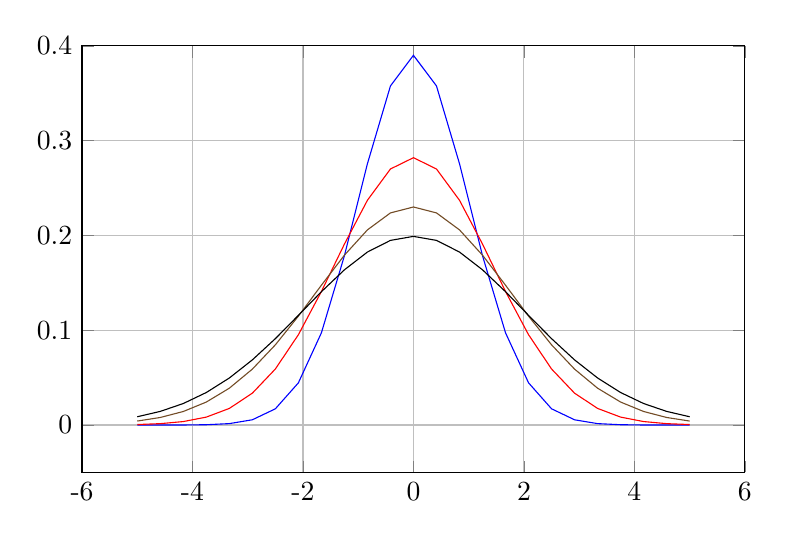
\begin{tikzpicture}
         \begin{axis}
        [width=10cm, height=7cm, xmin=-6, xmax=6, ymin=-0.05, ymax=0.4, xmajorgrids=true, ymajorgrids=true, xtick={-6,-4,-2,0,2,4,6},  xticklabels={-6,-4,-2,0,2,4,6}, ytick={0,0.1,0.2,0.3,0.4}, yticklabels={0,0.1,0.2,0.3,0.4}]
        
        \addplot+[no marks]{0.39*e^(-0.5*x^2)};
        \addplot+[no marks]{0.282*e^(-0.25*x^2)};
        \addplot+[no marks]{0.23*e^(-0.16*x^2)};
        \addplot+[no marks]{0.199*e^(-0.125*x^2)};
        \end{axis}
    \end{tikzpicture}
    \caption{Sucesión de densidades $\mathcal{N}(0,n)$.}
\end{figure}

    \item Sin embargo, considerando $E=\overline{\R}:=\R\cup \{-\infty ,+\infty\}$, entonces la sucesión $M=\{\delta_n \}_n$ es tensa pues: $\delta_n \Rightarrow \delta_{+\infty}$.
    
    \item De la misma forma, si $E=\overline{\R}$, la familia de medidas $M=\{\mathcal{N}(0,n)\}_n$, entonces:
    \[\mathcal{N}(0,n) \Rightarrow\,\frac{1}{2}\,\delta_{-\infty} + \frac{1}{2}\,\delta_{+\infty}\]
\end{itemize}
\end{ejemplo}

\section{Función Característica}
Son variadas las transformaciones o funciones generadoras usadas en matemáticas, probabilidades y estadística. En general, todas ellas se basan en el uso de la función exponencial y su ventaja de convertir sumas en productos. En la siguiente sección se denotará como $i$ $(=\sqrt{-1})$ a la componente imaginaria de un valor complejo.\\
Los siguientes son ejemplos de transformadas o funciones del tipo antes mencionado:
\begin{enumerate}
    \item Función generadora de probabilidades: $g(s)=\E(s^{X})$
    \item Función generadora de momentos: $m(t) = \E(e^{tX})$
    \item Transformada de Laplace: $\mathbb{L}(t) = \E(e^{-tX}) = \int e^{-tx}\mu(dx)$
    \item Transformada de Fourier: $\E(e^{-itX}) = \int e^{-itx}\mu(dx)$
\end{enumerate}

En lo que sigue, nuestro espacio de trabajo será el espacio métrico $\R$ o $\R^{d}$ dotados de las métricas usuales.

\begin{definicion}[Función Característica] Dada $\mu \in \mathcal{P}(\R^{d})$, definimos su FUNCION CARACTERÍASTICA como:

    \[\hat{\mu}:\,\R^{d} \longrightarrow\,\C\]
    \begin{equation}
    t \longrightarrow \hat{\mu}(t) := \int_{\R^d} e^{it\cdot x}\mu(dx)
\end{equation}
Donde la notación:
\[t\cdot x = \sum_{j=1}^{d}t_j x_j\]
\end{definicion}

Equivalentemente, podemos enunciar la definición anterior para variables aleatorias, donde la función característica de la variable está dada por la función característica de su ley.

\begin{definicion} Dada $X$, variable aleatoria en $\R^d$, su FUNCIÓN CARACTERÍSTICA es:
\[\varphi_X(t):\R^d \longrightarrow\,\C\]
\begin{equation}
    t \,\longrightarrow\,\varphi_X(t) := \E(e^{it \cdot X})
\end{equation}
\end{definicion}
\begin{obs} Podemos notar que la función característica toma valores en el plano complejo, sin embargo; su cálculo se efectúa sólamente en variables reales.
\[\varphi_X(t) = \E(e^{itX}) = \int e^{itx}\mu(dx) = \E(cos(tX)) + i\,\E(sen(tX))\]
\end{obs}

\begin{ejemplo}
 $X\sim \mathcal{N}(\mu,\sigma^{2})$, donde, en este caso, $\mu$ y $\sigma$ son valores reales. Entonces:
 \[\varphi_X(t) = e^{i\mu t -\frac{\sigma^2 t^2}{2}}\]
\end{ejemplo}

La gran ventaja de la función característica por sobre las funciones como la transformada de Laplace, la funciones generadora de probabilidades o la función generadora de momentos es que garantiza la existencia de la esperanza en cualquier medida de probabilidad. Ya que, todo el cálculo se realiza al integrar sobre una función acotada; $|e^{itx}|\leq 1$ para todo valores $x,t \in \R$. Las siguientes proposiciones serán enunciadas para $\R$ pero son ciertas en $\R^d$.

\begin{prop} Sea $X$ variable aleatoria, $\varphi = \varphi_X$. Entonces:
\begin{itemize}
    \item[i)] $\varphi$ existe $\forall\,t$ y para cualquier distribución de $X$.
    \item[ii)] $\varphi(0)=1$
    \item[iii)] $|\varphi(t)|\leq 1$ para todo $t$
    \item[iv)] $\varphi$ es uniformemente contínua, esto es; $\forall\,\epsilon >0$, existe $\delta >0$ tal que, $|\varphi(t)-\varphi(s)|\leq \epsilon$, para cualesquiera $t, s$ tales que $|t-s|\leq \delta$
    \item[v)] $\varphi_{a +bX}(t) = e^{iat}\varphi(bt)$, para todos $a,b\in\R$.
    \item[vi)] la función característica de $-X$ es el valor conjugado de $\varphi$, esto es; $\varphi_{-X}(t) = \overline{\varphi(t)}$
    \item[vii)] Si $\varphi(t)\in \R\,\,\forall\,t$ $\Longleftrightarrow$ $\mathcal{L}(X) = \mathcal{L}(-X)$
\end{itemize}
\end{prop}

\textbf{Demostración (proposición):}
\begin{itemize}
    \item[i)] Notemos que para cualquier $x$ o $t$, la función $|e^{itx}|\leq 1$. Dado que las medidas de probabilidades son finitas, luego la función $e^{itx}$ siempre es integrable.
    
    \item[ii)] Si $t=0$, entonces $e^{itx} = 1$, luego $\E(e^{0})= 1$.
    \item[iii)] 
    \[|\varphi(t)| = |\E(e^{itX})| = \left| \int_{\R}e^{itx}\mu(dx) \right|\]
    \[\leq \int_{\R}|e^{itx}| \mu(dx) \leq 1\cdot \mu(\R) \leq 1\]
    \item[iv)] Sea $h=t-s$, asumimos sin pérdida de generalidad $s<t$. Entonces:
    \[|\varphi(t) -\varphi(s)| = |\E(e^{itX})-\E(e^{isX})| = |\E(e^{i(h+s)X})-\E(e^{isX})|\]
    \[\leq |\E(e^{isX}(e^{ihX}-1))|\leq \E(|e^{isX}|\cdot |e^{ihX}-1|)\]
    \[\leq \E(|e^{ihX}-1|)\]
    Cuando $h\rightarrow 0$, la función $e^{ihX}-1$ converge a $0$ para todo $\omega \in \Omega$. Es decir, $e^{ihX}-1 \xrightarrow{h\rightarrow 0} 0$ $c.s.$, como además esta función está acotada por 2 para cualquier valor de $t$ o $X$, ocupando el \textbf{T.C.D.} concluímos que:
    \[\lim_{h\to 0}\E(e^{ihX}-1) = 0\]
    
    \item[v)] Por definición:
    \[\varphi_{a+bX}(t) = \E(e^{it(a+bX)}) = \E(e^{iat}e^{i(bt)X}) = e^{iat}\E(e^{i(bt)X}) = e^{iat}\varphi(bt)\]
    \item[vi)] Recordamos que el conjugado del complejo $a+ib$ es $a-ib$. Entonces:
    \[\E(e^{it(-X)})= \E(cos(-tX)+isen(-tX)) = \E(cos(tX)-isen(tX))= \E(cos(tX))-i\,\E(sen(tX)) = \overline{\varphi(t)}\]
\item[vii)] $(\Leftarrow)$ Como $\varphi$ está dado por la ley de la variable, tenemos que:
\[\mathcal{L}(X)=\mathcal{L}(-X) \Rightarrow\,\varphi_X(t) = \varphi_{-X}(t)\]
Pero, por lo mostrado en el punto $iv)$, concluímos que $\varphi(t) = \overline{\varphi(t)}$ $\forall\,t$ y eso sólo pasa cuando la función toma valores reales.\\ \newline
Para la implicancia $(\Rightarrow)$ hemos de necesitar resultados posteriores y se mostrará más adelante.
\end{itemize}
\rule{0.7em}{0.7em}

Otra de las propiedades interesantes que posee la función característica tiene que ver con la medida de probabilidad generada por la convolución de medidas.

\begin{definicion} Dadas $\mu,\nu \in \mathcal{P}(\R)$, su convolución $\mu\ast \nu \in \mathcal{P}(\R)$, se define como:
\[\int f(z)\mu\ast\nu(dz) = \int\int f(x+y)\mu(dx)\nu(dy)\hspace{0.7cm}\forall\,f\,\text{medible}\]
\end{definicion}
\begin{prop}$\forall\,\mu,\nu\,\in\mathcal{P}(\R)$:
\[\widehat{\mu\ast\nu}(t) = \hat{\mu}(t)\hat{\nu}(t)\]
Equivalentemente, si $X\amalg Y$, son variables aleatorias en $\R$:
\[\varphi_{X+Y}(t) = \varphi_X(t)\varphi_Y(t)\hspace{1cm}\forall\,t\]
\end{prop}

El principal interes en la función característica es que describe de manera única a las distribuciones. Las probabilidades de intervalos se pueden recuperar mediante la función característica gracias al siguiente teorema de inversión.

\begin{teorema}[Fórmula de Inversión.] Sea $X$ una variable aleatoria en $\R$, Para todo $a<b$ se tiene que:
\[\pb(a<X<b) + \frac{\pb(X=a)+\pb(X=b)}{2} = \lim_{T\to \infty}\frac{1}{2\pi}\int_{-T}^{T}\frac{e^{-ita}-e^{-itb}}{it}\varphi_X(t)dt\]
\end{teorema}
\textbf{Demostración (fórmula de Inversión):} Sea $\mu = \mathcal{L}(X)$. Denotemos por $I_T$ a la siguiente integral:
\[I_T = \int_{-T}^{T}\frac{1}{2\pi}\frac{e^{-ita}-e^{-itb}}{it}\varphi_X(t) dt\]
Reemplazamos la definición de función característica:
\[I_T = \int_{-T}^{T}\frac{e^{-ita}-e^{-itb}}{2\pi it}\int_{\R}e^{itx}\mu(dx) dt = \int_{\R}\int_{-T}^{T}\frac{e^{-ita}-e^{-itb}}{2\pi it}e^{itx}dt\mu(dx)\]
Usando la identidad de Euler para números complejos; $e^{i\alpha} = cos(\alpha)+i\,sin(\alpha)$, tenemos que:
\[I_T = \int_{\R}\int_{-T}^{T}\left(\frac{cos(t(x-a))-cos(t(x-b))}{2\pi it} + i\,\frac{sin(t(x-a))-sin(t(x-b))}{2\pi it}\right)dt \mu(dx)\]
Usando que la función \textit{coseno} es una función par, y la función identidad es impar, tenemos que la expresión:
\[\frac{cos(t(x-a))-cos(t(x-b))}{t}\]
es una función impar para la variable $t$, por lo tanto; toda integral sobre un intervalo simétrico es nula.
\[\frac{1}{2\pi i}\int_{-T}^{T}\frac{cos(t(x-a))-cos(t(x-b))}{t} dt = 0\]
Del mismo modo, la función \textit{seno} y la función identidad son funciones impares, por lo tanto la expresión:
\[\frac{sin(t(x-a))-sin(t(x-b))}{t}\]
es una función par, por lo tanto; para toda integral sobre un intervalo simétrico, tenemos que:
\[\frac{1}{2\pi i}\int_{-T}^{T}\frac{sin(t(x-a))-sin(t(x-b))}{t}dt = \frac{2}{2\pi i}\int_{0}^{T}\frac{sin(t(x-a))-sin(t(x-b))}{t}dt\]
Por lo tanto la integral $I_T$ queda de la siguiente forma:
\[I_T = \int_{\R}\frac{2i}{2\pi i}\int_{0}^{T}\frac{sin(t(x-a))-sin(t(x-b))}{t}dt \mu(dx)=\int_{\R}\left(\frac{1}{\pi }\int_{0}^{T}\frac{sin(t(x-a))-sin(t(x-b))}{t}dt\right) \mu(dx)\]
\[= \int_{\R}\frac{1}{\pi}\left(\int_{0}^{T}\frac{sin(t(x-a))}{t}dt - \int_{0}^{T}\frac{sin(t(x-b))}{t}dt\right) \mu(dx)\]

Para El siquiente paso ocuparemos el siguiente lema:
\begin{lem} Sea $c\in\R$:
\[\lim_{T \to \infty}\frac{1}{\pi}\int_{0}^{T}\frac{sin(ct)}{t}dt = \begin{cases}
                -\frac{1}{2} & si\hspace{0.2cm}c<0\\
                \,\frac{1}{2} & si\hspace{0.2cm}c>0\\
                \,0 & si\hspace{0.2cm} c=0
                \end{cases}\]
\end{lem}
De esta forma, el límite de $I_T$ dependerá de los valores de $x$ respecto a $a$ y $b$ (tomando $c=x-a$ o $c=x-b$). Luego, si $a<b$, tenemos que:
\[\lim_{T\to \infty}\frac{1}{\pi}\left(\int_{0}^{T}\frac{sin(t(x-a))}{t}dt - \int_{0}^{T}\frac{sin(t(x-b))}{t}dt\right) = 0\]
Para todo $x \in (-\infty ,a)\cup (b,\infty)$. Más aún, basta con verificar el signo de $x-a$ o $x-b$ en cada caso para probar que:
\[\lim_{T\to \infty}\frac{1}{\pi}\left(\int_{0}^{T}\frac{sin(t(x-a))}{t}dt - \int_{0}^{T}\frac{sin(t(x-b))}{t}dt\right) = \begin{cases}
\,\frac{1}{2} & si\hspace{0.2cm}x=a\\
\,\frac{1}{2} & si\hspace{0.2cm}x=b\\
\,1 & si\hspace{0.2cm}x\in(a,b)\\
\,0 & si\hspace{0.2cm}x\in(-\infty,a)\cup(b,\infty)
\end{cases}\]
Por lo tanto el límite de $I_T$ se reduce a:
\[\lim_{T\to \infty}I_T = \int_{\R}\lim_{T\to \infty}\frac{1}{\pi}\left(\int_{0}^{T}\frac{sin(t(x-a))}{t}dt - \int_{0}^{T}\frac{sin(t(x-b))}{t}dt\right)\mu(dx)\]
\[= \int_{\{a\}}\frac{1}{2}\mu(dx) + \int_{\{b\}}\frac{1}{2}\mu(dx) + \int_{(a,b)}1\mu(dx) = \mu((a,b)) + \frac{\mu(\{a\})+\mu(\{b\})}{2}\]
\rule{0.7em}{0.7em}

\begin{cor}
Si $X$ e $Y$ son variables aleatorias tales que $\varphi_X(t) = \varphi_Y(t)$ para todo valor de $t$, entonces $\mathcal{L}(X)=\mathcal{L}(Y)$.
\end{cor}

\begin{teorema} Sea $\mu\in\mathcal{P}(\R)$:
\begin{itemize}
    \item Si $\int |x|^n \mu(dx)\,<\,\infty$ para cierto $n\in\N$, entonces $\varphi$ es $n$ veces derivable y:
    \[\varphi^{(n)}(t) =\int (ix)^n e^{itx}dt\]
    En particular se tiene la igualdad: $\varphi^{(n)}(0)=i^n \int x^n \mu(dx)$.
    \item Si $\varphi^{(2n)}(0)$ existe para cierto $n\in\N$, entonces $\int x^{2n}\mu(dx)\,<\,\infty$.
\end{itemize}
\end{teorema}
\textbf{Demostración: propuesto.}\\ \newline
De manera recíproca, conocer la función característica, $\hat{\mu}$, nos proporciona conocimiento acerca de la forma en que la distribución reparte valores sobre el conjunto y, gracias al último teorema, es posible saber el valor de los momentos asociados en caso de existir. El siguiente resultado analiza el comportamiento de la función característica acercándose "a infinito" y vincula la integrabilidad de la función con la existencia de una densidad para $\mu$ con respecto a la medida de Lebesgue.

\begin{teorema}[Transformada de Fourier para la función característica] Sea $\mu\in\mathcal{P}(\R)$, \\$\varphi = \hat{\mu}$. Supongamos la condición:
\[\int_{\R}|\varphi (t)|dt\,<\,\infty\]
Entonces existe $f$, densidad de $\mu$. Es decir; $\mu(dx) = f(x)dx$, y además se tiene que:
\[f(x) = \frac{1}{2\pi}\int_{\R}e^{-itx}\varphi (t) dt\]
\end{teorema}
\textbf{Demostración: }El primer paso para ver la existencia de una densidad es comprobar que la medida de probabilidad $\mu$ es \textit{no atómica}, es decir, que para cada elemento $a\in\R$, la medida del síngleton es cero: $\mu(\{a\})=0$.\\
Usando la fórmula de inversión tenemos que: para $a<b$:
\[\mu((a,b)) + \frac{\mu(\{a\})+\mu(\{b\})}{2} = \lim_{T\to\infty} \frac{1}{2\pi}\int_{-T}^{T}\frac{e^{-ita}-e^{-itb}}{it}\varphi(t)dt\]
Podemos reemplazar la expresión adentro de la integral de la siguiente forma:
\[\frac{e^{-ita}-e^{-itb}}{it} = \int_{a}^{b}e^{-itx}dx\]
Entonces, acotando:
\[\mu((a,b)) + \frac{\mu(\{a\})+\mu(\{b\})}{2} \leq \lim_{T\to\infty} \left|\frac{1}{2\pi}\int_{-T}^{T}\int_{a}^{b}e^{-itx}dx\,\varphi(t)dt\right|\]
\[\leq \lim_{T\to\infty}\frac{1}{2\pi}\int_{-T}^{T}\int_{a}^{b}|e^{-itx}|dx\,\,|\varphi(t)|dt \,=\,(b-a)\cdot \frac{1}{2\pi}\int_{\R}|\varphi(t)|dt\]
Donde la última igualdad se tiene, pues $|e^{-itx}|=1$ para todo valor de $x$ o de $t$. Ahora, como la integral en todo el espacio de $|\varphi|$ es finita, y dada la continuidad de la medida, cuando hacemos tender $b\rightarrow a$:
\[\mu(\{a\}) \leq \lim_{b\to a} (b-a)\cdot \frac{1}{2\pi}\int_{\R}|\varphi(t)|dt = 0\]
Así prbamos que la medida $\mu$ es \textit{no atómica}, y además:
\[\mu((a,b)) = \frac{1}{2\pi}\int_{\R}\frac{e^{-ita}-e^{-itb}}{it}\,\varphi(t)dt\]
\[= \int_{a}^{b}\left(\frac{1}{2\pi}\int_{\R}e^{-itx}\varphi(t)\,dt\right)\,dx\]
En palabras simples: integrando por la medida de Lebesgue, esa función, sobre ese conjunto, recupero la medida del conjunto. Lo que es la definición de densidad.
\rule{0.7em}{0.7em}\\ \newline

Hemos visto que una condición suficiente para la convergencia puntual de medidas de probabilidad en otro elemento de $\mathcal{P}(E)$ es que la sucesión tomada sea \textit{tensa}. Del mismo modo, la convergencia puntual de funciones características de alguna sucesión de medidas $\mu_n$, no necesariamente sería función característica, ni nos entrega información sobre la convergencia de $\mu_n$. El siguiente teorema nos da condiciones bajo las cuales, los hechos anteriores se pueden asegurar.\\ \newline
\begin{teorema}[Continuidad de Lévy] Sea $(\mu_n)_{n\in\N}$ una sucesión en $\mathcal{P}(\R)$:
\begin{itemize}
    \item[i)] Si $\exists\,\mu\in\mathcal{P}(\R)$ tal que $\mu_n\,\Rightarrow\,\mu$, entonces:
    \[\hat{\mu_n}(t)\xrightarrow{\,\,\,n\,\,\,}\,\hat{\mu}(t) \hspace{1cm} \forall \, t \,\in\,\R\]
    \item[ii)] Si $\hat{\mu_n}(t)\rightarrow\,\vatphi(t)$ $\forall\,t\in\R$, para alguna función $\varphi$ contínua en $0$, entonces $\exists\,\mu\,\in\,\mathcal{P}(\R)$ tal que $\varphi = \hat{\mu}$ y $\mu_n \Rightarrow\mu$.
\end{itemize}
\end{teorema}
\\ \newline

\textbf{Demostración:} \begin{itemize}
    \item[i)] Para la demostración de la primera parte, basta notar que la función $f(x) = e^{itx}\,\in\,C_b(\R)$, por lo tanto, por definición de convergencia débil:
    \[\hat{\mu_n}(t) = \E_{\mu_n}(e^{itX}) = \langle \mu_n , f\rangle\,\xrightarrow{\,\,\,n\,\,\,}\langle \mu, f \rangle = \E_{\mu}(e^{itX}) = \hat{\mu}(t)\]
    
    \item[ii)] Si la sucesión $(\mu_n)_n$ fuese relativamente compacta, entonces:
    \begin{itemize}
        \item[\cdot] $\exists\,\mu\in\mathcal{P}(\R)$ y una subsucesión $\{n_i\}_{i \in \N}$ tal que $\mu_{n_i}\,\Rightarrow\,\mu$.
        \item[\cdot] Como $\hat{\mu_n}\rightarrow\varphi$, en particular la convergencia se tiene para cualquer subsucesión de $\hat{\mu_n}$, por lo tanto; de haber sub sucesión $(\mu_{n_i})_{i}$ débil-convergente a $\mu$, entonces $\hat{\mu} = \varphi$, y del hecho de que la función caracteristica es propia de la medida de probabilidad, se concluye que todas las subsucesiones débilmente convergentes de $\mu_n$ convergen al mismo elemento $\mu\in\mathcal{P}(\R)$. (Ver corolario 1, teorema de Prohorov)\\ \newline
        Así aseguramos la existencia de $\mu \in \mathcal{P}(\R)$ tal que $\hat{\mu} = \varphi$ 
    \end{itemize}
    Por lo tanto basta probar que la secuencia $(\mu_n)_{n\in\N}$ es relativamente compacta. O, equivalentemente, gracias al Teorema de Prohorov, mostrar que es tensa. Para ello, veamos que: $\forall\,T>0$,
    \[\frac{1}{2T}\int_{-T}^{T}\hat{\mu}_n(t)dt = \frac{1}{2T}\int_{-T}^{T}\int_{\R}e^{itx}\,\mu_n(dx)\,dt = \int_{\R}\frac{1}{2T}\int_{-T}^{T} e^{itx}\,dt\,\mu_n(dx) \]
    Luego, ocupando la caracterización de la exponencial compleja:
    \[\int_{-T}^{T}e^{itx}dt = \int_{-T}^{T}cos(tx)dt\,+\,i\,\int_{-T}^T sin(tx)dt = 2\int_{0}^{T}cos(tx)dt = \frac{2}{x}sin(Tx)\]
    Entonces, reemplazando en la ecuación anterior:
    \[\frac{1}{2T}\int_{-T}^{T}\hat{\mu}_n(t)dt = \int_{\R}\frac{sin(Tx)}{Tx}\mu_n(dx)\]
    Para cualquier valor $l\,\in\R$ podemos separar la integral en dos intervalos disjuntos:
    \[\frac{1}{2T}\int_{-T}^{T}\hat{\mu}_n(t)dt = \int_{\R}\frac{sin(Tx)}{Tx}\mu_n(dx) \leq \int_{|x|<l}\left|\frac{sin(Tx)}{Tx}\right| \mu_n(dx) + \int_{|x|\geq l}\left|\frac{sin(Tx)}{Tx}\right|\mu_n(dx)\]
    Luego, usando las siguientes cotas: para $|x|<l$:
    \[\left|\frac{sin(Tx)}{Tx}\right| \leq 1\]
    mientras que para  $|x|\geq l$:
    \[\left|\frac{sin(Tx)}{Tx}\right| \leq \frac{1}{Tl}\]
    Por lo tanto:
    \[\frac{1}{2T}\int_{-T}^{T}\hat{\mu}_n(t)dt \leq \int_{|x|<l}1\cdot \mu(dx) + \int_{|x|\geq l}\frac{1}{Tl}\mu(dx) = \mu_n(|x|<l) +\frac{1}{Tl}\mu(|x|\geq l)\]
    \[\leq 1 - \mu_n(|x|\geq l) +\frac{1}{Tl}\,\mu_n(|x|\geq l)\]
    De esta forma, y tomando $l = 2/T$, tenemos que:
    \[\frac{1}{2}\mu_n(|x|\geq 2/T) \leq 1 - \frac{1}{2T}\int_{-T}^{T}\hat{\mu}_n(t)dt = \frac{1}{2T}\int_{-T}^{T}\left(1-\hat{\mu}_n(t)\right)dt\]
    Como $\hat{\mu}_n(t) \rightarrow\varphi(t)$ para todo $t$. Ocupando el \textbf{T.C.D.}:
    \[\limsup_{n}\frac{1}{2}\mu_n(|x|\geq \frac{2}{T}) \leq \frac{1}{2T}\int_{-T}^{T}(1-\varphi(t)) dt\]
    Tomando límite superior, cuando $T\rightarrow 0$: \footnote{El lado derecho de la siguiente desigualdad se puede ver como una uniforme en $(-1/\xi,1/\xi)$ cuando $T=1/\xi$, que ya vimos anteriormente que converge débilmente  a $\delta_0$.}
    \[\limsup_{T\to 0}\,\limsup_{n}\frac{1}{2}\mu_n(|x|\geq\frac{2}{T})\,\leq (1-\varphi(0))\]
    De donde tenemos que, por la convergencia puntual de los $\hat{\mu}_n$ a $\varphi$, como $\hat{\mu}_n(0)=1$ para todo $n\in\N$, entonces necesariamente $\varphi(0)=1$. Entonces:
    \[\limsup_{T\to \infty}\limsup_{n}\frac{1}{2}\mu_n(|x|\geq\frac{2}{T})\,=\, 0\]
    En otras palabras; dado $\epsilon >0$, $\exists\,0<T<\delta$, y $\exists\,n_o \in \N$ tal que:
    \[\frac{1}{2}\mu_n(|x|\geq \frac{2}{T})\,\leq\,\epsilon\hspace{1cm}\forall\,n\geq n_o\]
    Luego concluímos que $(\mu_n)_{n\in\N}$ es tensa. \rule{0.7em}{0.7em}\\ \newline
\end{itemize}


\begin{teorema}[Cramér-Wold] Sean $X^{(n)} = (X_1^{(n)},X_2^{(n)},\cdots,X_d^{(n)})$ y $X=(X_1,X_2,\cdots,X_d)$, variables aleatorias en $\R^d$. Entonces:
\[X^{(n)}\xrightarrow{\,\,\mathcal{L}\,\,}X\,\,\Longleftrightarrow\,\,\forall\,\lambda\in\R^d:\,\,\lambda\cdot X^{(n)}\xrightarrow{\,\,\mathcal{L}\,\,}\lambda\cdot X\]
\end{teorema}
Este teorema es de gran utilidad, por un lado tenemos convergencia en ley en $\R^d$ y por el otro, convergencia en $\R$, gracias al teorema esto será equivalente bajo algunas condiciones. En particular, podemos deducir que si una sucesión de variables aleatorias en $\R^d$ converge en ley, lo harán cada una de sus coordenadas por si solas.\\ \newline
\textbf{Demostración: }
\begin{itemize}
    \item[(\Rightarrow)]  $\forall,\lambda\in\R^d$ definamos la función:
    \[f_{\lambda}: \R^d\rightarrow\R\]
    \[x\,\rightarrow\,\lambda\cdot x\]
    Entonces $f_{\lambda}$ es contínua en todo el espacio, en particular la medida de los puntos de discontinuidad es cero (vacío). Como $X^{(n)}$ converge en ley a $X$, por teorema del mapeo tenemos que también lo harán $f_{\lambda}(X^{(n)})$ a $f_{\lambda}(X)$.
    \item[(\Leftarrow)] Tomemos los vectores canónicos en $\R^d$, $\lambda_i = (0,\cdots,1,\cdots,0)$, se tiene que $\lambda_i \cdot X^{(n)} = X_i^{(n)}$, por lo tanto $\mathcal{L}(X_i^{(n)})\Rightarrow \mathcal{L}(X_i)$. En particular $\left(\mathcal{L}(X_i^{(n)})\right)_{n\in\N}$ es tensa $\forall\,i$, luego $\left(\mathcal{L}(X^{(n)})\right)_{n\in\N}$ rambién es tensa\footnote{Esta conclusión se dejará como ejercicio.}. Aplicando el teorema de Prohorov, la sucesión es relativamente compacta. \\ \newline
    Existe $\mu\in\mathcal{P}(\R^d)$ que es límite débil de alguna subsucesión de $\mathcal{L}(X^{(n)})$. Por hipótesis,  como para todo $t\in\R^d$, $t\cdot X^{(n)}\,\xrightarrow{\,\,\mathcal{L}\,\,}t\cdot X$, entonces:
    \[\E(e^{it\cdot X^{(n)}}) \rightarrow\,\E(e^{it\cdot X}) = \varphi_X(t)\]
    En particular, esta convergencia se tiene para cualquier sub sucesión $\{n_i\,,\,i\in\N\}$, por lo tanto necesariamente $\hat{\mu}=\varphi_X$ y toda subsucesión de $\mathcal{L}(X^{(n)})$ converge a $\mu$ (por la unicidad de la función generadora). Luego $\mu = \mathcal{L}(X)$. 
\end{itemize}
\rule{0.7em}{0.7em}
\section{Teorema Central del Límite}
Nuestro objetivo es probar el primer teorema enunciado en este curso. Aquel que dice que a suma de variables aleatorias independientes, cuando se estandarizan, converge en ley a una distribución normal estándar. La demostración usual se basa en el uso de la función generadora de momentos. Sin embargo, ésta sólo existe cuando se garantiza la existencia de todos los momentos, para cada orden, por lo tanto, un resultado más general que sólo necesite varianza y esperanza finita requiere el uso de la función característica de la variable.\\ \newline
Los siguientes lemas son necesarios, previos a la demostración:

\begin{lem} Sea $X$, variable aleatoria en $\R$ tal que $\E(X^2) < +\infty$. Entonces:
\[\varphi_X(t) = 1 + it\,\E(X) - \frac{t^2}{2}\,\E(X^2) + o(t^2)\]
\end{lem}

\textbf{Demostración: } Usando la expasión de Taylor de la función $e^x$ y evaluarla en $ix$, tenemos que:
\[e^{ix} = 1 + ix - \frac{x^2}{2} + R_2(ix)\]
Donde $R_k$ es el \textit{resto integral} de la función $f(x)=e^x$:
\[R_k(ix) = \int_{0}^{ix}\frac{f^{(k)}(t)}{k!}(ix-t)^k dt = \int_{0}^{x}\frac{f^{(k)}(it)}{k!}(ix-it)^{k}dt = i^k \int_{0}^x\frac{f^{(k)}(it)}{k!}(x-t)^{k}dt\]
Basta tomar $k=2$ y $f^{(k)}(ix) = e^{ix}$ entonces:
\[\left|R_2(ix)\right| = \left|-\frac{1}{2}\int_{0}^x e^{it}(x-t)^2 dt\right| \leq \frac{1}{2}\int_{0}^{|x|}(|x|-t)^2 dt \leq \frac{|x|^3}{6}\]
Por otro lado, integrando por partes:
\[R_2(ix) = -\frac{1}{2}\int_{0}^x e^{it}(x-t)^2 dt = -\frac{1}{2}\left[\frac{e^{it}}{i}(x-t)^2\right|_{t=0}^{t=x} + 2\,\int_{0}^{x}\left \frac{e^{it}}{i}(x-t)dt\right]\]
\[\Rightarrow\,\left|R_2(ix)\right| \leq \frac{1}{2}\left[x^2 + 2\int_{0}^{|x|}(|x|-t)dt\right] = x^2\]
Así, obtenemos que:
\[\left|R_2(ix)\right| \leq \min\{x^2\,,\,\frac{|x|^3}{6}\}\]
Luego:
\[\varphi_X(t) = \E(e^{itX}) = \E\left(1+ itX - \frac{t^2}{2}X^2 + R_2(itX)\right)\]
\[= 1 + it\E(X) - \frac{t^2}{2}\E(X^2) + \E(R_2(itX))\]
Con esto, sólo basta probar que $\E(R_2(itX)) = o(t^2)$. Para esto necesitamos ver que \\$|R_2(itX)|/t^2 \, \xrightarrow{t\to 0}0$. En efecto:
\[\frac{\left|\E\left(R_2(itX)\right)\right|}{t^2}\leq \frac{\E\left(\min\{t^2X^2\,,\,\frac{t^3|X|^3}{6}\}\right)}{t^2}\]
\[\leq \E\left(\min\left\{X^2\,,\,\frac{t|X|^3}{6}\right\} \right) \]
Acá podemos notar que la esperanza está bién definida, puesto que el mínimo siempre es menor o igual a la variable $X^2$, cuya esperanza es finita. Sin embargo, a medida que $t\rightarrow 0$, el término $\frac{t|X|^3}{6}$ se irá acercando a cero, minorando a $X^2$ y arrastrándo la esperanza a cero vía el \textbf{T.C.D.}. Por lo tanto $\E(R_2(itX)) = o(t^2)$, concluyendo. \rule{0.7em}{0.7em} \\ \newline
\begin{lem} $\forall\,w_i\,,\,z_i\,\in\C$, tal que $|w_i|\leq 1$, $|z_i|\leq 1$ para todo $i=1,\cdots , n$. Se tiene que:
\[\left|\prod_{i=1}^{n}z_i\,-\,\prod_{i=1}^nw_i\right|\leq \sum_{i=1}^{n}|z_i-w_i|\]
\end{lem}
\textbf{Demostración: }
\[\left|\prod_{i=1}^nz_i\,-\,\prod_{i=1}^nw_i\right| = \left|\prod_{i=1}^nz_i\,-\,\prod_{i=1}^nw_i\,+\,w_n\prod_{i=1}^{n-1}z_i\,-\,w_n\prod_{i=1}^{n-1}z_i\right| = \left|(z_n-w_n)\prod_{i=1}^{n-1}z_i\,+\,w_n\left(\prod_{i=1}^{n-1}z_i\,-\,\prod_{i=1}^{n-1}w_i\right)\right|\]
\[\leq |z_n-w_n|\,\prod_{i=1}^{n-1}|z_i|\,+\,|w_n|\cdot\left|\prod_{i=1}^{n-1}z_i,-\,\prod_{i=1}^{n-1}w_i\right|\leq |z_n-w_n|\,+\,\left|\prod_{i=1}^{n-1}z_i,-\,\prod_{i=1}^{n-1}w_i\right|\]
De donde la última desigualdad sale del hecho de que, tanto los $w_i$ como los $z_i$ tenían módulo menor o igual a $1$. Finalmente, iterando este desarrollo $n$ veces, se concluye el resultado por inducción. \rule{0.7em}{0.7em}\\ \newline

Recordemos la manera en que se enunciaba el teorema central del límite.
\begin{teorema}[Teorema Central del Límite] Sean $X_1,X_2,\cdots$ variables aleatorias \textit{i.i.d.}, con $\E(X_1)=\mu\in\R$ y $Var(X_1)=\sigma^2<+\infty$. Entonces:
\[Z_n = \frac{1}{\sigma \sqrt{n}}\sum_{i=1}^{n}\left(X_i-\mu\right)\,\xrightarrow{\,\,\mathcal{L}\,\,}\,\mathcal{N}(0,1)\]
\end{teorema}
\subsection{Demostración del T.C.L.}
Sea $Z\sim \mathcal{N}(0,1)$, luego $\varphi_Z(t) = e^{\frac{-t^2}{2}}$. Por el teorema de continuidad de Lévy, basta probar que:
\[\varphi_{Z_n}(t)\xrightarrow{\,\,n\,\,}\varphi_Z(t)\hspace{1cm}\forall\,t\]
Sea $\varphi = \varphi_{\frac{X_i-\mu}{\sigma}}$, como $\frac{X_i-\mu}{\sigma}$ tiene ezperanza $0$ y varianza $1$, luego por el primer lema anterior:
\[\varphi(t) = 1-\frac{t^2}{2} + o(t^2)\]
Además: 
\[\varphi_{Z_n}(t) = \E(e^{it\frac{1}{\sqrt{n}}\sum_{i=1}^n\frac{X_i-\mu}{\sigma}}) \overset{i.i.d.}{=} \prod_{i=1}^n\E\left(e^{\frac{it}{\sqrt{n}}\left(\frac{X_i-\mu}{\sigma}\right)}\right)\]
\[ = \prod_{i=1}^n \varphi(\frac{t}{\sqrt{n}}) = \varphi(\frac{t}{\sqrt{n}})^n = \left(1-\frac{t^2}{2n}+o(\frac{t^2}{n})\right)^n\]
Con esto:
\[\left|\varphi_{Z_n}(t) - e^{-t^2/2}\right|\,\leq \left|\left(1-\frac{t^2}{2n}+o(\frac{t^2}{n})\right)^n\,-\,\left(1-\frac{t^2}{2n}\right)^n\right| + \left|\left(1-\frac{t^2}{2n}\right)^n\,-\,e^{-\frac{t^2}{2}}\right|\]
Usando el segundo lema, con $z_i = 1-\frac{t^2}{2n}+o(\frac{t^2}{n})$ y $w_i = 1-\frac{t^2}{2n}$, para todo $i$, tenemos que:
\[\left|\varphi_{Z_n}(t) - e^{-t^2/2}\right|\,\leq\,\sum_{i=1}^n\left|o(t^2/n)\right| \,+\, \left|\left(1-\frac{t^2}{2n}\right)^n\,-\,e^{-t^2/2}\right| = n|o(t^2/n)|\,+\,\left|\left(1-\frac{t^2}{2n}\right)^n\,-\,e^{-t^2/2}\right|\]
\[\leq\,\frac{|o(t^2/n)|}{\frac{1}{n}}\,+\,\left|\left(1-\frac{t^2}{2n}\right)^n\,-\,e^{-t^2/2}\right|\,\rightarrow\,0\]
Donde el segundo sumando conerge a 0 por la definición de límite de la función exponencial\footnote{Además queda como propuesto mostrar que cuando $n$ tiende a infinito, para cualquier $t$, el primer sumando converge a 0, utilizando la definición de la función $o(t^2/n)$.}. Con esto demostramos que $\varphi_{Z_n}$ converge a esa exponencial, que es justamente la función característica de la variable normal estándar. \rule{0.7em}{0.7em}

\section{Método de Monte Carlo y Simulación}
Para introducir el método de Monte Carlo, consideremos el problema de la integración numérica. Existen diversos métodos numéricos para aproximar (computacionalmente) integrales de la forma:
\[\int_{[0,1]^d}f(x)dx,\]
basados en fórmulas del tipo $\sum_{i=1}^n w_if(x_i)$, cuando $f:\,\R^d\rightarrow\R$ es una función conocida y, usualmente, la suma de los términos $w_i$ es uno y los términos $x_i$ son puntos del conjunto $[0,1]^d$. Por ejemplo, $w_i = 1/k$ y la malla de $[0,1]^d$ compuesta por:
\[\left\{0,\frac{1}{k},\frac{2}{k},\cdots,\frac{k}{k}\right\}^d\hspace{1cm}\text{Para algún $k$ natural.}\]
La cual contiene $n = (k+1)^d$ ($\approx k^d $) puntos. Si el método es de orden 1, el error estará asociado al orden del salto de la malla, en este caso es de $1/k$, por lo tanto:
\[error\,\sim\,\frac{1}{k}\approx \frac{1}{n^{1/d}}\]
Luego, si quisiéramos ajustarnos a un error de un orden pequeño, $\varepsilon > 0$, necesariamente tendríamos que tomar una cantidad de datos proporcionalmente, de la forma; $n\,\approx\,1/\varepsilon^d$, lo que es aceptable para un $\varepsilon$ pequeño y un $d$ pequeño (por ejemplo $d\leq 3$). El problema es que para variables de dimensión mayor a eso, el $n$ asociado crece de manera abrupta. \\Los métodos de Monte Carlos ofrecen una alternativa a este problema, reformulando la integral, vista ahora como la esperanza de una variable aleatoria. La discretización se forma de manera natural al elegir $w_i = 1/n$ y $x_i$ como la realización de variables aleatorias uniformes en $[0,1]^d$. Luego, la convergencia de $\sum_{i=1}^n w_if(x_i)$ estará garantizada por la Ley de los Grandes Números.

\begin{teorema}[Ley de los Grandes Números (L.G.N.)] Sean $(X_n)_{n\in\N}$ variables aleatorias $i.i.d.$, con $\E(X_1)=\mu\,<\,+\infty$. Se define el promedio finito:
\[\overline{X}_n\,=\,\frac{1}{n}\sum_{i=1}^nX_i\]
Entonces:
\[\overline{X}_n\,\xrightarrow{\,\,\,n\,\,\,}\,\mu\hspace{1cm}c.s.\text{ y en }L^1\]
\end{teorema}

\begin{obs}
\begin{itemize}
    \item[]
    \item Si $X_1 \in L^p$, entonces la convergencia es en $L^p$.
    \item Si $\sigma^2 = Var(X_1)\,<\,+\infty$, entonces:
    \[\E\left( \left|\overline{X}_n-\mu\right|\right)\,\leq\,\frac{\sigma}{\sqrt{n}}\]
\end{itemize}
\end{obs}
Además de esto, la taza de convergencia es del orden de $n^{1/2}$ y está dada por el Teorema Central del Límite. Claramente, la taza de convergencia podría parecer algo lenta en comparación con las tazas de otros métodos numéricos de integración en dimensión 1. Pero todos esos métodos colapsan cuando nos escapamos a dimensiones mayores.\newline \\
Siguiendo con el ejemplo anterior, llamemos $I$ a la integral que queríamos aproximar:
\[I\,=\,\int_{[0,1]^d}f(x)dx\]
Si definimos la variable $U\sim\,unif([0,1]^d)$, es decir $U=(U_1,U_2,\cdots,U_d)$, con $U_i\sim\,unif(0,1)$ $i.i.d$, entonces la integral anterior la podemos escribir como $I=\E(f(U))$. Considerando $U^{(1)},U^{(2)},\cdots,U^{(m)}$ realizaciones $i.i.d.$ de la variable $U$, por \textbf{L.G.N.}:
\[\frac{1}{m}\sum_{i=1}^m f(U^{(i)})\,\approx\,I\]

\subsection{Descripción del método}
Para usar el método de Monte Carlo, es necesario poder escribir la cantidad de interes como el valor esperado de una variable aleatoria \textit{"eficientemente simulable en un computador"}. Esto suele ser fácil, como es el caso de la aproximación de una integral, pero podría ganar mucha más complejidad, como cuando deseamos resolver alguna ecuación diferencia parabólica o elíptica.\\ \newline
Sea un valor de interés, $\alpha\in\R$, los pasos a seguir son:
\begin{itemize}
    \item[1.] Escribir $\alpha = \E(X)$, donde $X$ es una variable aleatoria.
    \item[2.] Para algún $n$ suficientemente grande, simular $X_1,X_2,\cdots,X_n$ copias $i.i.d$ de $X$ (muestra).
    \item[3.] Aproximar $\alpha\approx\,\frac{1}{n}\sum_{i=1}^nX_i$.
\end{itemize}
Es calro, por \textbf{L.G.N.} que a medida que nuestra muestra aumenta, la estimación será más cercana. Por lo tanto hay que tener una idea de lo que puede ser "suficientemente grande" en cada caso de estimación.\\
Ventajas de $M.M.C$ (método de Monte Carlo):\\
\begin{itemize}
    \item Simple de implementar.
    \item Escala moderadamente bien, a pesar de la dimensión.
\end{itemize}
Desventajas de $M.M.C$:
\begin{itemize}
    \item El resultado es aleatorio (para cada realización diferente, el resultado de la estimación variará).
    \item El error es del orden $1/\sqrt{n}$, lo que en la practica no suele ser muy bueno.
\end{itemize}
\begin{obs} Si $\sigma^2 = Var(X_1)<\infty$, por el \textbf{T.C.L.}:
\[\frac{\overline{X}_n -\alpha}{\sigma / \sqrt{n}}\approx Z,\hspace{1cm}Z\sim\mathcal{N}(0,1)\]
Así,
\[|\overline{X}_n -\alpha| \approx|Z|\frac{\sigma}{\sqrt{n}}\]
Luego, es de utilidad aproximar (estimar) $\sigma$ para tener una idea del error cometido. 
\end{obs}

\begin{ejemplo}
Dada $Y$ variable aleatoria en $\R$ y $A\subseteq\R$. Si me intereza calcular (estimar):
\[p = \pb\left(Y\in A\right) = \E\left(\mathbbm{1}_{Y\in A}\right)\]
Lo natural es definir $X=\mathbbm{1}_{Y\in A}$. Sean $X_1,X_2,\cdots,X_n$ copias $i.i.d.$ de $X$, luego:
\[p\approx \frac{X_1+X_2+\cdots+X_n}{n}=:\hat{p}\]
Notemos que $\sigma^2 = Var(X) = Var(Bernoulli(p)) = p(1-p) \leq 1/4$ (ver figura).
\newline 
\begin{figure}[h!]
    \centering
    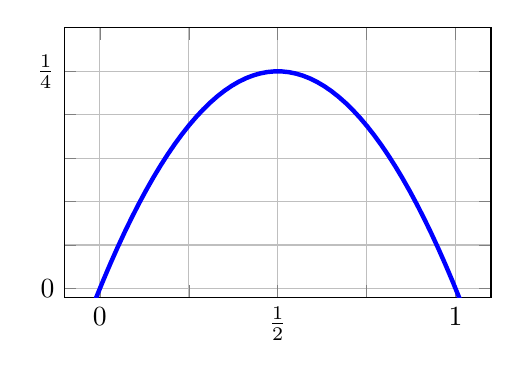
\begin{tikzpicture}
        \begin{axis}[width=7cm, height=5cm,xmin=-0.1,xmax=1.1,ymin=-0.01,ymax=0.3, xmajorgrids=true, ymajorgrids=true, xtick={0,0.25,0.5,0.75,1},  xticklabels={0,,$\frac{1}{2}$,,1}, ytick={0,0.05,0.1,0.15,0.2,0.25}, yticklabels={0,,,,,$\frac{1}{4}$},samples =500]
        \addplot[blue, ultra thick] (x,x-x*x);
        \end{axis}
    \end{tikzpicture}
    \caption{Gráfico de $p(1-p)$, cuyo vértice (punto max) se encuentra en (1/2,1/4)}
\end{figure}\\
Supongamos que queremos un intervalo de confianza al $95\%$, con error $\pm\varepsilon$.
\[0.95 \,\overset{!}{=}\,\pb\left(p\in[\hat{p}-\varepsilon\,,\,\hat{p}+\varepsilon]\right)= \pb\left(|\hat{p}-p|\leq\varepsilon\right) = \pb\left(\frac{|\hat{p}-p|}{\sigma/\sqrt{n}} \leq \frac{\varepsilon\sqrt{n}}{\sigma}\right)\]
Nuevamente, ocupando \textbf{T.C.L.}:
\[0.95\approx \pb\left(|\mathcal{N}(0,1)|\leq \frac{\varepsilon\sqrt{n}}{\sigma}\right)\,\Rightarrow
\,\frac{\varepsilon\sqrt{n}}{\sigma}\approx\,1.96\]
\[\Rightarrow\,\,\sqrt{n}\approx\,\frac{1.96\sigma}{\varepsilon}\,\,\Rightarrow\,\,n\approx\,\frac{1.96^2\sigma^2}{\varepsilon^2}\leq\frac{4\cdot 1/4}{\varepsilon^2}=\frac{1}{\varepsilon^2}\]
Así, ganamos una relación entre la cantidad de muestra que necesitamos para controlar el error asociado a la estimación. Por ejemplo, si queremos un error no mayor a $\varepsilon = 0.01$, bastaría con tomar $n=10000$ observaciones para lograrlo con $95\%$ de confianza.
\end{ejemplo}

\subsection{Simulación de variables aleatorias}
En la actualidad, todos los lenguajes de programación modernos poseen generadores de números \textit{pseudoaleatorios}\footnote{La palabra marca una diferencia respecto al término $aleatorio$, pero no se dará enfoque a este concepto en este curso.}. Tales programas producen como salida, una secuencia perfectamente determinista (y, a veces, periódica), pero cuyas propiedades estadísticas se parecen lo suficiente a las de una secuencia de realizaciones independientes de una variable aleatoria $unif(0,1)$. El problema de crear un "buen generador" de números aleatorios es crear una fórmula de recurrencia que, en un tiempo razonable, produzca una secuencia de números que se parezca lo más posible a una secuencia de realizaciones independientes $unif(0,1)$ con el periodo lo más largo posible.\footnote{ver  \cite[cap. 1]{Pard}}\\ Con este recurso computacional en mente, el objetivo ahora es recrear otras variables aleatorias con distribuciones diferentes que sean de interés, a partir de realizaciones uniformes en el intervalo $(0,1)$.\\ \newline
\begin{enumerate}
    \item \textbf{Simulación de una variable aleatoria Bernoulli:} Sea $0<p<1$. Si $U$ es una variable aleatoria $unif(0,1)$. Entonces $X=\mathbbm{1}_{\{U \leq p\}}$ es una variable $Bernoulli$ de parámetro $p$.
    \item \textbf{Simulación de una variable aleatoria Binomial:} Sea $n\in\N$, $U_1,U_2,\cdots,U_n$ variables aleatorias $i.i.d.$ $unif(0,1)$, entonces:
    \[X=\mathbbm{1}_{\{U_1\leq p\}} + \mathbbm{1}_{\{U_2\leq p\}}+\cdots + \mathbbm{1}_{\{U_n \leq p\}}\]
    es una variable aleatoria binomial de parámetros $n$ y $p$, $B(n,p)$.
    \item \textbf{Simulación de una variable aleatoria Geométrica:}
    \[X = \inf\{k\geq 1;\,U_k\leq p\}\]
    Cuando $(U_n)_n$ son variables aleatorias $i.i.d.$ con distribución $unif(0,1)$, \\entonces $X\sim geom(p)$.
\end{enumerate}
Para proceder a una simulación más eficiente nos basaremos en el siguiente lema.

\begin{lem} Sea $X$ una vaiable aleatoria, y $F$ su función de distribución ($i.e.$ $F(x) = \pb(X\leq x)$). Para $0\leq t\leq 1$, definimos:
\[F^{-1}(t) = \inf\{x;\,F(x)>t\}\]
Entonces, si $U$ tiene ley $unif(0,1)$, $F^{-1}(U)$ tiene ley $\mathcal{L}(X)$.
\end{lem}

\textbf{Demostración: }Notemos que si $F$ es una función invertible, entonces su inversa coincide con $F^{-1}$, además tendremos que $F^{-1}$ será una función creciente, al igual que $F$. Entonces:
\[\pb(F^{-1}(U)\leq t) = \pb(U\leq F(t)) = \int_{0}^{F(t)}dx = F(t) = \pb(X\leq t)\]
Donde la integral sale del hecho de que $U$ es una variable uniforme entre $[0,1]$ y $F(t)$ siempre pertenece a tal intervalo por ser una probabilidad.\\ \newline
¿Qué pasa cuando la función $F$ no es invertible? Notemos que $\forall\,x\in\R$:
\begin{equation}
    \{t\,:\,F^{-1}(t)\leq x\}\,\cup\,\{F(x)\}\,=\,\{t\,:\,t\leq F(x)\}
    \label{eq.dem1MC}
\end{equation}
En efecto: claramente $F(x)\in\,\{t\,:\,t\leq F(x)\}$, además:
\[F^{-1}(t)\leq x\,\Longleftrightarrow\,\inf\{y\,:\,F(y)>t\}\leq x\,\Longleftrightarrow\,\exists y*\leq x,\,\exists y_n\searrow y*,\,t.q.\,F(y_n)>t\,\forall\,n\]
Dado que $F$ es una función de distribución, es contínua por la derecha, entonces $F(y*)\geq t$. Ocupando que $F$ es creciente, tenemos:
\[y*\leq x\,\wedge\,F(y*)\geq t\,\Rightarrow\,F(x)\geq F(y*)\geq t\]
Esto prueba la inclusión $\subseteq$ en \ref{eq.dem1MC}. Recíprocamente, si $F(x)\geq t$ hay dos casos posibles:
\begin{itemize}
    \item Si $t=F(x)$, entonces el lado izquierdo de \ref{eq.dem1MC} corresponde al síngleton.
    \item Si $t<F(x)$, por definición de ínfimo:
    \[x\geq \inf\{y\,:\,F(y)>t\} = F^{-1}(t)\]
    Por lo tanto $t$ pertenece al lado izquierdo de \ref{eq.dem1MC} y se concluye la segunda inclusión.
\end{itemize}
Entonces, usando \ref{eq.dem1MC}; sea $Y=F^{-1}(U)$:
\[\pb(Y\leq y) = \pb(F^{-1}(U)\leq y)\]
Como $U$ es una variable aleatoria absolutamente contínua los síngleton tienen medida de probabilidad igual a cero. Así:
\[\pb(F^{-1}(U)\leq y) = \pb(F^{-1}(U)\leq y\,\vee\,U=F(y))\, \overset{\ref{eq.dem1MC}}{=}\,\pb(U\leq F(y)) = F(y)\]
Luego la función de probabilidad acumulada de $Y$ es $F$, es decir $Y\sim \mathcal{L}(X)$. \rule{0.7em}{0.7em}\\ \newline
En los casos en que la función de distribución $F$ tiene inversa de forma explícita, el lema anterior nos permita, cómodamente, simular realizaciones de la variable $X$.

\begin{ejemplo}[variable aleatoria exponencial.] Para $X\sim exp(\lambda)$, $F(x)=1-e^{-\labda x}$ $\forall\,x\geq 0$, luego:
\[F^{-1}(t) = -\frac{log(1-t)}{\lambda}\]
Por el lema anterior; para $U\sim unif(0,1)$.
\[F^{-1}(U) = -\frac{log(1-U)}{\lambda}\,\sim\,exp(\lambda)\]
Finalmente, si $U\sim unif(0,1)$ entonces la variable aleatoria $1-U$ también es uniforme en el intervalo [0,1], por lo tanto:
\[F^{-1}(U)\,\overset{d}{=}\,-\frac{log(U)}{\lambda}\,\sim\,exp(\lambda)\]
\end{ejemplo}

Una de las variables más importantes de simular son las variables aleatorias normales. Lamentablemente, el lema anterior no nos es de utilidad pues no conocemos una forma explícita de la función de distribución, sin embargo podemos hacer lo siguiente.\\ Si $U,V\,\sim unif(0,1)$ independientes, entonces:
\[X:= \sqrt{-2log(U)}cos(2\pi V)\hspace{0.3cm},\hspace{0.3cm}Y:=\sqrt{-2log(U)}sin(s\pi V)\]
son variables aleatoria con distribución $\mathcal{N}(0,1)$ independientes (\textbf{ejercicio, cambio de variable}). Luego, para generar $\mathcal{N}(\mu,\sigma^2)$, basta ponderar y trasladar de la forma $\sigma X + \mu$.\footnote{Los software ocupan algoritmos de mayor eficiencia para generar variables aleatorias normales, por ejemplo el algoritmo de Ziggurat.}

\subsection{Método de Aceptación-Rechazo}
Supongamos que conocemos $X$, una variable aleatoria con función de densidad $f$ conocida, pero sin $F^{-1}$ explícita. El objetivo es poder simular realizaciones de $X$, ¿cómo podemos simular $X$?\\ Supongamos que existe $Y$, una variable aleatoria eficientemente simulable, con función de densidad $g$ que cumpla lo siguiente:
\[\exists\,k>0,\hspace{0.5cm}f(x)\leq kg(x)\,\,\forall\,x\]
\[g(x)>0\,\Longleftrightarrow\,f(x)>0\]
Entonces, $\forall\,x$ tal que $g(x)>0$, definimos:
\begin{equation}
    \alpha(x) = \frac{f(x)}{kg(x)}
    \label{eq.alpha de x}
\end{equation}

\begin{prop} Sean $(Y_n,U_n)_n$ una secuencia de realizaciones independientes, tal que $U_n\sim unif(0,1)$, $Y_n\,\overset{d}{=}\,Y$ y $U_n$ es independiente de $Y_n$ para todo $n$. Definimos la variable aleatoria $N$ como:
\[N=\inf\{k\in\N\,:\,U_k \leq \alpha(Y_k)\}\]
Entonces $N<\infty$ c.s. y $Y_N \,\overset{d}{=}\,X$.
\end{prop}

\textbf{Demostración: }Veamos que $N<\infty$ $\pb-c.s.$ Para ello, notemos que:
\[\pb(N=\infty) = \pb(\forall\,m\,,\,U_m>\alpha(Y_m)) = \lim_{n \to \infty}\pb(\forall\,m=1,\cdots,n\,:\,U_m>\alpha(Y_m))\]
Como las realizaciones son $i.i.d.$ tenemos que:
\[\lim_{n \to \infty}\pb(\forall\,m=1,\cdots,n\,:\,U_m>\alpha(Y_m)) = \lim_{n \to \infty}\left[\pb(U_m > \alpha(Y_m))\right]^{n} = 0\]
Donde la última igualdad sale de que $\pb(U>\alpha(Y)) < 1$ (con la desigualdad estricta.\\ \newline
En efecto, sea $p=\pb(U\leq \alpha(Y))$, usando probabilidades totales:
\[p = \pb(U\leq \alpha(Y)) = \int_{\R}\pb(U\leq \alpha(y))g(y)dy= \int_{\R}\left(\int_{0}^{\alpha(y)}dx\right)g(y)dy\]
\[=\int_{\R}\alpha(y)g(y)dy = \int_{\R}\frac{f(y)}{kg(y)}g(y)dy = \frac{1}{k}\int_{\R}f(y)dy = \frac{1}{k}\,>\,0\]
Como $p>0$,entonces $1-p = \pb(U>\alpha(Y))<1$ y concluímos que $N<\infty$ $\pb-c.s.$\\ \newline
Ahora veamos que $Y_N \,\overset{d}{=}\,X$. $\forall\,A\subseteq \mathcal{B}(\R)$ tenemos que:
\[\pb(Y_N \in A) = \sum_{n=1}^{\infty}\pb(Y_n \in A,\,N=n) = \sum_{n=1}^{\infty}\pb(Y_n \in A,\,U_n\leq\alpha(Y_n),\,U_m>\alpha(Y_m),\,\forall\,m=1,\cdots,n-1)\]
\[=\sum_{n=1}^{\infty}(1-p)^{n-1}\pb(Y_n \in A,\,U_n\leq \alpha(Y_n))\]\[= \sum_{n=1}^{\infty}(1-p)^{n-1} \int_{\R}\pb(y \in A,\,U_n\leq \alpha(y))g(y)dy\]
Recordando que $U_n$ es uniforme, y (por lo visto al principio de la demostración) $p=1/k$:
\[\pb(Y_N \in A)= \sum_{n=1}^{\infty}(1-p)^{n-1} \int_{\R}\pb(y \in A,\,U_n\leq \alpha(y))g(y)dy\]\[= \sum_{n=1}^{\infty}(1-p)^{n-1}\int_{\R}\mathbbm{1}_{y\in A}\alpha(y)g(y) dy\]
\[=\sum_{n=1}^{\infty}(1-p)^{n-1}\int_{\R}\mathbbm{1}_{y\in A}\frac{f(y)}{kg(y)}g(y) dy\] \[= \sum_{n=1}^{\infty}(1-p)^{n-1}p\int_{\R}\mathbbm{1}_{y\in A}f(y) dy\] \[= \pb(X \in A)\sum_{n=1}^{\infty}p(1-p)^{n-1}= \pb(X\in A)\] 
\rule{0.7em}{0.7em}\\

Entonces, definiendo $\alpha(x) = \frac{f(x)}{kg(x)}$ para todo $x$ tal que $g(x)>0$. Explicamos el método de Aceptación-Rechazo mediante el siguiente algoritmo:\\ \newline
\textbf{Algoritmo Aceptación-Rechazo:} para simular la variable $X$.
\begin{enumerate}
    \item Simular $U\sim unif(0,1)$, simular $Y\sim g$. Ambas ($U$ e $Y$) independientes entre si.
    \item Si $U\leq \alpha(Y)$, $X=Y$ es un muestreo de $X$.
    \item Si $U> \alpha(Y)$, volver al paso 1 e iterar.
\end{enumerate}
\newline
\textbf{Observación: }De la demostración previa notamos que; $N\sim geom(1/k)$. Entonces el valor esperado de la cantidad de iteraciones necesarias para simular un valor de $X$ es $\E(N) = k$. Luego, para que el método termine en un tiempo razonable, es necesario ajustar el valor $k$ lo más cercano a 1 posible, es decir; elegir una densidad $g$ suficientemente parecida a $f$.\\ \newline
\textbf{Observación: }El método anterior es válido, aún tomando densidades con respecto a una medida $\mu$ cualquiera. Es decir, para $f$ y $g$ densidades de $X$ e $Y$, respectivamente, que cumplen las condiciones:
\[\prob\left(X\in A\right) = \int_{A}f(x)\mu(dx) \leq \int_{A}kg(x)\mu(x) = k\prob\left(Y\in A\right)\]
En particular, si $X$ es una variable aleatoria discreta, digamos en $\N$, entónces $f(x) = \prob(X=x)$ es la densidad de $X$ con respecto a la medida \textit{cuenta-puntos}. Luego, si $Y$ es otra variable aleatoria discreta que cumple las hipótesis con su densidad, es posible aplicar el método.

\subsection{Reducción de varianza}
Recordemos que el método de Monte Carlo (M.M.C.) aproxima un valor
\begin{equation}
    \alpha = \E(X) \approx \frac{1}{n}\sum_{i=1}^{n}X_i
    \label{redvar_1}
\end{equation}
donde $X_1,\cdots,X_n$ son copias $i.i.d.$ de $X$. Además sabíamos que el error es del orden de
$\frac{\sigma}{\sqrt{n}}$, con $\sigma^2 = Var(X)$.\\
Notamos que el valor por estimar en $\ref{redvar_1}$ sólo depende de la esperanza de la variable $X$ y no en la variable en sí o su distribución, por lo tanto tenemos la libertad de cambiar la variable a utilizar por una que tenga menor varianza, así estimaremos el mismo valor con un error menor.

\subsubsection{Muestreo preferencial}
Sea $X$ con densidad $f$. Sea el valor a estimar
\[\alpha = \E(g(X))\]
donde $g:\R\rightarrow\R$ es una función dada.\\ \newline
Ahora, supongamos que tenemos $Y$, otra variable aleatoria con densidad $\Tilde{f}>0$, entonces:
\[\alpha = \E(g(X)) = \int g(x)f(x) dx = \int \frac{g(x)f(x)}{\Tilde{f}(x)}\Tilde{f}(x) dx \]
Si definimos la función $h$ como:
\[h(x) = \frac{g(x)f(x)}{\Tilde{f}(x)}\]
Entonces $\alpha$ es la esperanza de la función $h$ bajo la densidad $\Tilde{f}$, es decir $\alpha = \E(h(Y))$. Además:
\[Var(h(Y)) = \E\left(h(Y)^2\right) - \alpha^2\]
\[= \int \frac{g(x)^2f(x)^2}{\Tilde{f}(x)^2}\Tilde{f}(x)dx - \alpha^2\]
\[= \int \frac{f(x)^2g(x)^2}{\Tilde{f}(x)}dx - \alpha^2\]
Si $g\geq 0$, entonces si escogemos \begin{equation}
    \Tilde{f}(x) = \frac{g(x)f(x)}{\alpha}
    \label{eq.rv2}
\end{equation}
entonces, obtenemos $Var(h(Y)) = 0$.\\ Evidentemente, \ref{eq.rv2} no funciona en la práctica, pues no conocemos el valor de $\alpha$. Sin embargo, nos sugiere que sería óptimo tomar una función $\Tilde{f}$ suficientemente parecido, en cuanto a forma, a $g(x)f(x)$ (diferenciado por una pondderación constante).\\ \newline

Esto motiva el siguiente procedimiento heurístico, escogeremos $\Tilde{f}$ cumpliendo:
\begin{itemize}
    \item $\Tilde{f}(x)$ "parecido" a $|g(x)f(x)|$, normalizado para que integre 1.
    \item Sea fácil de simular una variable $Y$, con densidad $\Tilde{f}$.
\end{itemize}
Luego basta aproximar $\alpha \approx \frac{1}{n}\sum_{i=1}^n h(Y_i)$, con $Y_1,\cdots,Y_n$ copias $i.i.d.$ de $Y$.\\ \newline

\textbf{Ejemplo: }Queremos aproximar:
\[I = \int_{0}^1 cos\left(\frac{\pi x}{2}\right)dx = \frac{2}{\pi}\]
Suponiendo que no podemos calcular esta integral, difiniendo:
\[I = \E(g(X)),\hspace{1cm}g(x) = cos\left(\frac{\pi x}{2}\right)\]
con $X$ una variable aleatoria uniforme en el intervalo $[0,1]$, podemos calcular $I$ mediante $M.M.C.$.\\ \newline
En este caso, podríamos reemplazar la función $coseno$ por un polinomio de grado 2. Dado que el interior de la integral es 0 en $x=1$ y 1 en $x=0$, es natural elegir $\Tilde{f}(x)$ de la forma $\lambda(1-x^2)$. Si normalizamos la función en este intervalo, tenemos que $\Tilde{f}(x) = 3(1-x^2)/2$. Al calcular las varianzas, podemos notar que el método reduce la varianza en un factor de 100. \\

\begin{figure}[h!]
    \centering
    \begin{tikzpicture}
        \begin{axis}[width=7cm, height=5cm,xmin=-0.1,xmax=1.1,ymin=-0.01,ymax=1.7, xmajorgrids=true, ymajorgrids=true, xtick={0,0.25,0.5,0.75,1},  xticklabels={0,,,,1}, ytick={0,0.25,0.5,0.75,1,1.25,1.5}, yticklabels={0,,,,1,,1.5},samples =500]
        \addplot[blue, ultra thick] (x,1.5-1.5*x*x);
        \addplot[red, ultra thick](x,cos(deg(1.5707*x)));
        \end{axis}
    \end{tikzpicture}
    \caption{En rojo la función $cos(\pi x/2)$, en azul la función $3(1-x^2)/2$ mayorándola.}
\end{figure}\\

\subsubsection{Variable de control}
Este método involucra escribir $\E(f(X))$ de la forma:
\[\E\left(f(X)\right) = \E\left(f(X)-h(X)\right) + \E\left(h(X)\right)\]
Donde $\E\left(h(X)\right)$ puede ser calculado explícitamente, y $Var\left(f(X)-h(X)\right)$ es significatívamente menor que $Var\left(f(X)\right)$. Así, empleamos el método de Monte Carlo para el cálculo de $\E\left(f(X)-h(X)\right)$ y el cálculo directo de $\E\left(h(X)\right)$.\\ \newline
\textbf{Ejemplo: }Sumpogamos que deseamos calcular la siguiente integral:
\[I = \int_{0}^1 e^x dx = e-1\]
Aplicando el $M.M.C.$, con $I=\E(e^X) = \E(g(X))$, con $X\sim unif(0,1)$. Notamos que la varianza de la función es $Var(g(X)) \approx 0,242$.\\
Dado que, cerca de $x=0$, $e^x \approx 1+x$, podemos escribir:
\[\int_{0}^1 e^x dx = \int_{0}^1 (e^x -1-x)dx + \frac{3}{2}\]
En este caso, elegimos $h(x)=1+x$. Es fácil comprobar que $Var\left(g(x)-h(x)\right) \approx 0.0437$. Es decir, hemos reducido la varianza de la estimación en un factor de $5.5$ aproximadamente.

\subsubsection{Variables antitéticas}
Supongamos que deseamos calcular la siguiente integral;
\[I =   \int_{0}^1 f(x)dx\]
Dado que el cambio de variable: $x\rightarrow 1-x$ es invariante ante la medida $dx$ en $[0,1]$. Es decir,
\[\int_{0}^1f(x)dx = \int_{0}^1f(1-x)dx\]
Entonces es posible reescribir $I$ de la sigueinte forma:
\[I = \frac{1}{2}\int_{0}^1 (f(x) + f(1-x))dx\]
Otra forma de plantear el problema, es definir la variable aleatoria $X\sim unif(0,1)$. Así, $1-X \sim unif(0,1)$, entonces:
\[I = \E(f(X)) = \E\left(\frac{f(X)+f(1-X)}{2}\right)\]
y obtenemos la misma conclusión.\\ \newline

Ahora, podemos calcular $I$ con $M.M.C.$. Simulamos $n$ variables aleatorias $i.i.d.$ uniformes en $[0,1]$, $U_1,\cdots,U_n$, y aproximamos $I$ por:
\[I_{2n} = \frac{1}{n}\left(\frac{1}{2}(f(U_1)+f(1-U_1))+ \cdots + (f(U_n)+f(1-U_n))\right)\]
\[= \frac{1}{2n}(f(U_1)+f(1-U_1) + \cdots + f(U_n) + f(1-U_n))\]
A grandes razgos, este método es equivalente a emplear el método tradicional de Monte Carlo, con la variable $\frac{f(U)+f(1-U)}{2}$. Podemos observar que su varianza:
\[Var\left(\frac{f(U)+f(1-U)}{2}\right) = \frac{1}{4}Var\left(f(U) + f(1-U)\right)\]
\[= \frac{1}{4}\left(Var\left(f(U)\right) + 2Cov\left(f(U),f(1-U)\right) + Var\left(f(1-U)\right)\right)\]
Dado que $X\overset{d}{=}1-X$:
\[Var\left(\frac{f(U)+f(1-U)}{2}\right) = \frac{1}{2}\left[Var(f(U)) + Cov(f(U),f(1-U))\right]\]
Así, si $Cov(f(U),f(1-U)) \leq 0$, se reduce la varianza de la estimación en al menos un factor de 1/2.\\ \newline
En general, tenemos que la aproximación mejora siempre que:
\[\E\left(f(U)f(U-1)\right) < \E\left(f(U)^2\right)\]

\begin{lem} Si $f$ es una función \textit{monótona}, entonces:
\[Cov(f(U),f(1-U)) \leq0\]
\end{lem}
\subsubsection{Método de Estratificación}
Este método es bien conocido en el diseño de muestras de encuestas. Supongamos que se busca calcular
\[I = \E\left(g(X)\right) = \int g(x)f(x)dx\]
Donde $X$ tiene ley $f(x)dx$. Consideremos $D_1,\cdots,D_m$, una partición del soporte de la densidad $f$. Luego, podemos descomponer $I$ en
\begin{equation}
    I = \sum_{i=1}^m I_i = \sum_{i=1}^m \E\left(\mathbbm{1}_{\{X\in D_i\}}g(X)\right)
    \label{eq_estrat1}
\end{equation}

Este método propone estimar $I_i$ con $M.M.C.$, usando $n_i$ simulaciones. Definimos como $\sigma_i^2 = Var(\mathbbm{1}_{\{X\in D_i\}}g(X))$. Entonces, la varianza de la aproximación es

\begin{equation}
    \sum_{i=1}^m \frac{\sigma_i^2}{n_i}
    \label{eq_estrat2}
\end{equation}

Si minimizamos \ref{eq_estrat2}, bajo la restricción de un número de simulaciones $\sum_{i=1}^m n_i = n$ dado, obtenemos $n_i =n\sigma_i/\sum_{i=1}^m\sigma_i$, con un valor mínimo de la varianza de
\[\frac{\left(\sum_{i=1}^m \sigma_i\right)^2}{n}\]
Puede probarse que esta varianza es menor que la obtenida con $n$ simulaciones bajo el método estándar de Monte Carlo directamente en \ref{eq_estrat1}. Por supuesto, rara vez es posible calcular el valor de $\sigma_i$, lo que limita el uso de esta técnica (pero bien uno puede estimarlos vía su estimador insesgado de varianza mínima $\frac{1}{n-1}\sum (x_i-\Bar{x})^2$, o bajo el propio $M.M.C.$).

\section{Cadenas de Markov}
Una cadena de Markov es una sucesión de variables aleatorias $\left\{X_n;n=0,1,2,...\right\}$, definidas sobre algún espacio de probabilidad $\left(\Omega,\mathcal{
F}, \prob\right)$, tomando valores en un conjunto $E$ arbitrario, pero que supondremos que será finito o numerable, y que posee la propedad de Markov. Intuitívamente, una cadena de Markov posee la cualidad de que, conociendo el estado presente $X_n$, sin necesidad de conocer los estados anteriores puede hacer buenas predicciones acerca de los estados futuros.\\ Los siguientes temas presentan variadas aplicaciones de las cadenas de Markov. Tenga en cuenta que restringiremos el contenido a cadenas de Markov \textit{homogéneas}, aunque el caso no homogéneo sea necesario en muchas aplicaciones.

\subsection{Definiciones y propiedades elementales}

\begin{definicion}
Sea $E$ un conjunto finito o numerable. Un proceso estocástico $\{X_n;n\in \N\}$ es llamado \textit{Cadena de Markov} si, para todo $n\in\N$, la ley condicional de $X_{n+1}$ dado $X_0,X_1,\cdots,X_n$, es igual a la ley condicional de $X_{n+1}$ dado $X_n$.\\ \newline Esto es; $\forall\,x_0,\cdots,x_n\,\in E$:
\[\prob\left(X_{n+1}=x_{n+1}\,|\,X_o = x_0,\,X_1=x_1,\,\cdots,\,X_n=x_n\right) = \prob\left(X_{n+1}=x_{n+1}\,|\,X_n=x_n\right)\]
La cadena se dirá 'Homogénea', si lo anterior no depende del índice $n$. En cuyo caso, la matriz $P=\left(P_{xy}\right)_{x,y\in E}$, con $P_{x,y} = \prob\left(X_{n+1}=y\,|\,X_n = x\right)$\\ \newline
Además, llamamos $\mu\in \mathcal{P}(E)$ a $\mu_x = \prob(X_0 = x)$, denominada 'Distribución inicial'. Así, decimos que $\left(X_n\right)_{n\in\N}$ es una $(\mu,P)$-cadena de Markov homogénea.
\end{definicion}

\begin{ejemplo}
En $E=\Z$, si $Z_0,Z_1,Z_2,...$ son las ganancias de apuestas modeladas como variables aleatorias $i.i.d.$, entonces la ganancia total acumulada $X_n = \sum_{i=0}^nZ_i$ es una cadena de arkov ($C.M.$).
\end{ejemplo}

Un simple criterio, que nos permitirá en muchos casos verificar si un proceso dado es C.M., está dado por el siguiente lema.

\begin{lem}
Sean $E$ y $F$ dos conjuntos numerables, y sea $f$ un mapeo de $\N\times E \times F$ hacia $E$. Sean $X_0,Y_1,Y_2,...$, son variables aleatorias mútuamente independientes, siendo $X_0$ valor en $E$ e $Y_n$ valores en $F$.\\ 
Sean $\{X_n;\,n\geq 1\}$ un proceso en $E$, definido como:
\[X_{n+1} = f(n,X_n,Y_{n+1}),\hspace{0.7cm}n\in\N\]
Entonces $\{X_n;\,n\in\N\}$ es cadena de Markov.
\end{lem}

\textbf{Demostración: }
\[\prob\left(X_{n+1} = x_{n+1}\,|\,X_0=x_0,\,\cdots,\,X_n=x_n\right) = \frac{\prob\left(X_0=x_0,\,\cdots,\,X_n=x_n,\,X_{n+1}=x_{n+1}\right)}{\prob\left(X_0=x_0,\,\cdots,\,X_n=x_n\right)}\]
\[ = \sum_{\{z;f(n,x_n,z)=x_{n+1}\}}\frac{\prob\left(X_0=x_0,\,\cdots,\,X_n=x_n,\,Y_{n+1}=z\right)}{\prob\left(X_0=x_0,\,\cdots,\,X_n=x_n\right)}\]
Dado que $Y_{n+1}$ es una variable independiente a todos los valores $\{X_0,\cdots,X_n\}$, entonces:
\[ = \sum_{\{z;f(n,x_n,z)=x_{n+1}\}}\frac{\prob\left(X_0=x_0,\,\cdots,\,X_n=x_n,\,Y_{n+1}=z\right)}{\prob\left(X_0=x_0,\,\cdots,\,X_n=x_n\right)}\]
\[ = \sum_{\{z;f(n,x_n,z)=x_{n+1}\}}\frac{\prob\left(X_0=x_0,\,\cdots,\,X_n=x_n\right)\prob\left(Y_{n+1}=z\right)}{\prob\left(X_0=x_0,\,\cdots,\,X_n=x_n\right)}\]
\[ = \sum_{\{z;f(n,x_n,z)=x_{n+1}\}}\prob\left(Y_{n+1}=z\right)\]
\[=\frac{\prob\left(X_n = x_n,\,X_{n+1}=x_{n+1}\right)}{\prob\left(X_n =x_n\right)} = \prob\left(X_{n+1}=x_{n+1}\,|\,X_n=x_n\right)\]
\rule{0.7em}{0.7em}\\ \newline

Una cadena de Markov es el análogo de una sucesión determinista determinada por una relación de recurrencia del tipo
\[x_{n+1} = f(n,x_n),\]
opuesto al sistema 'con memoria', del tipo
\[x_{n+1} = f(n,x_n,x_{n-1},\cdots,x_0).\]
Acá la función $f(n,\cdot)$ es reemplazada por la matriz de trancisión
\[P_{xy}= \prob\left(X_{n+1}=y\,|\,X_n =x\right).\]
Hasta el momento, podemos asumir que la matriz $P=\left(P_{xy}:\,x,y\in E\right)$ es independiente de la variable tiempo $n$, una vez dicho que la cadena es \textit{homogénea}.

\begin{lem}
\label{Lema 8}
Sea $f:E\times [0,1]\rightarrow E$ medible, sea $X_0$ variable aleatoria en $E$, $Y_1,Y_2,\cdots,$ variables aleatorias uniformes en $[0,1]$, todas independientes entre sí (y de $X_0$). Entonces $\left(X_n\right)_{n\in\N}$ definido recursivamente por $X_{n+1} = f(X_n,Y_{n+1})$ es una $C.M.H.$ (cadena de Markov homogénea).
\end{lem}
 La matriz $P$ es llamada \textit{Markoviana} (o \textit{estocástica}), en el sentido en que tiene la siguiente propiedad; para cada $x\in E$, el vector fila $\left(P_{xy};\,y\in E\right)$ es una medida de probabilidad en $E$, en otras palabras;
 \[P_{xy}\geq 0,\hspace{0.2cm}\forall\,y\in E;\hspace{0.5cm}\sum_{y\in E}P_{xy} = 1\]
 El vector de distribución inicial, definido por $\mu_x = \prob\left(X_0 = x\right)$, se entiende como un vector fila, de modo que $\left(\mu P\right)_y = \sum_{x\in E}\mu_xP_{xy}$.\\ \newline
 
\begin{prop}
Para una $(\mu,P)$-$C.M.H.$ se cumplen:
\begin{enumerate}
    \item[i)] $\prob\left(X_0=x_0,\,\cdots,\,X_n=x_n\right) = \mu_{x_0}P_{x_0x_1}P_{x_1x_2}\cdots P_{x_{n-1}x_n}$.(Esta propiedad es equivalente a la definición de $(\mu,P)-C.M.H.$)
    \item[ii)] $\prob\left(X_{n+1}=x_{n+1},\,\cdots,\,X_{n+m}=x_{n+m}\,|\,X_0=x_0,\cdots,X_n=x_n\right) = P_{x_{n+1}x_{n+2}}\cdots P_{x_{n+m-1}x_{n+m}}$.
    \item[iii)] $\prob\left(X_n=y\,|\,X_0=x\right) = \left(P^n\right)_{xy}$ (Donde la notación anterior hace referencia a la potencia matricial).
    \item[iv)] $\prob\left(X_n = y\right) = \left(\mu P^n \right)_{y}$
    \item[v)] Para $g:E\rightarrow \R$, 
    \[\E\left(g(X_n)\,|\,X_0 = x\right) = \left(P^ng\right)_x = \sum_{y\in E} P^n_{xy} g(y)\]
    \item[vi)] $\E\left(g(X_n)\right) = \mu P^n g = \sum_{x,y\in E}\mu_x P^n_{xy}g_y$
\end{enumerate}
(En esta proposición hacemos uso de la notación $g_y = g(y)$).
\end{prop}

\textbf{Demostración: }\cite[págs. 20,21]{Pard}\\ \newline

\subsection{Propiedad de Markov fuerte}
Para la mejor comprensión de esta parte, recordemos la propiedad de Markov. Sea $\left\{X_n;n\in \N\right\}$ una cadena de Markov a valores en $E$ definida sobre el espacio de probabilidades $\left(\Omega,\mathcal{F},\prob\right)$. Dada una medida de probabilidad $\mu$ sobre $E$, usaremos la notación $\prob_{\mu}$ para denotar cualquier probabilidad sobre $\left(\Omega,\mathcal{F}\right)$ tal que, bajo $\prob_{\mu}$, la sucesión $\{X_n; n\geq 0\}$ es una cadena de Markov con ley inicial $\mu$; en otras palabras, $\mu$ es la ley de $X_0$, esto es,
\[\prob_{\mu}\left(X_0=x\right) = \mu_x, \hspace{0.5cm}x\in E.\]
parael caso $\mu = \delta_x$, escribiremos $\prob_x$ en vez de $\prob_{\delta_x}$.\\ $\prob_x$ puede ser interpretado como la ley condicional de $X$, dado $X_0=x$. Para cualquier $n\geq 0$, definimos $\mathcal{F}_n$ como la sigma-algebra de los eventos que están determinados por las variables $X_0,X_1,\cdots,X_n$, esto es,
\[\mathcal{F}_n = \left\{\{\omega; \left(X_0(\omega),\cdots,X_n(\omega)\right)\in B_n\};\,B_n \in 2^{E^{n+1}}\right\}\]
Donde $2^F$ denota la colección de todos los subconjuntos del conjunto $F$.

\begin{teorema}
Sea $\{X_n; n\geq 0\}$ una $(\mu,P)$ cadena de Markov. Entonces, para cada $n\in \N,$ $x\in E$, condicionalmente a $\{X_n=x\}$, $\{X_{n+p}; p\geq 0\}$ es una $(\delta_x,P)$-cadena de Markov independiente  de $\left(X_0,X_1,\cdots,X_n\right)$. En otras palabras, para todo $A \in \mathcal{F}_n$ y todo $m>0$, $x_1,\cdots,x_m \in E$,
\[\prob\left(A\cap\{X_{n+1}=x_1,\cdots,X_{n+m} = x_m\}|X_n=x\right)\]
\[= \prob\left(A|X_n=x\right)\prob_x\left(X_1 = x_1,\cdots,X_m = x_m\right)\]
\end{teorema}
\textbf{Demostración: }Es suficiente probar el resultado en el caso donde $A=\{X_0=y_0,X_1=y_1\cdots,X_n=y_n\}$ ($A$ es unión finita o numerable de conjuntos disjuntos de esta forma, y el resultado en el caso general saldrá de la $\sigma$-aditividad de $\prob$). Es suficiente considerar el caso $y_n =x$. Así, el lado izquiero de la igualdad es equivalente a
\[\frac{\prob\left(X_0=y_0,\cdots,X_n=x,X_{n+1}=x_1,\cdots,X_{n+m}=x_m\right)}{\prob\left(X_n=x\right)},\]
así, aplicando la propiedad anterior iterativamente, esto es igual a
\[\frac{\prob(A)}{\prob\left(X_n=x\right)}\times P_{xx_1}\times P_{x_1x_2}\times \cdots \times P_{x_{m-1}x_m},\]
o, en otras palabras,
\[\prob\left(A|X_n=x\right)\prob_x\left(X_1=x_1,\cdots,X_m=x_m\right).\]
\rule{0.7em}{0.7em}\\ \newline

El último resultado nos dice en particular que, el pasado y el futuro de una cadena son condicionalemnte independientes, dada la posición de la cadena en el tiempo presente $n$.\\ Ahora, nos gustaría expandir la propiedad de Markov, reemplazando el tiempo dado $n$ por un tiempo aleatorio (pero no cualquier tiempo aleatorio).

\begin{definicion}
Una variable aleatoria $T$ que toma valores en el conjunto $\N\cup \{+\infty\}$ es llamada tiempo de parada (t.d.p.) si, para todo $n\in \N$,
\[\{T=n\} \in \mathcal{F}_n.\]
\end{definicion}
En otras palabras, las observaciones $X_1,X_2,\cdots,X_n$, la trayectoria de la cadena en el tiempo $n$, es suficiente para decidir si $T$ es igual a $n$.

\begin{ejemplo}
    \begin{enumerate}
        \item Para cada $x\in E$, el tiempo de llegada al estado $x$,
        \[S_x = \begin{cases}
        \inf\{n\geq0;\,X_n=x\} & \text{, si existe $n$ que lo cumpla.}\\
        +\infty & \text{, otro caso.}
        \end{cases}\]
        y el tiempo del primer retorno al estado $x$,
        \[T_x = \begin{cases}
        \inf\ & \text{, si existe $n$ que lo cumpla.}\\
        +\infty & \text{, en otro caso.}
        \end{cases}\]
        son tiempo de parada\footnote{Con la convención de que el ínfimo de un conjunto vacío es $+\infty$, basta con escribir: $T_x = \inf\{n\geq 1;\,X_n=x\}$.}. En el caso de $T_x$ esto se cumple porque
        \[\{T_x = n\} = \{X_1\neq x\}\cap \cdots \cap \{X_{n-1}\neq x\}\cap\{X_n = x\}.\]
        \item $\forall\,A\subseteq E$, $T_A := \inf\{n\geq 0:\,X_n\in A\}$ es el tiempo de llegada al conjunto $A$. $T_A$ es t.d.p.
        \item $L_A:= \sup\{n\geq 1:\,X_n\in A\}$ es la última vez que  la cadena visita $A$. No es tiempo de parada, puesto que necesitamos conocer la trayectoria luego del tiempo $n$ para decidir si $L_A = n$, o no.
    \end{enumerate}
\end{ejemplo}\\ \newline \newline
Dado un tiempo de parada $T$, anotamos
\[\mathcal{F}_T := \{B \in \mathcal{F}\,|\,B\cap \{T=n\} \in \mathcal{F}_n,\, \foralln\}\]
Donde $\left(\Omega,\mathcal{F},\prob\right)$ es el espacio de probabilidades subyaccente.\\ (\textbf{Propuesto: }$\mathcal{F}_T$ es una $\sigma$-álgebra)

\begin{teorema}[Propiedad de Markov-fuerte.]
Sea \{X_n;\,n\geq 0\} una $(\mu,P)$-C.M., y $T$ un tiempo de parada. Condicionado a $\{T<\infty\}\cap\{X_T = x\}$, $\{X_{T+n};\,n\geq 0\}$ es una $(\delta_x,P)$-C.M. que es independiente de $\mathcal{F}_T$.\\ \newline
En otras palabras; para todo $A\in \mathcal{F}_T$ y todo $m>0$, $x_1,\cdots,x_m \in E$,
\[\prob\left(A\cap\{X_{T+1}=x_1,\cdots,X_{T+m}=x_m\}\,|\,X_T=x,\,T<\infty\right)\]
\[= \prob\left(A\,|\,X_T = x,\,T<\infty\right)\times\prob_x\left(X_1 = x_1,\cdots,X_m = x_m\right).\]
\end{teorema}\\ \newline
\textbf{Demostración: }Es suficiente mostrar que, para todo $n\in \N$,
\[\prob\left(A\cap\{T=n\}\cap\{X_{T+1}=x_1,\cdots,X_{T+m}=x_m\}\,|\,X_T=x\right)\]
\[= \prob\left(A\cap\{T=n\}\,|\,X_T = x\right)\prob_x\left(X_1 = x_1,\cdots,X_m=x_m\right),\]
que es resultado directo de la propiedad markoviana.\\ \newline
\rule{0.7em}{0.7em}\\ \newline

\subsection{Estados Recurrentes y Transientes }
Definimos $T_x = \inf\{n\geq 1;\,X_n = x\}$ como en  el ejemplo anterior.\\ \newline

\begin{definicion}
$x\in E$ se dice \textit{recurrente} si $\prob_x\left(T_x <\infty\right)=1$, y \textit{transiente} en el caso contrario (es decir, si $\prob_x\left(T_x<\infty\right)<1$).
\end{definicion}
 Definimos además, el número de retornos al estado $x$:
 \[N_x = \sum_{n\geq 1}\mathbbm{1}_{\{X_n = x\}}.\]
 
 \begin{prop}
    \begin{enumerate}
        \item[a)] Si $x$ es recurrente, entonces
        \[\prob_x\left(N_x = +\infty\right) = 1.\]
        \item[b)] Si $x$ es transiente, entonces
        \[\prob_x\left(N_x =k\right) = \left(1 - p_x\right)p_x^k,\hspace{0.3cm}k\geq 0,\]
        donde $p_x = \prob_x\left(T_x<\infty\right)$ (en particular, $N_x<\infty$, $\prob_x$-c.s.).
    \end{enumerate}
 \end{prop}\\ \newline
\textbf{Demostración: }Sea 
\[T_x^2 = \inf\{n> T_x;\,X_n=x\}\]
\[= T_x + \inf\{n\geq 1;\,X_{T+n}=x\}.\]
No es difícil ver que $T_x^2$ es un tiempo de parada:
\[\prob_x\left(T_x^2 < \infty\right) = \prob_x\left(T_x^2<\infty\,|\,T_x<\infty\right)\prob_x\left(T_x<\infty\right)\]
\[= \sum_{n=1}^{\infty}\prob_x\left(T_x^2= T_x + n\,|\,T_x<\infty\right)\prob_x\left(T_x <\infty\right).\]
Pero, por la propiedad de Markov fuerte, deducimos que
\[\porb_x\left(T_x^2 = T_x +n\,|\,T_x<\infty\right)\]
\[=\prob_x\left(X_{T_x +1}\neq x,\cdots,X_{T_x +n-1}\neq x,X_{T_x +n}=x\,|\,T_x<\infty\right)\]
\[= \prob_x\left(X_1\neq x,\cdots,X_{n-1}\neq x,X_n=x\right)\]
\[=\prob_x\left(T_x=n\right).\]
Finalmente,
\[\prob_x\left(T_x^2<\infty\right)=(\prob_x\left(T_x<\infty\right))^2\]
o
\[\prob_x\left(N_x\geq 2\right) = (\prob_x\left(T_x<\infty\right))^2.\]
Así, iterando el mismo argumento, deducimos que
\
Ambas afirmaciones de la proposición se deducen fácilmente de esta identidad.\\
\rule{0.7em}{0.7em}\\ \newline
\begin{cor}
$x$ es recurrente si y sólo si
\[\sum_{n=0}^{\infty}\left(P^n\right)_{xx} = +\infty.\]
\end{cor}
\textbf{Demostración: }Notemos que
\[\E_x(N_x) = \E_x\left(\sum_{n\geq 1}\mathbbm{1}_{\{X_n=x\}}\right) = \sum_{n\geq 1}\prob_x\left(X_n=x\right)\]
\[= \sum_{n\geq 1}\left(P^n\right)_{xx}.\]
Si $x$ es recurrente, entonces $N_x=\infty$ $\prob_x$-c.s., luego $\E(N_x)=\infty$, probando ($\Longrightarrow$).\\ \newline
Recíprocamente, si $x$ es transiente, por la parte \textbf{b)} de la proposición anterior, se tiene que $\E_x(N_x)<\infty$, con lo cual se prueba ($\Longleftarrow$).\\
\rule{0.7em}{0.7em}\\ \newline

\begin{definicion}
Decimos que un estado $y$ es accesible desde el estado $x$ (y anotamos $x\rightarrow y$), siempre que exista $n\geq 0$ tal que $\prob_x\left(X_n=y\right)>0$. Decimos que $x$ e $y$ se comunican (y escribimos $x\leftrightarrow y$) cuando $y\rightarrow x$,  además de $x\rightarrow y$. 
\end{definicion}

La relación $x\leftrightarrow y$ es una relación de equivalencia, entonces podemos particionar el conjunto $E$ en clases de equivalencia definidas por la relación $\leftrightarrow$.\\
Notamos que $x\leftrightarrow y$ $\Longleftrightarrow$ $\exists\,n\geq 0$ tal que $\left(P^n\right)_{xy}>0$, dado que $\prob_x\left(X_n=y\right)=\left(P^n\right)_{xy}$.  \\ \newline

\begin{teorema}
Sea $C\subset E$ una clase de equivalencia de la relación $\leftrightarrow$. Entonces todos los estados de $C$ son recurrentes, o bien, son todos transientes.
\end{teorema}

\textbf{Demostración: }\cite[págs. 26- Teo.4.5]{Pard}\\ \newline
Luego, las clases de equivalencia definidas por $\leftrightarrow$, se les llaman clases de recurrencia.

\begin{definicion}
Una $(\mu,P)$-C.M. se dice irreducible cuando $E$ consiste sólo de una clase de equivalencia . Se dirá irreducible y recurrente si es reducible y además esa calse de equivalencia es  recurrente.
\end{definicion}

\begin{prop}
Toda cadena de Markov irreducible sobre un espacio de estados $E$ finito, es recurrente.
\end{prop}

\textbf{Demostración: }Dado que $E$ es finito, al menos un estado debe ser visitado infinitas veces con probabilidad positiva, por lo tanto,  casi seguramente, por la proposición anterior, este estado (y todos los de la calse) es (son) recurrente.\\
\rule{0.7em}{0.7em}\\ \newline

\subsection{Casos Irreducibles y Recurrentes}
En esta sección, asumiremos que una cadena es irreducible y recurrente. Empezaremos estudiando las \textit{excursiones} de una cadena entre dos retornos sucesivos al mismo estado $x$:
\[\varepsilon_k = (X_{T_x^k},X_{T_x^k+1},\cdots,X_{T_x^{k+1}}),\hspace{0.3cm}k\geq 0.\]
Tales excursiones son secuencias aleatorias de largo aleatorio, al menos 2 y finito, compuesta de elementos $E\textbackslash{}\{x\}$, excepto por el primero y el último, que son iguales a $x$. Denotamos como $U$ al conjunto de secuencias
\[u = (x,x_1,\cdots,x_n,x),\]
con $n\geq 0$, $x_l\neq x$, $1\leq l \leq n$. $U$ es numerable, y es el conjunto de todas las posibles excursiones $\varepsilon_0,\varepsilon_1,...$. Por lo tanto, estas variables aleatorias toman valores en un conjunto numerable, y sus leyes de probabilidad están caracterizadas por las cantidades
\[\prob\left(\varepsilon_k = u\right),\hspace{0.3cm}u\in U.\]

\begin{prop}
Bajo $\prob_x$, la secuencia $(\varepsilon_0,\varepsilon_1,\cdots)$ de excursiones es $i.i.d.$, en otras palabras, existen probabilidades $\{p_u;\,u\in U\}$ sobre $U$ tal que, para todo $k>0$, $u_0,u_1,\cdots,u_k\,\in U$,
\[\prob_x\left(\varepsilon_0 = u_0,\,\varepsilon_1 = u_1,\,\cdots,\,\varepsilon_k = u_k\right) = \prod_{l=0}^k p_{u_l}.\]
\end{prop}

\textbf{Demostración: }Esto es consecuencia de la propiedad fuerte de Markov. En efecto,\newline $\{\varepsilon_0 = u_0\}\in \mathcal{F}_{T_x}$, y el evento
\[\{\varepsilon_1 = u_1,\cdots,\varepsilon_k = u_k\}\]
es de la forma
\[\{X_{T_x+1}=x_1,\cdots,X_{T_x+p}=x_p\},\]
pára algún $p>0$, $x_1,\cdots,x_p\,\in E$. En consecuencia,
\[\prob_x\left(\varepsilon_0 = u_0,\varepsilon_1 = u_1,\cdots, \varepsilon_k = u_k\right)\]
\[= \prob_x\left(\{\varepsilon_0 = u_0\}\cap\{X_{T_x+1}=x_1,\cdots,X_{T_x +p}=x_p\}\,|\,T_x <\infty\right)\]
\[\prob_x\left(\varepsilon_0 =u_0\right)\prob_x\left(X_1=u_1,\cdots,X_p =x_p\right)\]
\[=\prob_x\left(\varepsilon_0=u_0\right)\prob_x\left(\varepsilon_0=u_1,\cdots,\varepsilon_{k-1}=u_k\right)\]
\[=\prob_x\left(\varepsilon_0 =u_0\right)\prob_x\left(\varepsilon_0=u_1\right)\cdots\prob_x\left(\varepsilon_{k-1}=u_k\right)\]
\[=p_{u_0}p_{u_1}\cdots p_{u_k},\]
donde $\{p_u;\,u\in U\}$ es la ley de $\varepsilon_0$ bajo $\prob_x$.\\
\rule{0.7em}{0.7em}\\ \newline
Una medida (no necesariamente de probabilidad) sobre el conjunto $E$, es un 'vector fila' $\{\gamma_x;\,x\in E\}$ tal que $0\leq \gamma_x < \infty$, para todo $x$. Cuando la medida es finita, $\sum_{x\in E}\gamma_x <\infty$, podemos normalizarla, haciéndola medida de probabilidad sobre $E$, $\left(\gamma_x / \sum_{z\in E}\gamma_z\, ;\,x\in E\right)$.\\ Una medida $\gamma$ se dice \textit{invariente} (respecto a la matriz de transición $P$) cuando
\[\gamma P = \gamma,\]
esto es, 
\[\sum_{y\in E}\gamma_y P_{yx} = \gamma_x,\hspace{0.3cm}\forall\,x\in E.\]
Una medida $\gamma$ se dice \textit{estríctamente posita} si $\gamma_x >0$, para todo $x\in E$.\\ \newline

Una medida $\gamma$ es invariante si y sólo si  la cadena $(\gamma,P)$ cumple $\mathcal{L}(X_n)=\gamma$, $\forall\,n\in \N$. Esto es, $\gamma$ es la ley de $X_n$ para todo valor de $n$.\\ Dado que es para todo $n$, $\{X_{n+m};\,m\in\N\}$ también es $(\gamma,P)$-C.M.\\ \newline
\textbf{Observación: }Una \textbf{probabilidad} invariante es una medida de probabilidad  $\pi$, que satisface $\pi P = \pi$, o equivalentemente, para todo $x\in E$,
\[\sum_{y\neq x}\pi_y P_{yx} = \pi_x\left(1- P_{xx}\right)\]
esto es,
\[\prob\left(X_n\neq x ,X_{n+1}=x\right) = \prob\left(X_n = x,X_{n+1}\neq x\right)\]
lo que significa que en el equilibrio, el número medio de salidas  desde el estado $x$ entre los tiempo $n$ y $n+1$ es igual al número medio de llegadas al estado $x$ entre los mismos tiempos. Esta es la intuición que caracteriza a la probabilidad invariante.

\begin{teorema}
Sea $\{X_n\,;\,n\in N\}$ una C.M. irreducible y recurrente. Entonces existe una medida invariante $\gamma$ estrictamente positiva, cual es única salvo constantes multiplicativas.
\end{teorema}

\textbf{Demostración: }Para probar la existencia, sea $\gamma_y^x$ el número esperado de visitas al estado $y$ durante la excursión $\varepsilon_0$ partiendo de $x$, esto es,
\[\gamma_y^x = \E_x\left(\sum_{n=1}^{T_x}\mathbbm{1}_{X_n=y}\right)\]
\[= \sum_{n=1}^{\infty}\prob_x \left(X_n = y,\, n\leq T_x\right)\]
\[=\sum_{z\in E}\sum_{n=1}^{\infty}\prob_x(\{X_{n-1}=z,\,n-1<T_x\}\cap\{X_n = y\})\]
\[=\sum_{z\in E}\left(\sum_{n=2}^{\infty}\prob_x(X_{n-1} = z,\,n-1\leq T_x)\right)P_{zy}\]
\[= (\gamma^x P)_y\]
Notamos que es necesario usar la recurrencia para llegar a la penúltima igualdad. Ahora haremos uso de la irreducibilidad de la cadena. Existen $n,m$ tal que $(P^n)_{xy}>0$, $(P^m)_{yx}>0$. Por lo tanto, dado que $\gamma_x^x = 1$,
\[0<(P^n)_{xy} = \gamma_x^x (P^n)_{xy}\leq (\gamma^x P^n)_y = \gamma_y^x,\]
\[\gamma_y^x(P^n)_{yx}\leq (\gamma^x P^m)_x = \gamma_x^x = 1.\]
En consecuencia, $\gamma^x$ es una medida estrictamente positiva, que satisface $\gamma_x^x =1$.\\ Para asegurar la unicidad, sea $\lambda$ una medida invariante tal que $\lambda_x = 1$. Debemos mostrar primero que $\lambda \geq \gamma^x$, luego $\lambda = \gamma^x$. Notemos que esta parte de la demostración usa sólamente la irreducibilidad (y no la recurrencia). Tenemos
\[\lambda_y = P_{xy} + \sum_{z_1 \neq x}\lambda_{z_1}P_{z_1 y}\]
\[= P_{xy} + \sum_{z_1neq x}P_{xz_1}P_{z_1y} + \sum_{z_1,z_2 \neq x}\lambda_{z_2}P_{z_2z_1}P_{z_1y}\]
\[\geq \sum_{n=0}^{\infty}\sum_{z_1,\cdots,z_n\,\neq x}P_{xz_n}P_{z_nz_{n-1}}\cdots P_{z_1y}\]
\[= \sum_{n=0}^{\infty}\prob_x\left(X_{n+1} =y,\, T_x \geq n+1\right)\]
\[= \gamma_y^x.\]
Por lo tanto, definamos $\mu = \lambda -\gamma^x$ que también es una medida invariante, y $\mu_x =0$. Sea $y\in E$, y $n$ tal que $(P^n)_{yx}>0$. Entonces
\[0 = \mu_x = \sum_{z \in E}\mu_z(P^n)_{zx} \geq \mu_y(P^n)_{yx}.\]
Por lo tanto $mu_y = 0$, y esto se cumple para todo $y \in E$.\\
\rule{0.7em}{0.7em}\\ \newline
Sea $m_x = \E_x(T_x)$. Si esta cantidad es finita, entonces el estado $x$ se dirá \textit{recurrente positivo}, en otro caso se dirá \textit{recurrente nulo}.

\begin{teorema}
Sea $(X_n)_{n\in \N}$ una C.M. irreducible. Un estado $x$ es recurrente positivo si y sólo si todos los estados son recurrentes positivos, si y sólo si existe $\pi$ una probabilidad invariante.\\ \newline
Además, $\pi$ cumple que
\[\pi = (\pi_x = m_x^{-1},\,x\in E).\]
\end{teorema}

\textbf{Demostración: }Notemos que
\[m_x = \sum_{y\in E}\gamma_y^x.\]
Por lo tanto si $x$ es recurrente positivo, entonces la probabilidad $\pi = (\pi_y = \gamma_y^x/m_x,\,y\in E)$ es invariante.\\ 

Por otro lado, si $\pi$ es una probabilidad invariante, de la irreducibilidad, $\pi$ es estrictamente positiva\footnote{Ver demostración de teorema anterior.}, por lo tanto si $x$ es un estado arbitrario, $\lambda = (\lambda_y = \pi_y / \pi_x,\, y \in E)$ es una medida invariante que satisface $\lambda_x =1$. De la irreducibilidad y de la demostración de unicidad del teorema anterior,
\[m_x = \sum_{y\in E}\gamma_y^x = \sum_{y\in E}\frac{\pi_y}{\pi_x} = \frac{1}{\pi_x} <\infty.\]
Por lo tanto, $x$ es recurrente positiva, al igual que todos los demás estados.\\
\rule{0.7em}{0.7em}\\ \newline
Los dos último teoremas marcan una clara dicotomía en el siguiente sentido: en el caso \textit{irreducible y recurrente}, la cadena es \textit{recurrente positiva} cuando existe una \textit{probabilidad invariante}, y será \textit{recurrente nula} si una (por ende, todas) \textit{medida invariante} tiene masa total infinita ($\sum_i \pi_i = +\infty$). En particular, si $|E|<\infty$, entonces no existe estado recurrente nulo, más bien, cualquier estado recurrente es recurrente positivo.

\begin{cor}
Sea $\{X_n\}$ una cadena de Markov irreducible que es recurrente positiva. Para cualquier $x \in E$, asociamos $T_x =\inf\{n>0;\,X_n=x\}$. Entonces para todo $y\in E$,
\[\E_y(T_x) < \infty.\]
\end{cor}

\textbf{Demostración: }Notemos que
\[T_x \geq T_x\mathbbm{1}_{T_y<T_x},\]
de donde, tomando esperanza con respecto a $\prob_x$,
\[m_x \geq \E_x(T_x\,|\,T_y<T_x)\prob_x(T_y<T_x).\]
Pero, usando la propiedad fuerte de Markov; $\E_x(T_x\,|\,T_y<T_x) > \E_y(T_x)$, y de la irreducibilidad que $\prob_x(T_y<T_x) >0$, y concluímos.\\
\rule{0.7em}{0.7em}\\ \newline
\textbf{Observación: (caso no-irreducible)} Por simplicidad, consideremos sólo el caso $|E|<\infty$. Existe al menos una clase recurrente (que es recurrente positiva), por lo tanto existe al menos una probabilidad invariante. Cualquier probabilidad invariante cobra sólo estados recurrentes. Si sólo existe una clase recurrente, entonces la cadena posee sólo una probabilidad invariante. En otro caso, podemos asociarle a cada clase recurrente una única probabilidad invariante  con soporte en tal clase, y toda medida invariante son combinaciones convexas de estas, que conformarán puntos extremos de las combinaciones. Por lo tanto, si existen al menos dos clases recurrentes diferentes, existirá una cantidad no numerable de probabilidades invariantes.\\ \newline
Restrinjámonos, nuevamente, al caso irreducible. Ahora podemos enunciar el teorema ergódico para C.M.H., cual es una generalización de la L.G.N.

\begin{teorema}
Sea $(X_n)_{n\in\N}$ una C.M.H. irreducible y recurrente positiva. Sea $\pi = (\pi_x\,,\,x\in E)$ su única probabilidad invariante. Si $f:E\rightarrow \R$ es una función acotada, entonces
\[\frac{1}{n}\sum_{k=1}^n f(X_k)\, \xrightarrow{n\rightarrow \infty}\,\sum_{x\in E}f(x)\pi_x = \int_E f d\pi,\hspace{0.6cm}\prob-c.s.\]
\end{teorema}

\textbf{Demostración: }Como $f$ es acotada, existe $c$ tal que $|f(x)|\leq c$, para cada $x\in E$. Sea
\[N_x(n) = \sum_{1\leq k\leq n}\mathbbm{1}_{X_k=x}\]
el número de retornos al estado $x$ antes del tiempo $n$. Deseamos estudiar el límite, cuando $n\rightarrow \infty$ de
\[\frac{N_x(n)}{n}.\]
Sea $S_x^0,S_x^1,\cdots,S_x^k,\cdots$ los largos de las excursiones $\varepsilon_0,\varepsilon_1,\cdots, \varepsilon_k,\cdots$ partiendo del estado $x$. Tenemos
\[S_x^0 + \cdots + S_x^{N_x(n)-1}\leq n < S_x^0+\cdots + S_x^{N_x(n)}.\]
Por lo tanto
\[\frac{S_x^0 + \cdtos + S_x^{N_x(n)-1}}{N_x(n)}\leq \frac{n}{N_x(n)}\leq \frac{S_x^0 + \cdots + S_x^{N_x(n)}}{N_x(n)}.\]
Pero, dado que las variables aleatorias $\varepsilon_k$ son $i.i.d.$ (por lo tanto también lo son $S_x^k$), cuando $n\rightarrow \infty$,
\[\frac{S_x^0+\cdots+ S_x^{N_x(n)}}{N_x(n)} \rightarrow \E_x(T_x) = m_x,\hspace{0.3cm}\prob_x-c.s.\]
dado que $N_x(n)\rightarrow +\infty$, $\prob_x$-casi seguramente. Entonces, nuevamente por la ley de los grandes números,
\[\frac{n}{N_x(n)}\rightarrow m_x,\hspace{0.3cm}\prob_x-c.s.,\]
esto es,
\[\frac{N_x(n)}{n}\rightarrow\frac{1}{m_x},\hspace{0.3cm}\prob_x-c.s.\]
Esta convergencia también es cierta $\prob_{\mu}$-c.s., para toda ley inicial $\mu$, dado que el límite de $N_x(n)/n$ es el mismo para las cadenas $\{N_n;\,n\geq 0\}$ y $\{X_{T_x+n};\,n\geq 0\}$.\\ \newline
Ahora sea $F\subset E$. Definimos $\Bar{f} = \sum_{x\in E}\pi_xf(x)$, $c=\sup_x|f(x)|$. Tenemos que
\[\left| \frac{1}{n}\sum_{k=1}^n f(X_k) - \Bar{f}\right| = \left| \sum_{x\in E}\left(\frac{N_x(n)}{n}-\pi_x\right)f(x)\right|\]
\[\leq c\sum_{x\in F}\left|\frac{N_x(n)}{n}-\pi_x\right| + c\sum_{x\notin F}\left(\frac{N_x(n)}{n} + \pi_x\right)\]
\[= c\sum_{x\in F}\left|\frac{N_x(n)}{n} -\pi_x\right| + c\sum_{x\in F}\left(\pi_x - \frac{N_x(n)}{n}\right) + 2c\sum_{x \notin F}\pi_x\]
\[\leq 2c \sum_{x \in F}\left| \frac{N_x(n)}{n}-\pi_x\right| + 2c\sum_{x \notin F}\pi_x.\]
Basta con elegir un conjunto finito $F$ tal que $\sum_{x \notin F}\pi_x\leq \epsilon/4c$, y un $N(\omega)$ tal que, para todo $n\geq N(\omega)$,
\[\sum_{x\in F}\left|\frac{N_x(n)}{n}-\pi_x\right| \leq \frac{\epsilon}{4c},\]
así probamos el resultado.\\
\rule{0.7em}{0.7em}\\ \newline

\subsection{El caso aperiódico}
Ya hemos visto que en el caso irreducible y recurrente positivo;
\[\frac{1}{n}\sum_{k=1}^n\mathbbm{1}_{\{X_k = y\}}\rightarrow \pi_y\hspace{0.2cm}c.s.,\]
cuando $n\rightarrow \infty$. Tomando esperanza bajo $\prob_x$, deducimos que
\begin{equation}
\frac{1}{n}\sum_{k=1}^n\left(P^k\right)_{xy}\rightarrow \pi_y,\hspace{0.3cm}\forall\,x,y\in E.
\label{eq_cl12_1}
\end{equation}
La pregunta natural que surge es; si mantenemos las mismas hipótesis, ¿será que
\begin{equation}
    (P^n)_{xy}\xrightarrow{n \rightarrow \infty}\pi_y
    \label{eq_cl12_2}
\end{equation}
para todo $x,y\in E$?\\ \newline
En general, este resultado no es cierto.\\ 

Consideremos el paseo aleatorio sobre $E = \Z/N$, donde $N$ es un entero par (identificamos a $N$ con 0),
\[X_n = X_0 + Y_1 + \cdots + Y_n,\]
con $Y_n$ variables $i.i.d.$ tomando valores en $\{-1,1\}$, con igual robabilidad \\($\prob(Y_n = 1) = \prob(Y_n=-1) = 1/2$); en otras palabras,
\[X_n = (X_0 + Y_1 + \cdots + Y_n)\,\text{mod}\,N.\]
Esta cadena es irreducible, y recurrente positiva dado que $E$ es inito. Pero $(P^{2k+1})_{xx}=0$, para todo $x\in E$. En el caso particular de $N=2$, tenemos que $P^{2k} = I$ y $P^{2k+1} = P$.\\ Es decir, $(P^n)_{xx}$ no converge, aunque \ref{eq_cl12_1} si se cumple. Para obtener \ref{eq_cl12_2} necesitamos descartar este tipo de comportamientos.\\ \newline
Para que la convergencia deseada en \ref{eq_cl12_2} sea cierta, necesitamos una condición adicional.
\begin{definicion}
Un estado $x\in E$ se dice aperiódico si existe $N$ tal que 
\[(P^n)_{xx}>0,\hspace{0.3cm}\forall\,n\geq N.\]
\end{definicion}
\begin{lem}
Si $P$ es irreducible y existe un estado aperiódico $x$, entonces para todos $y,z \in E$, existe $M$ tal que $(P^n)_{yz} >0$, para todo $n\geq M$. En particular, todos los estados son aperiódicos.
\end{lem}

\textbf{Demostración: }De la irreducibilidad, existen $r,s\in \N$ tales que $(P^r)_{yx} >0$, $(P^s)_{xz}>0$. Más aún,
\[(P^{r+n+s})_{yz}\geq (P^r)_{yx}(P^n)_{xx}(P^s)_{xz}>0\]
si $n\geq N$. Entonces tenemos la propiedad deseada con $M=N+r+s$.\\
\rule{0.7em}{0.7em}\\ \newline
\textbf{Observación: }Supongamos el caso irreducible y recurrente positivo. Sea $\pi$ la probabilidad invariante, entonces $\pi_y>0$, para todo $y\in E$. Por lo tanto, el hecho de que exista $N$ tal que, para todo $n\geq N$, $(P^n)_{xy}>0$ es una condición necesaria para establecer la convergencia $(P^n)_{xy}\rightarrow \pi_y$. Ahora veremos que, además, es condición suficiente.\\ \newline
\begin{teorema}
Supongamos que $P$ es irreducible, recurrente positiva y aperiódica. Sea $\pi$ la única medida de probabilidad invariante. Si $\{X_n;\,n\in\N\}$ es una $(\mu,P)$-C.M., para todo $y\in E$,
\[\prob(X_n = y)\rightarrow \pi_y,\hspace{0.3cm}n\rightarrow \infty;\]
en otras palabras, 
\[(\mu P^n)_y \, \rightarrow\,\pi_y,\] 
para cualquier ley inicial $\mu$. En particular, para todos $x,y\in E$,
\[(P^n)_{xy}\rightarrow \pi_y.\]
\end{teorema}

\textbf{Demostración: }Debemos usar un par de argumentos. Sea $\{Y_n;\,n\in \N\}$ una $(\pi,P)$-C.M., independiente de  $\{X_n;\,n\in \N\}$, y $x\in E$ arbitrario. Sea
\[T = \inf\{n\geq 0;\,X_n=Y_n=x\}.\]
\begin{itemize}
    \item \textbf{Paso 1:} Mostrar que  $\prob(T<\infty)=1$.\\ \newline
    $\{W_n = (X_n,Y_n);\,n\in \N\}$ es una cadena da Markov a valores en $(E\times E)$, con ley inicial $\lambda$ (donde $\lambda_{(x,u)} = \mu_x\pi_u$) y matriz de transición $\Tilde{P}_{(x,u)(y,v)} = P_{xy}P_{uv}$. Dado que $P$ es periódica, para todo $x,u,y,v$, para todo $n$ suficientemente grande,
    \[(\Tilde{P}^n)_{(x,u)(y,v)} = (P^n)_{xy}(P^n)_{uv} > 0.\]
    Porque $\Tilde{P}$ es irreducible. Más aún, $\Tilde{P}$ posee probabilidad invariante
    \[\Tilde{\pi}_{(x,u)} = \pi_x\pi_u.\]
    Por lo tanto, $\Tilde{P}$    es recurrente positiva. $T$ es el momento del primer encuentro de la cadena $\{W_n\}$ con el punto $(x,x)$; y es finito casi seguramente.\\ \newline
    \item \textbf{Paso 2:} Definimos
    \[Z_n = \begin{cases}
            X_n &,\hspace{0.2cm}n\leq T;\\
            Y_n &,\hspace{0.2}n>T.
            \end{cases}\]
    Por la propiedad fuerte de Markov, ambos procesos $\{X_{T+n};\,n\geq 0\}$ y $\{T_{T+n};\,n\geq 0\}$ son $(\delta_x,P)$-C.M., independientes de $(X_0,\cdots,X_T)$. En consecuencia, $\{Z_n;\,n\in \N\}$ es, como $\{X_n\}$, una $(\mu,P)$-C.M.
    \newpage
    \item \textbf{Paso 3:} Concluyendo. con estas tres identidades
    \[\prob(Z_n=y)=\prob(X_n=y),\]
    \[\prob(Y_n=y)=\pi_y,\]
    \[\prob(Z_n=y)=\prob(X_n=y,\,n\leq T)+\prob(Y_n=y,\,n>T).\]
    Por lo tanto, 
    \[\left|\prob(X_n=y)-\pi_y\right| = \left|\prob(Z_n=y) - \prob(Y_n=y)\right| \leq \prob(n<T) \rightarrow 0,\]
    cuando $n\rightarrow \infty$.
\end{itemize}
\rule{0.7em}{0.7em}\\ \newline
\textbf{Observación: }Podemos definir el periodo del estado $x\in E$ como el máximo común divisor de los enteros $n$ tales que $(P^n)_{xx}>0$. Uno puede mostrar, con un argumento muy cercano al lema anterior, que cuando $P$ es reducible, todos los estados tienen el mismo periodo. Un estado se dice \textit{aperiódico} si su periodo es 1.\\ \newline
Ahora precisamos de la velocidad, o taza de convergencia del teorema anterior, bajo una supocisión adicional, llamada \textbf{condición de Doeblin}: existe $n_0\in \N$, $\beta>0$ y una probabilidad $\nu$ sobre $E$ tal que
\[(D)\hspace{1cm}(P^{n_0})_{xy}\geq \beta\nu_y,\hspace{0.2cm}\forall\,x,y\in E.\]
\textbf{Observación:} La condición $(D)$ es equivalente a la condición
\[\exists\,x\in E,\,n_0\geq 1\,\text{ tal que }\inf_{y\in E}(P^{n_0})_{yx} > 0.\]
Esto indica que el estado $x$ es aperiódico. Pero esto no implica la irreducibilidad. Queda como ejercicio mostrar que esto implica la existencia de una única clase recurrente y de una única probabilidad invariante.

\begin{lem}
Si $P$ es irreducible y aperiódica, y #E# es finito, entonces la condición $(D)$ se satisface.
\end{lem}

\textbf{Demostración: }Elegimos $x\in E$. Para cada $y\in E$, existe un $n_y$ tal que $n\geq n_y\,\Longrightarrow\, (P^n)_{yx}>0$. Sea
\[\Bar{n} = \sup_{y\in E}n_y,\hspace{0.3cm}\alpha = \inf_y (P^{\Bar{n}})_{yx}.\]
Entonces $\alpha >0$, y para todo $y\in E$,
\[(P^{\Bar{n}})_{yx}\geq \alpha.\]
Por lo tanto la condición $(D)$ se satisface con $n_0 = \Bar{n}$, $\beta=\alpha$, $\nu = \delta_x$.\\
\rule{0.7em}{0.7em}\\ \newline

Por otro lado, la condición de Doeblin es raramente satisfecha en el caso $|E| = +\infty$, dado que, típicamente, para todo $n\in \N$, $y\in E$,
\[\inf_{x\in E}(P^n)_{xy} = 0.\]

Para Obtener una taza de convergencia de $(P^n)_{xy}$ a $\pi_y$, necesitamos una forma de cuantificar esa convergencia.\\ Para ello utilizaremos la norma $l^1(\mathcal{P}(E))$ entre $\mu$ y $\nu$, medidas de probabilidad en $E$.\newline Por ejemplo,
\[||\mu-\nu ||_1 := \sum_{x\in E}|\mu_x - \nu_x|\]
Ahora introduciremos una herramienta que será de gran utilidad en las siguientes demostraciones.
\begin{definicion}
Un \textbf{coupling} de dos probabilidades $p$ y $q$ sobre $E$ es un par $(X,Y)$ de variables aleatorias a valores en $E$, tales que $p$ es la ley de $X$ y $q$ es la ley de $Y$.
\end{definicion}

\begin{lem}
Sean $p$ y $q$, dos probabilidades en $E$. 
\[||p-q||_1 = 2 \inf_{(X,Y)\,\text{coupling de }p,q}\prob(X\neq Y)\]
\end{lem}

\textbf{Demostración: }Primero, notemos que  si $(X,Y)$ es coupling de $p$ y $q$,
\[\prob(X=Y)=\sum_{x\in E}\prob(X=Y=x) \leq \sum_{x\in E}p_x\wedge q_x\]
Entonces,
\[\prob(X\neq Y)\geq 1- \sum_{x \in E}p_x\wedge q_x = \sum_{x\in E}(p_x-q_x)^{+}\]
y
\[||p-q||_1 = \sum_{x\in E}|p_x-q_x| \leq 2\prob(X\neq Y).\]
Por otro lado, definiendo $\alpha = \sum_{x \in E}p_x\wedge q_x$. Si $\xi, U,V$ y $W$ variables aleatorias mutuamente independientes tales que; $\xi \sim Bernoulli(\alpha)$, la ley de $U$ es $r$, definido por $r_x=\alpha^{-1}p_x\wedge q_x$, la ley de $V$ es $\Bar{p}$ definido por $\Bar{p}_x = (1-\alpha)^{-1}(p_x-q_x)^{+}$, y la ley de $W$, $\Bar{q}$, definida como $\Bar{q}_x = (1-\alpha)^{-1}(q_x-p_x)^{+}$, entonces 
\[X= \xi U + (1-\xi)V,\]
\[Y =\xi U +(1-\xi)W\]
es un coupling $(X,Y)$ de p y q.\\ En efecto, calculemos $\mathcal{L}(X)$:
\[\prob(X=x) = \prob(X=x\,|\,\xi=1)\prob(\xi = 1) + \prob(X=x\,|\,\xi=0)\prob(\xi=0)\]
\[= \prob(U=x)\prob(\xi = 1) + \prob(V=x)\prob(\xi=0)\]
\[= \frac{p_x\wedge q_x}{\alpha}\alpha + \frac{(p_x - q_x)^{+}}{1-\alpha}(1-\alpha)\]
\[= p_x\wedge q_x + (p_x -q_x)^{+} = p_x\]
Por lo tanto $\mathcal{L}(X) = p$. De la misma forma se muestra que $\mathcal{L}(Y) = q$.\\ \newline
Veamos que $\prob(X\neq Y) = (1-\alpha)$:
\[\prob(X\neq Y) = \prob(X\neq Y\,|\,\xi=1)\prob(\xi=1) + \prob(X\neq Y\,|\,\xi=0)\prob(xi=0)\]
\[= \cancel{\prob(U\neq U)}^{0}\prob(\xi=1) + \prob(V\neq W)\prob(\xi =0)\]
\[= \left[ 1-\prob(V=W)\right](1-\alpha)\]
\[= \left[1 - \sum_{x \in E}\prob(V=x,W=x)\right](1-\alpha)\]
\[= \left[1 - \sum_{x \in E}\prob(V=x)\prob(W=x)\right](1-\alpha)\]
\[=\left[ 1- \sum_{x\in E}\frac{(p_x -q_x)^{+}(q_x-p_x)^{+}}{(1-\alpha)^{2}}\right](1-\alpha)\]
\[=(1-\alpha)\]
De donde la última igualdad sale de que el producto $(p_x-q_x)^{+}(q_x-p_x)^{+} = 0$, $\forall\,x\in E$.\\ \newline
Luego, 
\[||p-q||_1 = \sum_{x\in E}|p_x-q_x| = \sum_{x\in E}[p_x+q_x-2(p_x\wedge q_x)]\]
\[= 2 - 2\sum_{x\in E}p_x\wedge q_x = 2-2\alpha = 2(1-\alpha) = 2\prob(X\neq Y).\]
\rule{0.7em}{0.7em}\\ \newline

\textbf{Observación: }Sea $(E,d)$ un espacio métrico cualquiera ($E$ no necesariamente inito o numerable), $\forall\,\mu,\nu$, probabilidades sobre $E$, poddemos definir
\[W_d(\mu,\nu) :=\inf_{\text{coupling de }\mu,\nu} \E\left[d(X,Y)\right]\]
Esto define una distancia sobre el espacio de medidas de probabilidad de $E$, llamada \textit{distancia de Wesserstein}. Notar que el caso en que la distancia del espacio sea $d(x,y)=\mathbbm{1}_{x\neq y}$, da lugar a $\E\left[d(x,y)\right] = \prob(X\neq Y)$.\\ \newline

El siguiente resultado entrega una taza de convergencia hacia la probabilidad invariante.

\begin{teorema}
Supongamos que $P$ es irreducible y satisface la condición de Doeblin $(D)$. Entonces $P$ es aperiódica, recurrente positiva, y si $\pi$ denota una probabilidad invariante, 
\[\sum_{y\in E}|(P^n)_{xy}-\pi_y| \leq 2(1-\beta)^{[n/n_0]},\hspace{0.3cm}\forall\,x\in E,\,\,n\in \N,\]
donde $[n/n_0]$ es la parte entera de $n/n_0$.
\end{teorema}

\textbf{Demostración: }Como la cadena es irreducible, la condición de Doeblin $(D)$ claramente implica que es aperiódica.
\begin{itemize}
    \item[Paso 1.] Primero probar que para cualesquiera dos probabilidades $\mu$ y $\nu$ en $E$,
    \begin{equation}
        ||\mu P^n - \nu P^n||_1 \leq 2(1-\beta)^{[n/n_0].}
        \label{clase14_dem1}
    \end{equation}
    Para probar esto, gracias al lema anterior, es suficiente contruir un coupling $(X_n,Y_n)$ de las probabilidades $\mu P^n$ y $\nu P^n$ tal que
    \[\prob(X_n \neq Y_n) \leq (1-\beta)^{[n/n_0]}.\]
    Supongamos que  $n = kn_0 + m$, con $m<n_0$. Dados $(X-_0,Y_0)$ con la ley $\mu \times \nu$ sobre $E\times E$, para $l = 0,1,2,\dcots,k-1$, definimos $(X_{(l+1)n_0},Y_{(l+1)n_0})$ en términos de $(X_{ln_0},Y_{ln_0})$ de la siguiente manera. Sea $\{\xi_l , U_l, V_l;\,l\geq 0\}$una sucesión de variables aleatorias mutuamente independientes, donde $\xi_l$ es una variable $Bernoulli$ con $\prob(\xi_l = 1)=\beta = 1 -\prob(\xi_l = 0)$, la ley de $U_l$ es $\Bar{m} = \beta^{-1}m$ y $V_l$ es uniforme en $[0,1]$. Definimos
    \[Q_{xy} = (-1\beta)^{-1}((P^{n_0})_{xy}-m_y)\]
    y $f:E\times [0,1] \rightarrow E$ tal que, para todo $x,y\in E$, $\{u;\,f(x,u)=y\}$ es un boreliano subconjunto de $[0,1]$, y dado que $V$ es uniforme en $[0,1]$, la ley de $f(x,V)$ es $Q_{x\cdot}$, $x\in E$. Ahora sean
    \[X_{(l+1)n_0} = \xi_l U_l + (1-\xi_l)f(X_{ln_0},V_l),\]
    \[Y_{(l+1)n_0} = \xi_l U_l + (1-\xi_l)f(Y_{ln_0},V_l).\]
    Notamos que, realmente, hemos contruído un coupling $(X_{ln_0},Y_{ln_0})$ de $\mu P^{ln_0}$ y $\nu P^{ln_0}$, para $l=0,cdtos,k$, tales que
    \[\prob(X_{ln_0} \neq Y_{ln_0}) \leq  \prob(\cap_{m=0}^l \xi_m =0) = (1-\beta)l.\]
    Resta por construir un coupling $(X_n,Y_n)$ de $\mu P^n$ y $\nu P^n$, tal que $\{X_n \neq Y_n\} \subset \{X_{kn_0} \neq Y_{kn_0}\}$, lo  que es fácil.
    \item[Paso 2.] Ahora probaremos que cualquier probabilidad $\mu$ sobre $E$, $\{\mu P^n;\,n\geq 0\}$ es una sucesión de Cauchy en el espacio de Banach, $l^1(E)$. Si $\nu = \mu P^m$, por \ref{clase14_dem1} 
    \[||\mu P^{n+m}-\mu P^n||_1 = ||\nu P^n - \mu P^n||_1 \leq 2c^{n-n_0},\]
    donde $c=(1-\beta)^{1/n_0}$. Se concluye.
    \item[Paso 3.] Del paso anterior tenemos que la secuencia de probabilidades $\{\mu P^n;\,n\geq 0\}$ converge en $l^1(E)$, hacia $\pi$, probabilidad en $E$. Pero
    \[\pi P = \lim_{n\rightarrow \infty}\mu P^{n+1} = \pi,\]
    por lo tanto $\pi$ es invariante, y la cadena es recurrente positiva. En consecuencia, de \ref{clase14_dem1}, para cada probabilidad $\mu$ de $E$,
    \[||\mu P^n - \pi||_1 \leq 2(1-\beta)^{[n/n_0]},\]
    lo que establece la razón de convergencia buscado, y la aperiodicidad.
\end{itemize}
\rule{0.7em}{0.7em}\\ \newline
Ahora enunciaremos un teorema central del límite para cadenas de Markov irreducibles, recurrentes positivas. Si tal cadena, además satisface
\[\sum_{y \in E}|(P^n)_{xy}-\pi_y| \leq Mt^n,\hspace{0.3cm}x \in E,\,n\in \N\]
con $M\in \R$ y $0<t<1$, es llamada \textit{uniformemente ergódica}. Sólamente debemos mostar que la condición de Doeblin implica uniforme ergodicidad. Esta propiedad implica el teorema centrar del límite.

\begin{teorema}
Sea $\{X_n;\,n\in \N\}$ es una cadena de Markov a valores de $E$, con matriz de de transición $P$ irreducible, que además es uniformemente ergódica y aperiódica. Sea $\pi$ la única distribución invariante de la cadena, y $f:E\rigtarrow \R$, tal que
\[\sum_{x\in E}\pi_x f^2(x) < \infty \hspace{0.2cm}\text{y}\hspace{0.2cm}\sum_{x \in E}\pi_x f(x) = 0.\]
Entonces, cuando $n\rigtarrow \infty$,
\[\frac{1}{\sqrt{n}}\sum_1^nf(X_k)\hspace{0.2cm}\xrightarrow{\,\,\mathcal{L}\,\,}\sigma_f Z,\]
donde $Z\sim \mathcal{N}(0,1)$ y
\[\sigma_f^2 = \sum_{x \in E}\pi_x (Qf)_x^2 - \sum_x \pi_x (PQf)_x^2\]
\[= 2\sum_x \pi_x (Qf)_x f_x - \sum_x \pi_x f_x^2,\]
con 
\[(Qf)_x = \sum_{n=0}^{\infty}\E_x\left[f(X_n)\right],\hspace{0.2cm}x\in E.\]
\end{teorema}

Note que la propiedad uniforme ergodicidad implica que la serie que define al operador $Q$ converja.

\subsection{Cadenas de Markov Reversibles}
Consideremos el caso irreducible y recurrente positivo. La propiedad de Markov (aquella que dice que el pasado y el futuro de la cadena son independientes condicionado al valor presente) nos dice que, cuando $\{X_n;\,n\in \N\}$ es una cadena de Markov, para cada cada $N$, $\{\hat{X}_n^N = X_{N-n};\,0\leq n \leq N\}$ también es cadena de Markov, a menos que $\{X_n\}$ inicie con probabilidad invariante $\pi$.
\begin{prop}
Sea $\{X_n;\,n\in\N\}$ una cadena de Markov con matriz de transición $P$, que supondremos irreducible, y $\pi$ su distribución invariante. Entonces la cadena a tiempo-reverso\\ $\{\hat{X}_n^N;\,0\leq n\leq N\}$ es una $(\pi,\hat{P})$-C.M., con
\[\pi_y \hat{P}_{yx} = \pi_x P_{xy},\hspace{0.3cm}x,y\in E.\]
\end{prop}

\textbf{Demostración: }
\[\prob(\hat{X}_{p+1} = x\,|\,\hat{X}_p = y)\]
\[= \prob(X_n =x\,|\,X_{n+1}=y)\]
\[= \prob(X_{n+1} = y\,|\,X_n=x)\times \frac{\prob(X_n=x)}{\prob(X_{n+1}=y)}\]
\rule{0.7em}{0.7em}\\ \newline

Decimos que la cadena $\{X_n;\,n\in\N\}$ es \textit{reversible} si $P=\hat{P}$, lo cual se satisface si y sólo si se satisfacen las \textit{ecuaciones de balance detallado}:
\[\pi_x P_{xy} = \pi_y P_{yx},\hspace{0.3cm}x,y\in E,\]
donde $\pi$ es la probabilidad invariante. Es fácil verificar que si $\pi$ satisface esa relación, entonces es $P$-invariante. La proposición contraria no necesariamente es cierta.\\ \newline
 
\textbf{Observación: }Si $\pi$ es la distribución invariante de una cadena de Markov irreducible (y, por lo tanto, recurrente positiva), la cadena no necesariamente es reversible. Suponga que $card(E)\geq 3$. Entonces podría existir $x\neq y$ tal que $P_{xy}=0\neq P_{yx}$. En consecuencia, $\pi_xP_{xy}=0\neq \pi_yP_{yx}$. La transición de $y$ a $x$ de la cadena original corresponde a la transición de $x$ a $y$ de la cadena a tiempo inverso, por lo tanto $P_{yx}\neq 0 \Longrightarrow \hat{P}_{xy} \neq 0$, de donde se concluye que $\hat{P}\neq P$.\\

\textbf{Observación: }Dada una matriz dde transición $P$ de una cadena de Markov irreducible, recurrente positiva, entonces una de las cosas que se busca es el cálculo de la probabilidad invariante. Este problema no es simpre resoluble.\\ 
Otro problema, es determinar una matriz de transición $P$, cuya cadena de Markov asociada admita una probabilidad $\pi$, invariante.\\ 
El segundo problema es bastante más fácil de resolver. En efecto, siempre existen varias soluciones. La manera más fácil de resolverlo es buscar $P$ tal que la cadena asociada es reversible con respecto a $\pi$. En otras palabras, es suficiente encontrar una matriz de transición $P$, irreducible, talq ue la cantidad $\pi_x P_{xy}$ sea simétrica en $x,y$.\\
A fin de resolver el primer problema, uno puede tratar de encontrar $\pi$ tal que
\[\pi_x P_{xy} = \pi_y P_{yx},\hspace{0.3cm}\forall\,x,y\in E,\]
lo que es diferente a resolver $\pi P= \pi$, no implica ninguna suma con respecto a $x$. Pero esta ecuación tiene solución sólo si la cadena es reversible con respecto a su única medida de probabilidad invariante, lo que podría no ser el caso.\\
Supongamos ahora que, dado el par $(P,\pi)$, deseamos verificar si $\pi$ es, o no, una probabilidad invariante con respecto a la matriz de transición $P$. Si la cantidad $\pi_x P_{xy}$ es simétrica en $x,y$, entonces la respuesta es que sí lo es, y ganamos una propiedad adicional, la reversibilidad. Si no es el caso, uno necesita verificar (o no) la igualdad $\pi P = \pi$. La siguiente proposición puede ser de utilidad para el problema de verificación.

\begin{prop}
Sea $P$ una matriz de transición irreducible, y $\pi$ una probabilidad en $E$, estrictamente positiva. Para cada par $x$, $y\in E$, definimos
\[\hat{P}_{xy}= \begin{cases}
                \frac{\pi_y}{\pi_x}P_{yx}, & \text{si }x\neq y,\\
                P_{xx}, & \text{si }x=y.
                \end{cases}\]
$\pi$ es probabilidad invariante de la cadena definida por la matriz de transición $P$, y $\hat{P}$ es la matriz de transición de la cadena a tiempo reverso si y sólo si, para cada $x\in E$,
\[\sum_{y\in E} \hat{P}_{xy} = 1.\]
\end{prop}

\subsection{Razón de convergencia al equilibrio}
Suponga el caso irreducible, recurrente positivo y aperiódico. Entonces, sabemos que para cada $x,y \in E$, $(Pn)_{x,y}\rightarrow pi_y$ cuando $n\rightarrow \infty$, donde $\pi$ es la única medida de probabilidad invariante. Más generalmente, esperamos que para una gran clase de funcione $f:E\rightarrow \R$, $(P^nf)_{x}\rightarrow \langle f,\pi \rangle$ cuando $n\rightarrow \infty$ para todo $x\in E$, donde, de ahora en adelante,
\[\langle f,\pi \rangle = \sum_{x\in E}f(x)\pi_x.\]
En esta sección discutiremos la razón a la cual esta convergencia se mantiene.

\subsubsection{El caso reversible de finitos estados}
En primer lugar, consideremos el caso simple. Asumamos que $E$ es finito (y escribimos $d=|E|$) y el proceso es reversible. Notemos que podemos identificar $L^2(\pi)$ con $\R^d$, dotado  del producto escalar
\[\langle f,g \rangle_{\pi} = \sum_{x\in E}f(x)g(x)\pi_x.\]
Ahora, la reversibilidad de $P$ es equivalente a decir que $P$ es, como elemento de $\mathcal{L}(L^2(\pi))$, un operador auto-adjunto, en el sentido que
\[\langle Pf,g\rangle_{\pi} = \sum_{x,y\in E}P_{x,y}f(y)g(x)\pi_x\]
\[= sum_{x,y\in E}P_{y,x}f(y)g(x)\pi_y\]
\[= \langle f,Pg \rangle_{\pi},\]
donde usamos la ecuación de balance detallado para la segunda identidad. Ahora veremos que la norma del operador $P$, como elemento de $\mathcal{L}(L^2(\pi))$, es almenos 1. En efecto, si $||\cdot ||_{\pi}$ denota la norma usual en $L^2(\pi)$,
\[||Pf||_{\pi}^2 = \sum_{x\in E}\left[(Pf)_x\right]^2\pi_x\]
\[ = \sum_{x\in E}(\E[f(X_t)\,|\,X_0=x])^2\pi_x\]
\[\leq \E[f^2(X_t),|\,X_0=x]\pi_x\]
\[=\sum_{x\im E}f^2(x)\pi_x,\]
donde se usó la desigualdad de Schwarz (o, equivalentemente, la desigualdad de Jensen) para la parte en que aparece la desigualdad, y la invarianza de $\pi$ para la última identidad.\\
A fin de poder trabajar en $\R^d$, dotado de la norma euclideana, introduciremos una nueva matriz $d\times d$
\[\Tilde{P}_{x,y} := \sqrt{\frac{\pi_x}{\pi_y}}P_{x,y}.\]
En notación matricial, $\Tilde{P}=\Pi^{1/2}P\Pi^{-1/2}$, donde $\Pi_{x,y} = \delta_{x,y}\pi_x$ es una matriz diagonal. Más aún, si $||\cdot ||$ es la norma euclideana en $\R^d$, para cada $f:\E\rightarrow \R$ (es decir, $f$ es una colección de números reales indexada por los $d$ elementos de $E$, en otras palabras un elemento de $\R^d$), anotando como $g = \Pi^{-1/2}f$, tenemos
\[||\Tilde{P}f||^2 = \sum_{x\in E}(P\Pi^{-1/2}f)_x^2 = ||Pg||_{\pi}^2 \leq ||g||_{\pi}^2 = ||f||^2.\]
Primero, notemos que $f$ es un vector propio de $\Tilde{P}$ si y sólo si $g=\Pi^{-1/2}f$ es un vector propio derecho de $P$, y $g' = \Pi^{1/2}f$ es un vector propio izquierdo de $P$ asociados al mismo valor propio. Tenemos que $\Tilde{P}$ es una $d\times d$ matriz simétrica, cuya norma está acotada por 1. Por lo tanto, por resultado elementales de álgebra lineal, $\Tilde{P}$ admite los valores propios $-1\leq \lambda_d \leq \lambda_{d-1}\leq \lambda_2\leq \lambda_1\leq 1$. Establecemos el siguiente lema.
\begin{lem}
Tenemos que $\lambda_2 <\lambda_1 = 1$ y $-1<\lambda_d$.
\end{lem}

\textbf{Demostración: }Ver \cite[Pag. 41]{Pard}\\ \newline

Sean $g_1, \cdots, g_d$ la base ortonormal de $L^2(\pi)$ hecha por vectores propios derechos de $P$, correspondientes respectivamente a los valores propos $1,\lambda_1,\cdots, \lambda_d$. Para cada $f\in L^2(\pi)$, dado $g_1 = (1,\cdots,1)$,
\[f-\langle f,\pi \rangle = \sum_{l=2}^d \langle f,g_l \rangle_{\pi}g_l,\]
\[Pf - \langle f,\pi \rangle = \sum_{l=2}^d \lambda_l \langle f,g_l \rangle_{\pi}g_l,\]
\[P^nf - \langle f,\pi \rangle = \sum_{l=2}^d \lambda_l^n \langle f,g_l \rangle_{\pi}g_l,\]
\[|| P^nf -\langle f,\pi \rangle||_{\pi}^2 = \sum_{l=2}^d \lambda_l^{2n}\langle f,g_l\rangle_{\pi}^2,\]
\[\leq \sup_{2\leq l\leq d}\lambda_{l}^{2n}||f-\langle f,\pi \rangle ||_{\pi}^2,\]
por lo tanto tenemos la siguiente proposición.
\begin{prop}
\[||P^nf - \langle f,\pi \rangle ||_{\pi} \leq (1-\beta)^n ||f-\langle f,\pi \rangle ||_{\pi},\]
donde $\beta := (1-\lambda_2)\wedge (1+\lambda_d)$ es la brecha espectral.
\end{prop}

\subsubsection{El caso general}
Más generalmente, lo mismo es cierto para
\[\beta := 1 - \sup_{f\in L^2(pi),\,||f||_{\pi} = 1} ||Pf - \lange f,pi \rangle||_{\pi}.\]
En eecto, con este $\beta$, considerando sólo el caso $f\neq 0$, dado que todas las desigualdades a conticnuación son ciertas para $f=0$, tenemos
\[||Pf -\langle f,\pi \rangle ||_{\pi} = \left|\left| P \left(\frac{f}{||f||_\pi}\right) - \left\langle \frac{f}{||f||_{\pi}},\pi\right\rangle \right|\right|_{\pi} \times ||f||_{\pi}\]
\[\leq (1-\beta)||f||_{\pi}.\]
Finalmente, la proposición anterior se mantiene en el caso general para esta nueva definición de $\beta$. Note que
\[||P^{n+1}f - \langle f,\pi \rangle||_{\pi} = ||P[P^nf - \langle f,\pi \rangle]||_{\pi}\]
\[\leq (1-\beta)||P^nf- \langle f,\pi \rangle||_{\pi}.\]
El resultado se concluye mediante inducción.

\subsection{Estadísticas en cadenas de Markov}
El objetivo de esta sección es introducir las nociones básicas de la estimación de los parámetros de una cadena de Markov.\\
Hemos visto que, para cada $n\geq 0 $, la ley del vector aleatorio $(X_0,X_1,\cdots,X_n)$ depende sólo de la ley inicial $\mu$ y de la matriz de transición $P$. Estamos interesados en las condiciones bajo las cuales uno puede estimar el par $(\mu,P)$, dado un vector de observaciones de $(X_0,X_1,\cdots,X_n)$, y de orma en que el error tienda a cero cuando $n\rightarrow \infty$.\\
Primero, analicemos el estimador de la probabilidad invariante $\mu$. Para cada $x\in E$, 
\[\hat{\mu}_x^n = \frac{1}{n+1}\sum_{l=0}^n\mathbbm{1}_{\{X_l =x\}}\]
es un estimador consistente de $\mu_x$, esto es consecuencia directa del teorema ergódico:
\begin{prop}
Para cada $x\in E$, $\hat{\mu}_x^n \rightarrow \mu_x$, casi seguramente cuando $n\rightarrow \infty$.
\end{prop}

Ahora observemos el estimador de $P_{xy}$ $,x,y\in E$. Elegimos el estimador
\[\hat{P}_{xy}^n = \frac{\sum_{l=0}^{n-1}\mathbbm{1}_{\{X_l= x,X_{l+1}=y\}}}{\sum_{l=0}^{n-1}\mathbbm{1}_{\{X_l =x\}}}.\]
Tenemos la siguiente proposición.
\begin{prop}
Para cada $x,y\in E$, $\hat{P}_{xy}^n \rightarrow P_{xy}$, casi seguramente cuando $n\rigtarrow \infty$.
\end{prop}

\textbf{Demostración: }Ver \cite[Pag. 43]{Pard}\\ \newline

\section{Algoritmos estocásticos usando cadenas de Markov}
El objetivo de este capítulo es presentar algunos alrotimos basados en la simulación de cadenas de Markov. Supondremos en todo momento que todas las cadenas de Markov toman valores en un conjunto $E$, finito.

\subsection{Markov chain Monte Carlo (M.C.M.C.)}
Se desea simular una variable aleatoria con ley $\pi \in \mathcal{P}(E)$, en muchas situaciones esto es muy costoso computacionalmente. Por ejemplo, si $E$ es finito, pero muy grande, y $\pi$ se conoce salvo constante multiplicativa, nisiquiera podría ser posible calcular la constante $\sum_{x\in E}\pi_x$ que normaliza $\pi$.\\ \newline
En tal caso se porpone: simular una cadena de Markov con alguna matriz de transición $P$, que posee a $\pi$ como probabilidad invariante.\\ \newline
Si se desea aproximar $\sum_{x\in E} f(x)\pi_x$, y $(X_n)_n$ es una $P$-C.M., gracias al teorema ergódico, tenemos
\[\frac{1}{N} \sum_{n=1}^N f(X_n) \approx \sum_{x\in E}f(x)\pi_x,\hspace{0.3cm}(M.C.M.C.)\]
Para encontrar $P$ que tenga a $\pi$ como probabilidad invariante, es suficiente imponer las ecuaciones de balanceo detallado:
\begin{equation}
    \pi_x P_{xy} = \pi_y P_{yx},\hspace{0.2cm}\forall\,x,y\in E
    \label{clase15_1}
\end{equation}
Con esto en mente, se propone el siguiente método: Dada $R$, una matriz de transición markoviana arbitraria sobre $E$. Entonces las fórmulas
\begin{equation}
    \begin{cases}
        P_{xy} = R_{xy}\wedge \left(\frac{\pi_y}{\pi_x}R_{yx}\right), & x \neq y,\\
        P_{xx} = 1-\sum_{x\neq y}P_{xy}
    \end{cases}
    \label{clase15_2}
\end{equation}
(donde $a\wedge b = inf(a,b)$), definen una matriz Markoviana $P$, tal que cumpla \ref{clase15_1}, para cada $x,y\in E$. La irreducibilidad de $R$ no es suficiente para asegurar la de $P$, para eso necesitamos, para cada $x\neq y$ que exista $n\geq 1$ y $\{x_0,\cdots,x_n\} \subset E$ con $x_0 = x$ y $x_n=y$ tal que
\[R_{x_{k-1}x_k}\wedge R_{x_kx_{k-1}}\,>0,\hspace{0.3cm}\forall\,1\leq k\leq n.\]
¿Cómo elegir $R$ en la práctica? Se escoge un grafo no dirigido $G$ sobre $E$, tal que para todos $x,y\in E$, existen $n\in \N$, $x_1,\cdots,x_{n+1}$, tal que $x_1=x$, $x_{n+1}=y$ y para todo $1\leq k\leq n$, $(x_k,x_{k+1})\in G$ (camino de $x$ a $y$), y elegimos $R$ de la siguiente forma:
\[R_{xy} >0\,\Longleftrightarrow\,(x,y)\in G.\]
Entonces la matriz $P$ definida como \ref{clase15_2} es irreducible.\\ \newline

Existen dos elecciones clásicas de $R$ para un grafo $G$ dado:
\begin{itemize}
    \item \textbf{Gibbs sampler: }
    \[R_{xy} = \begin{cases}
                \left(\sum_{\{z;\,(x,z)\in G\}}\pi_z\right)^{-1}\pi_y, & \text{si }(x,y)\in G,\\
                0, & \text{si }(x,y) \notin G.
                \end{cases}\]
    \item \textbf{Algoritmo Metrópolis: }
    \[R_{xy} = \begin{cases}
                (n_x)^{-1}, & \text{si }(x,y)\in G\\
                0, & \text{si }(x,y)\notin G,
                \end{cases}\]
    donde $n_x = |\{z;\,(x,z)\in G\}|$.
\end{itemize}
\textbf{Observación: }Para que el método sea práctico, debe ser computacionalmente eficiente sumlar las transiciones de $R$.\\ \newline

Todo lo anterior dda lugar al siguiente algoritmo para simular  la $P$-CMH.:
\begin{enumerate}
    \item Elegir grafo $G$ y la matriz $R$ cumpliendo lo recién descrito.
    \item Escoger punto de partida $x_0$ a gusto.
    \item Iterar. Dado$X_n=x$, escoger $y=Y_n$ de acuerdo a la ley de probabilidad $R_x$.
    \item Elegir $X_{n+1}$ de la siguiente forma
    \[X_{n+1}= \begin{cases}
                Y_n, & \text{con probabilidad } \frac{\pi_yR_{yx}}{\pi_xR_{xy}}\wedge 1,\\
                \\
                X_n, & \text{con probabilidad }1- \left(\frac{\pi_yR_{yx}}{\pi_xR_{xy}}\wedge 1\right).
                \end{cases}\]
\end{enumerate}
Una forma de hacer lo anterior es considerar una variable aleatoria $U_n$ uniforme en $[0,1]$ e independiente de las demás variables, y definir
\[X_{n+1} = \mathbbm{1}_{\{U_n\leq \pi_yR_{yx}/\pi_xR-{xy}\}}Y_n + \mathbbm{1}_{\{U_n > \pi_yR_{yx}/\pi_xR_{xy}\}}X_n.\]
\textbf{Observación: }La dependencia de $\pi$ es mediante el cociente $\pi_y/\pi_x$, luego basta conocer $\pi$ salvo constante multiplicativa.
\begin{ejemplo}[Modelo Ising]
Es uno de los más populares modelos de la física estadística. Dado $N\in \N$ ($N$ lo supondremos grande), sea 
\[\Lambda = \Lambda_N = \{-N,\cdots,N\}^2 \subset \Z^2,\]
cuya frontera es es $\partial \Lambda =\Lambda_N \textbackslash \Lambda_{N-1}$, y definimos el \textit{espacio de configuraciones} como
\[E = \{-1,1\}^{\Lambda}.\]
De modo que $\forall\,m\in \Lambda$ y $\forall\,x\in E$, $x(m)\in \{-1,1\}$ denota el \textit{spin} del sitio $m\in \Lambda$.\\
Para $x\in E$, definimos 
\[H(x) = \frac{1}{2}\sum_{\overset{m,m'\in\Lambda}{|m-m'|=1} }|x(m)-x(m')|^2.\]
Sea
\[E^{+} = \{x \in E;\,x(m)=1,\,\forall m \in \partial \Lambda\}.\]
Supongamos que queremos simular la siguiente distribución:
\[\pi_x = \frac{e^{-\beta H(x)}}{Z(\beta)}\hspace{0.3cm}\forall x\in E,\]
donde $\beta >0$ es un parámetro ($1/\beta$ es la temperatura), y 
\[Z(\beta) = \sum_{x\in E}e^{-\beta H(x)}.\]
Note que, incluso para un valor de $N$ no tan grande, el cálsulo de $Z(\beta)$ es imposible. Por ejemplo, para $N=10$:
\[|E| = |\{-1,1\}^{\Lambda}| = 2^{|\lambda|}\]
\[= 2^{(2(N-1)+1)^2} \approx 2^{4N^2} = 2^{ 400}\]
\[=(2^{10})^{40} \approx (10^3)^{40} = 10^{120}\]
Usaremos MCMC. sobre el siguiente grafo $G$: $xy \in G$ ssi $x$ e $y$ difieren en exáctemente un sitio, esto es, existe $m_0 \in \Lambda \textbackslash \Partial \Lambda$ tal que $x(m_0) \neq y(m_0)$ y $x(m)=y(m)$ $\forall\,m\neq m_0$.\\
Usando el algoritmo metrópolis:
\[R_{xy} = \begin{cases}
|\Lambda \textbackslash \partial \Lambda |^{-1} = \frac{1}{(2N-1)^2}, & xy\in G\\
0, & xy \notin G
\end{cases}\]
En el paso $4)$ del algoritmo, la expresión de $\frac{\pi_y}{\pi_x}\frac{R_{yx}}{R_{xy}}$ se simplifica bastante:
\[\forall\,xy\in G,\,\,\frac{\pi_y}{\pi_x}\frac{R_{yx}}{R_{xy}} = \frac{e^{-\beta H(y)}/Z(\beta)}{e^{-\beta H(x)}/Z(\beta)} \frac{1/(2N-1)^{2}}{1/(2N-1)^{2}} = e^{-\beta(H(y)-H(x))}\]
\end{ejemplo}

\subsection{Simulación de la distribución invariante}
Uno de los problemas en algoritmos MCMC. es la elección del número de veces en que debemos iterar la cadena de Markov. La diferencia con el método estándar de Monte Carlo es que la cadena parte de un punto arbitrario, esto es, la cadena no parte según su distribución de probabilidad invariante. En este sentido, uno podría pensar que existe una "fase inicial" del algoritmo, durante la cual la ley de la cadena toma valores cercanos a la distribución invariante. Entonces, durante la segunda fase del algoritmo, podríamos controlar la taza de convergencia en el teorema ergódico, lo cual se puede hacer con ayuda del teorema del límite central. \\ Asumiremos que $|E| < \infty$ y, para aligerar la notación $E=\{1,\cdots,N\}$.

\subsubsection{Simulación perfecta.}
La idea de MCMC. es simular  un $P$-CMH. $(X_n)_{n\in\N}$, donde  $P$ tiene a $\pi$ como probabilidad invariante, de modo que
\[\frac{1}{n}\sum_{k=1}^Nf(X_k) \approx \sum_{x\in E}f(x)\pi_x\]
El problema subyacente es que, a veces, se necesita tomar $n$ muy grande  para que lo anterior funcione, especialmente si $X_0$ tiene ley muy alejada de $\pi$.\\ \newline
Veremos, a continuación, una alternativa a MCMC, llamada \textit{simulación perfecta}. Obtendremos una simulación exacta de $\pi$ (e lugar de una aproximación como en MCMC) calzando una cantidad aleatoria de pasos.\\ \newline

Supondremos que $P$ cumple  
\begin{equation}
    \beta = \beta(P) = \sum_{y\in E}\inf_{y\in E}P_{xy} > 0
    \label{clase16_1}
\end{equation}
Gracias a las suposiciones que hicimos con respecto a $E$ (finito, $E=[N]$), \ref{clase16_1} es la condición de Doeblin $(D)$ con $n_0=1$. Notar que $\beta(P) \leq 1$.\\
Sea $\nu \in \mathcal{P}(E)$ dada por:
\[\nu_y := \frac{\inf_{x\in E}P_{xy}}{\beta},\hspace{0.2cm}y\in E,\]
\textbf{Observación: }Uno podría elegir otro par $(\beta,\nu)$, con $\beta >0$, y $\nu$ probabilidad sobre $E$ tal que $P_{xy}\geq \beta \nu_y$, pero la elección anterior es óptimo, en el sentido que maximiza $\beta$.\\ \newline
\textbf{Observación: }La afirmación $\beta(P)>0$ implica la existencia de una única clase recurrente, por lao tanto $P$ posee una única probabilidad invariante, a la que llamaremos $\pi$.\\ \newline

Sean los siguientes objetos independientes cada uno del otro, $\forall\,n\in\N$:
\begin{itemize}
    \item $\xi_n \sim Bernoulli(\beta)$
    \item $Z_n \sim \nu$
    \item $U_n \sim unif(0,1)$
\end{itemize}
Sea $Q$ la matriz Markoviana definida por
\[Q_{xy} = \frac{1}{1-\beta}(P_{xy}-\beta \nu_y),\]
y $f:E\times [0,1]\rightarrow E$, función de transición de $Q$, es decir: $\forall\,x\in E$, $\forall\,U\sim unif(0,1)$, se tiene que $f(x,U)\sim Q_{x\cdot}$.\\ \newline
Dado $X_0$, independiente de todo lo anterior, definamos $(X_n)_{n\in \N}$ mediante la recursión
\begin{equation}
    X_n = \xi_n Z_n + (1-\xi_n)f(X_{n-1},U_n)
    \label{clase16_2}
\end{equation}
\begin{prop}
\label{porp}
La recurrencia definida en \ref{clase16_2} es una $P$-C.M.
\end{prop}

\textbf{Demostración: }Condicionando a los valores de $\xi_n$ y ocupando probabilidades totales:
\[\prob(X_1 = y\,|\,X_0=x) = \prob_x(X_1=y)\]
\[= \prob_x(X_1=y\,|\,\xi = 1)\prob(\xi =1) + \prob_x(X_1=y\,|\,\xi=0)\prob(\xi=0)\]
\[ = \prob(Z = y)\prob(\xi = 1) + \prob_x(f(X_0,U)=y)\prob(\xi=0)\]
\[ = \nu_y\beta + \prob(f(x,U)=y)(1-\beta)\]
\[ = \nu_y \beta + Q_{xy}(1-\beta)\]
\[=\nu_y\beta + \frac{(P_{xy}-\beta \nu_y)}{(1-\beta)}(1-\beta)\]
\[= P_{xy}\]
Así probamos que la matriz de transición es $P$, falta por demostrar que $(X_n)_n$ es una cadena de Markov, es decir $\prob(X_n=y\,|\,X_{n-1}=x)=\prob(X_1=y\,|\,X_0=x)=P_{xy}\,\forall\,n\in\N$, resultado que es directo del Lema \ref{Lema 8}.\\
\rule{0.7em}{0.7em}\\ \newline
Tenemos lo siguiente:
\begin{prop}
Sea
\[T = \inf\{n\geq 1\,|\,\xi_n=1\}\]
Entonces $T\sim geom(\beta)$, $X_T \sim \nu$, además $X_T$ es independiete con $T$.
\end{prop}

\textbf{Demostración: }
\[\prob(X_T = x\,|\,T=n) = \prob(\xi_1 = 0,\cdots,\xi_{n-1}=0,\xi_n=1,Z_n=x)\]
\[ = (1-\beta)^{n-1}\beta \nu_x\]\\
\rule{0.7em}{0.7em}\\ \newline
La idea, ahora, es construir una $P$-C.M. estacionaria. Para construir $(X_n)_{n\in \Z}$, consideremos $(\xi_n)_{n\in \Z}$, $(Z_n)_{n\in \Z}$, $(U_n)_{n\in \Z}$, al igual que antes, y sea
\[\tau(n) = \max\{k\leq n:\,\xi_k=1\}\]
Para $n$ tal que  $\xi_n = 1$, se tiene que  $n=\tau(n)$ y definimos $X_n:=Z_n$.\\ Mientras que para $n$ tal que $\xi_n =0$, se tiene $\tau(n)<n$, y definimos iterativamente:
\[X_{\tau(n)+1}:= f(X_{\tau(n)},U_{\tau(n)+1})\]
\[X_{\tau(n)+2}:= f(X_{\tau(n)+1},U_{\tau(n)+2})\]
\[\cdot\]
\[\cdot\]
\[\cdot\]
\[X_n:= f(X_{n-1},U_n)\]
Básicamente, es la misma construcción  anterior, sólo que partiendo  con ley $\nu$ en el instante aleatorio $\tau(0)\leq 0$.\\ \newline
Notar que $-\tau(0)+1 \sim geom(\beta)$.
\begin{prop}
$(X_n)_{n\in \Z}$ es estacionario, es decir, $\forall\, l,k\in \Z$, $(X_{l+1},\cdots,X_{l+k}) \overset{\,d\,}{=}(X_1,\cdots,X_k)$.\\ En particular, $X_0\sim \pi$.
\end{prop}

\textbf{Demostración: }Sea $\mu = \mathcal{L}(X_0)$. Basta probar que $\mu P = \mu$.
\[\mu_x = \prob(X_0=x) = \sum_{k=0}^{\infty}\prob(X_0=x\,|\,\tau(0)=-k)\prob(\tau(0)=-k)\]
\[= \sum_{k=0}^{\infty}(\nu Q^k)_x (1-\beta)^{k}\beta\]
Como $P_{xy} = (1-\beta)Q_{xy} + \beta \nu_y$, tenemos
\[(\mu P)_y = \sum_{x\in E}\mu_x P_{xy} = \sum_{x\in E}\sum_{k=0}^{\infty}(\nu Q^k)_x(1-\beta)^k\beta P_{xy}\]
\[= \beta \sum_{k=0}^{\infty}(1-\beta)^{k+1}\sum_{x\in E}(\nu Q^k)_xQ_{xy} + \beta^2 \nu_y \sum_{k=0}^{\infty}(1-\beta)^k\sum_{x\in E}(\nu Q^k)_x\]
\[= \beta\sum_{k=0}^{\infty}(1-\beta)^{k+1}(\nu Q^{k+1})_y + \beta^2\nu_y\sum_{k=0}^{\infty}(1-\beta)^k\]
\[= \beta\sum_{k=1}^{\infty}(1-\beta)^{k}(\nu Q^{k})_y + \beta\]
\[= \beta\sum_{k=1}^{\infty}(1-\beta)^{k}(\nu Q^{k})_y + \beta(\nu Q^0)_y(1-\beta)^0\]
\[= \sum_{k=0}^{\infty}\beta(1-\beta)^{k}(\nu Q^{k})_y = \mu_y\]
\rule{0.7em}{0.7em}\\ \newline
\subsection{Simulated Annealing}
La busqueda de máximos globales de alguna función es uno de los problemas más importatntes de la matemática aplicada. En el caso de funciones diferenciables definidas sobre $\R^d$, uno puede empezar por un punto arbitrario y moverse en la dirección determinada por el gradientehasta que la función detenga su crecimiento. Desafortunadamente, tales métodos conducen a mínimos locales, los cuales podría no ser mínimos globales. En el caso en que la función esté definida sobre un conjunto finito $E$, uno podría calcular cada valor de la función $f(x)$ en cada punto $x\in E$, pero la eficiencia de este procedimiento depende bastante del tamaño que tenga el conjunto $E$, en casos que le el número de elementos sea demasiado grande esto se hace imposible de implementar.\\
Usaremos aleatoriedad para escapar de óptimos locales, buscando en zonas distintas del espacio $E$, ojalá convergiendo al óptimo global. A medida que el algoritmo progresa, se irán reduciendo las perturbaciones aleatorias.\\ \newline
Específicamente: sea $E$ finito, sea $U:E\rightarrow \R_{-}$, y supongamos
\[\max_{x\in E}U_x = 0.\]
Buscamos $x\in E$ tal que $U_x = 0$. Para $\beta >0$ ($1/\beta$ es la \textit{temperatura}), sea $\pi^{\beta}\in \mathcal{P}(E)$ dad por
\[\pi_x^{\beta} = \frac{e^{\beta U_x}}{Z_\beta},\hspace{0.2cm}\text{con\footnote{Típicamente, es imposible calcular $Z_\beta$.} }Z_{\beta} := \sum_{x\in E}e^{\beta U_x}\]
Notamos que $\pi_x^\beta$ favorece a los $x\in E$ cuyos valores de $U_x$ sean más altos. Más aún:
\[\pi^\beta \xrightarrow{\beta \rightarrow \infty} \lambda \]
donde $\lambda$ es una medida uniforme sobre el conjunto de los máximos de $U$.\\ \newline

Para cada $\beta >0$, consideremos una matriz markoviana irreducible y aperiódica, tal que tiene a $\pi^\beta$ como distribución invariante. \\ Sea $G$ un grafo no dirigido sobre $E$, conexo, y sea
\[n_x = |\{y \in E\,:\,xy \in G\}|\]
\[= \#\left(\{\text{vecinos de }x\}\right),\]
y definimos; para $x\neq y$
\[P_{xy}^\beta = \begin{cases}
1/n_x\left(e^{\beta(U_y-U_x)}\wedge 1\right), & xy\in G\\
0, & \sim
\end{cases}\]
y para $x=y$
\[P_{xx}^\beta = 1-\sum_{y \neq x}P_{xy}^\beta. \]
Vemos que $P^\beta$ hace improbables a las transiciones de estados que hacen disminuir el valor de $U$.\\ Es fácil ver que $\pi^\beta$ es invariante para $P^\beta$. Luego, si $(X_n^\beta)_{n\in \N}$ es una $P^\beta$-CMH, su ley converge a $\pi^\beta$ cuando $n\rightarrow \infty$. \\ \newline
\textbf{SIMULATED ANNEALING: }Tomar $\beta = \beta_n$, con $\beta_n \rightarrow \infty$, lentamente.\\ \newline
Usualmente
\[\beta_n = \frac{1}{c}ln(n+e),\]
con $c>0$, una constante a calibrar. Esto genera
\[(X_n)_{n\geq0} = (X_n^{\beta_n})_{n\geq 0},\]
Lo cual es una cadena de Markov \textit{no-homogénea}.\\La idea es tomar $c$ suficientemente grande, de manera que $X_n$ converga a un máximo de $U$, pero no tanto para que la convergencia ocurra en un tiempo razonable.
\begin{ejemplo}
Si 
\[c > M:=\max_{x \in E}\left(-U_x\right),\]
la convergencia está garantizada.
\end{ejemplo}

\textbf{Observaciones:} Típicamente, el algoritmo "recuerda" el $\hat{x}\in E$ visitado por $(X_n)_{n\geq 0}$ en que $U_{\hat{x}}$ es el máximo entre los visitados. Cuando se decide detener la cadena, digamos en el $n_{*}$, se retorna $\hat{x}$, no $X_{n_{*}}$.

\section{Movimiento Browniano, proceso de difusión y aplicaciones}
\subsection{Movimiento Browniano}
La idea general es poder escoger una función (o una asignación) en la variable $t\in \R^{+}$, de manera de poder asegurar la continuidad y mantener la aleatoriedad. En palabras simples, elegir aleatoriamente una función contínua.\\ \newline
Una manera de hacer lo anterior es mediante un \textit{paseo aleatorio}:

\begin{itemize}
    \item Sean $X_1$, $X_2$, $X_3$, $\cdots$ variables aleatorias $i.i.d.$, tales que
    \[\prob(X_i = -1) = \prob(X_i = 1) = \frac{1}{2},\hspace{0.5cm}\forall i \in \N.\hspace{0.3cm}\footnote{En general, cualquier variable aleatoria con $\E(X)=0$ y $Var(X)=1$, puede servir.}\]
    \item $\forall\,n\in \N$,
    \[S_n := \sum_{i=1}^n X_i\,,\hspace{0.5cm}\text{con }S_0 = 0.\]
    \item $\forall\,t\in \R^{+}$, $S_t$ es la interpolación lineal de la colección $(S_n)_{n\in\N}$.
    
    \begin{figure}[h]
    \centering
    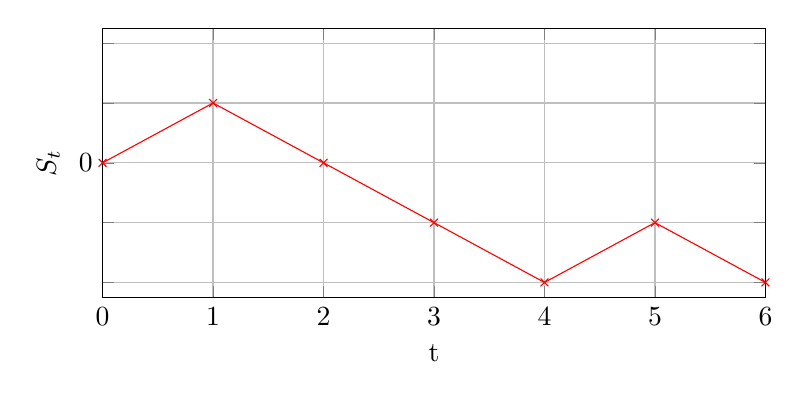
\begin{tikzpicture}
         \begin{axis}
        [width=10cm, height=5cm, xmin=0, xmax=6, ymin=-2.25, ymax=2.25, xmajorgrids=true, ymajorgrids=true, xtick={0,1,2,3,4,5,6}, ytick={-2,-1,0,1,2}, yticklabels={,,0,,},xlabel = t,ylabel = $S_t$]
        \addplot[color=red,mark=x] coordinates {(0,0) (1,1) (2,0) (3,-1) (4,-2) (5,-1) (6,-2)};
        \end{axis}
    \end{tikzpicture}
    \caption{Ejemplo de \textit{Paseo Aleatorio}.}
    \end{figure}
\end{itemize}
 Para valores de $t$ suficientemente grande, y escalando tiempo y espacio adecuadamente, el gráfico de $S_t$ toma la siguiente forma.\\ \newpage
\begin{figure}[h]
    \centering
    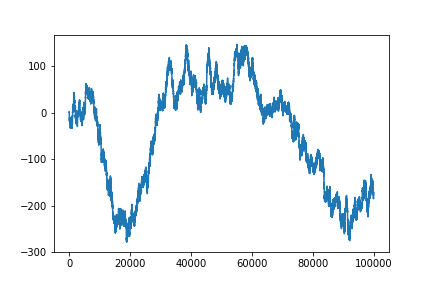
\includegraphics[width=0.6\textwidth]{browniano.png}
\end{figure}

Específicamente, el escalamiento corresponde al siguiente: $\forall\, a>0$, definimos
\[B_t^{(a)}:= \frac{1}{a}S_{ta^2}\]
\newline Estudiaremos la distribución de $B_t^{(a)}$: para $a>0$ fijo y $n\in \N$ (ambos suficientemente grandes), tomar $t=\frac{n}{a^2}$. Luego
\[B_t^{(a)} = \sqrt{\frac{t}{n}}S_n = \sqrt{t}\,\, \frac{1}{\sqrt{n}}\sum_{i=1}^n X_i\]
Ocupando $T.C.L.$, y recordando que $\E(X_i)=0$ y $Var(X_i)=1$, notamos que:
\[\frac{1}{\sqrt{n}}\sum_{i=1}^n X_i \approx Z\,\sim\,\mathcal{N}(0,1), \]
por lo tanto, concluímos que:
\[B_t^{(a)} \approx \sqrt{t}\,\,\mathcal{N}(0,1) = \mathcal{N}(0,t).\]
También es directo ver que, para valores enteros $m>n$, la variable $S_m-S_n$ es independiente de $S_n$ (puesto que la colección $(X_i)_i$ era $i.i.d$), es decir; $(S_n)_{n\in\N}$ posee la propiedad de \textbf{Incrementos Independientes}, lo cual se manifiesta también en $(B_t^{(a)})_{t\geq 0}$. (ver \cite[cap. 2]{Kara})\\ \newline
Lo anterior motiva la siguiente definición.

\begin{definicion}[Movimiento Browniano] Un Movimiento Browniano es un proceso estocástico\footnote{Es decir, una colección de variables aleatorias definidas en algún espacio de probabilidad $(\Omega,\mathcal{F},\prob)$, indexada por la variable $t\geq 0$.}, denotado $(B_t)_{t\geq 0}$, que satisface:
\begin{enumerate}
    \item[i.] $B_0 = 0$, $c.s.$
    \item[ii.] Posee incrementos independientes: $\forall\, t\geq 0$, $(B_{t+s}-B_t)_{s\geq 0}$ es independiente de $(B_s)_{0\leq s\leq t}$.
    \item[iii.] Posee incrementos normales: $\forall\, t,s\geq 0$, $B_{t+s}-B_{t}\,\sim\,\mathcal{N}(0,s)$.
    \item[iv.] Es un proceso contínuo; con probabilidad 1, la función $t\rightarrow\,B_t$ es contínua en $t$.
\end{enumerate}
\end{definicion}

La ley del proceso $(B_t^{(a)})_{t\leq 0}$ converge, cuando $a\rightarrow\,\infty$, a la ley del movimiento browniano $(B_t)_{t\geq 0}$, en un sentido adecuado (Teorema de Donsker, ver \cite[cap.2, Teo.4.2]{Kara}).\\ \newline $(B_t)_{t\geq 0}$ también es llamado \textbf{Proceso de Weiner}. El nombre "browniano" fue puesto en honor al botánico escocés, Robert Brown, quién observó el movimiento errático de partículas de polen en el agua en 1827. Porsteriormente, en 1905, el físico Albert Einstein explicaría este movimiento como resultado  de muchas pequeñas colisiones de polen con las moléculas de agua circundantes.\\ \newline
Pero, ¿realmente existe un proceso tal que cumpla $i$, $ii$, $iii$, y $iv$, de la difinición anterior?
\begin{teorema}
El Movimiento Browniano existe.
\end{teorema}
\textbf{Demostración: }ver \cite[cap. 2]{Kara}.\\ \newline

\begin{prop}Sea $(B_t)_{t\geq 0}$ Movimiento Browniano ($M.B.$), $\forall\, 0=t_0<t_1<t_2<\cdots<t_n$, la colección
\[\left(\frac{B_{t_i}-B_{t_{i-1}}}{\sqrt{t_i-t_{i-1}}}\right)_{i=1,\cdots,n}\]
son $i.i.d.$ $\mathcal{N}(0,1)$.
\end{prop}
\textbf{Demostración: }Directo de la definición de $M.B$.\\\rule{0.7em}{0.7em}\\ \newline
Esto da lugar  a un método sencillo para generar un $M.B.$ discretizado: para un horizonte $T>0$, y $n\in\N$, sea $\Delta t = T/n$, y $t_i = i\Delta t$. Dado $Z_1,\cdots, Z_n$,  $i.i.d.$ $\mathcal{N}(0,1)$, entonces el proceso $(Y_t)_{t\in [0,T]}$, definido como 
\[Y_{t_i}:= \sqrt{\Delta t}\,\sum_{j=1}^i Z_i\]
interpolando linealmente entre los $t_i$'s para los valores en $[0,T]\backslash\{t_0,\cdots,t_n\}$, es una aproximación de $(B_t)_{t\in[0,T]}$ (de hecho, tiene la misma ley en la malla $0=t_0<t_1<\cdots<t_n=T$).

\begin{prop} Sea $(B_t)_{t\geq 0}$ un $M.B.$:
\begin{enumerate}
    \item[a.] $\forall\,t_0>0$, el proceso $X_t := B_{t+t_0}-B_{t_0}$ es un $M.B.$. (Invarianza bajo shift)
    \item[b.] $\forall\,c>0$, el proceso $X_t := \frac{1}{\sqrt{c}}\,B_{ct}$ es un $M.B.$ (Invarianza bajo escalamiento)
    \item[c.] El proceso $X_t := B_1 - B_{1-t}$ es un $M.B.$ en $[0,1]$. (Propiedad de tiempo reverso)
    \item[d.]  El proceso $X_t:=tB_{1/t}$ es un $M.B.$ (con $X_0 =0$). (Inversión del tiempo)
    \item[e.] el proceso $X_t:=-B_t$ es un $M.B.$ (Simetría)
\end{enumerate}
\end{prop}
\textbf{Demostración: }ver \cite[cap. 2]{Kara}.\\ \newline
A pesar de ser contínuas, las trayectorias de un movimiento browniano son bastante irregulares. La \textit{trayectoria} de un $M.B.$ es la función (aleatoria)
\[t\rightarrow\,B_t\]
\begin{teorema}
\[\prob\left(\exits\,t\geq 0\,:\,B_t\,\text{es derivable en }t\right) = 0\]
\end{teorema}

\newpage
\begin{thebibliography}{X}
\bibitem{Bill} \textsc{Billingsley, P.},
\textit{Convergence of Probabilistic Measure}, second edition,
Wiley series in probability and statistic, 1999.

\bibitem{water} \textsc{University of Waterloo} ,
Notas de curso "STAT 901: Probability" formato PDF,
\texttt{http://sas.uwaterloo.ca/$\sim$dlmcleis/s901/s901\_2005.pdf}, 2005.

\bibitem{Pard} \textsc{Pardoux, E.}, \textit{Markov Processes and Applications},
Wiley series in probability and statistic, 2008.

\bibitem{Kara} \textsc{Karatzas, I.};\textsc{ Shreve, S.}, \textit{Brownian Motion and Stochastic Calculus}, Second Edition, Editorial Springer, 1991.

\bibitem{Lam} \textsc{Lampeyre, B.; Lamberton, D.} \textit{Introduction to Stochastic Calculus Applied to Finance}, Second Edition, CHAPMAN&HALL/CRC, 2008.
\end{thebibliography}

\end{document}
 